 %###############################################################################
% Template fuer eine Abschlussarbeit mit LaTeX

\NeedsTeXFormat{LaTeX2e}
\documentclass[a4paper]{book}

% LaTeX-Zusatzpakete
%\usepackage{german}                % deutsches Dokument (Trennung etc.)
\usepackage[ngerman]{babel}
\usepackage[utf8]{inputenc}
\usepackage{times}                 % Times Font
\usepackage{graphicx}              
\usepackage{multirow}
\usepackage{tabularx}              % erweiterte Tabellenmöglichkeiten
\usepackage{subfig}                % Teilgrafiken erlauben
\usepackage{amsfonts}              % fuer zusätzliche math. Symbole
\usepackage{amssymb}               % weitere math. Symbole
\usepackage{theorem}               % Theorem-Umgebung
\usepackage{listings}              % Programmlistings
\usepackage[table,xcdraw]{xcolor}
\usepackage{setspace}
\usepackage{wrapfig}
\usepackage{verbatim}
\usepackage{xurl}
\usepackage[T1]{fontenc}
\usepackage{tikz}
\usetikzlibrary{automata, positioning, arrows, shapes.geometric}


\usepackage{titlesec}
\titleformat*{\subsubsection}{\large\bfseries}

\tikzset{
->, % makes the edges directed
>=stealth', % makes the arrow heads bold
node distance=5cm, 
auto,
%every state/.style={thick, fill=gray!10}, % sets the properties for each ’state’ node
elliptic state/.style={draw,ellipse},
initial text=$ $, % sets the text that appears on the start arrow
}



% Steuerung fuer Programmlistings (anpassen an Programmiersprache)
% \lstset{language=Python, frame=single, breaklines=true, tabsize=2}
%\lstset{basicstyle=\ttfamily,
%  showstringspaces=false,
%  commentstyle=\color{red},
%  keywordstyle=\color{blue}
%}


\lstset{frame=tb,
  aboveskip=3mm,
  belowskip=3mm,
  showstringspaces=false,
  columns=flexible,
  basicstyle={\small\ttfamily},
  numbers=none,
  numberstyle=\tiny\color{gray},
  keywordstyle=\color{blue},
  commentstyle=\color{gray},
  stringstyle=\color{violet},
  breaklines=true,
  breakatwhitespace=true,
  tabsize=3,
  captionpos=b
}


%###############################################################################
% Grössenangaben zum Dokument etc.

% vertikal
\setlength{\voffset}{-0.5cm}
\setlength{\textheight}{23cm}
\setlength{\topmargin}{0cm}
\setlength{\headheight}{6mm}
\setlength{\headsep}{1cm}
\setlength{\topskip}{0cm}
\setlength{\footskip}{1cm}

% horizontal
\setlength{\hoffset}{-0.4cm}
\setlength{\textwidth}{15.5cm}
\setlength{\oddsidemargin}{0.8cm}
\setlength{\evensidemargin}{0.8cm}

\setlength{\parindent}{1.5cm}        % kein Einzug bei Paragrafenbeginn


%###############################################################################
% Hier geht es los

% Autor und Abgabedatum ändern
\def\autor{Henry Weckermann}
\def\datum{\today{}}

% Titelseite erzeugen
\begin{document}


%###############################################################################
% Titelseite

\sloppy
\pagestyle{headings}
\bibliographystyle{ieeetr}
\pagenumbering{roman}


% Basierend auf der Fachschaftsvorlage
\begin{titlepage}
  \textbf{
    \begin{tabular}[t]{>{\vspace*{0pt}}p{0.45\textwidth}c>{\vspace*{0pt}}p{0.45\textwidth}}
      {
        \begin{tabular}{ll}
          \begin{tabular}{l}
            \raisebox{1.5\height}{
\includegraphics[width=0.13\textwidth]{images/fhlogo}} 
          \end{tabular}
          &
          \begin{tabular}{l}
            {\small{\sffamily Hochschule}}\\
            {\small{\sffamily Bonn-Rhein-Sieg}}\\
            {\footnotesize{\itshape University of Applied Sciences}}\\
            \\
              {\small{\sffamily Fachbereich Informatik}}\\
              {\footnotesize{\itshape Computer Science Department}}\\
          \end{tabular}
        \end{tabular}
      }
      &
      \hspace*{0.1\textwidth}
      &
      \begin{tabular}{r}
% hier evtl. Firma nennen mit/ohne Logo, ansonsten auskommentieren
        \hfill 
\includegraphics[width=0.3\textwidth]{images/firmenlogo}\\
      \end{tabular}
    \end{tabular}
  } %\textbf
  
  
  \renewcommand{\baselinestretch}{1.4}\normalsize
  
  \vspace{3cm}
  \begin{center}
    
% einen Typ auswählen
    \begin{Huge}\textbf{Abschlussarbeit}\end{Huge}\\
    \vspace{0.8cm}
% einen Studiengang auswählen
    \begin{Large}\textbf{im Bachelorstudiengang Informatik}\end{Large}\\
    
    \vspace{2.2cm}
    \renewcommand{\baselinestretch}{1}\normalsize
    \begin{huge}
    \color{blue}
      \textbf{Untersuchung der Sicherheit von OpenWrt 
anhand der BSI TR-03148 mittels eines OpenWrt 
betriebenen Heim-Routers \\}
    \end{huge}
    \renewcommand{\baselinestretch}{1.5}\normalsize
    \vspace{0.7cm}
    
    
    \begin{Large}\textbf{von \autor\ \\}
    \end{Large}
  \end{center}
  
  \vspace{4.5cm}
  
  \begin{large}
    \textbf{
      \begin{tabular}{ll}
      Erstbetreuer:  & Prof. Markus Ullmann\\
      Zweitbetreuer: & Prof. Dr. Norbert Jung\\
      Betreuer im BSI: & Florian Bierhoff\\
      				  & \\	
      Eingereicht am: & 25.01.2021 \\
      \end{tabular}
    }
  \end{large}
\end{titlepage}


%###############################################################################
% Erklärung
\begin{large}

\section*{Erklärung}

Hiermit erkläre ich an Eides Statt, dass ich die vorliegende Arbeit
selbstständig und ohne Benutzung anderer als der angegebenen
Hilfsmittel angefertigt habe. Die aus fremden Quellen direkt oder
indirekt übernommenen Gedanken sind als solche kenntlich gemacht.  Die
Arbeit wurde bisher in gleicher oder ähnlicher Form noch keiner
anderen Prüfungsbehörde vorgelegt bzw. nicht veröffentlicht.\\

\vspace{1cm}
\noindent
Bonn, den 25.01.2021
\vspace{2cm}

\noindent
\rule{10cm}{0.1mm} \\
\autor\


%###############################################################################
% Abstract

\clearpage
\section*{Abstract}
\begin{onehalfspace} 
In an increasingly digitalized world, the network router often forms the border between the home network and the internet. An increasing number of attacks on these very home networks for the spread of ransomware and botnets is observed worldwide \cite[p.~11-15]{BundesamtfurSicherheitinderInformationstechnik.2020}. This makes it more important for manufacturers and customers to evaluate the security of their products. The goal of this thesis was to evaluate the open-source router operating system OpenWrt using the “Technical Guideline 03148 - Secure Broadband Routers“ of the German Federal Office for Information Security. Furthermore, solutions for shortcomings of OpenWrt were worked out in cases were OpenWrt could not comply with the guideline. To address another possibility for security verification the source code of various open source router operating systems were statically analyzed. Finally, the results of this analysis were compared with the results of the “Home Router Security Report 2020“. \\
\indent To support the premise that OpenWrt is compliant with the Technical Guideline, all applicable test cases were tested against the published test criteria. Furthermore, the source codes of seven contemporary open source router firmware images were statically analyzed using the “Firmware Analysis and Comparison Tool“ so that the results were comparable to the “Home Router Security Report 2020“. The results showed that OpenWrt fails to comply in 22\% of the test cases, but the predicted effort to correct these weaknesses is low. The static code analysis showed that the open source firmware, while not without shortcomings, is superior to the proprietary firmware which was analyzed in the “Home Router Security Report“. \\
\indent The results showed that, with some adjustments, OpenWrt can present a safer alternative to proprietary pre-installed router firmware and that open source firmware performs comparatively well when using static code analysis. Ultimately, a repetition of the static code analysis with a larger set of open-source firmware is desirable in order to establish a higher degree of comparability. 
\end{onehalfspace} 


\clearpage
\section*{Zusammenfassung}
\begin{onehalfspace}  

In einer zunehmend digitalisierten Welt bildet der Netzwerk-Router häufig die Grenze zwischen dem Heimnetzwerk und dem Internet. Weltweit wird eine zunehmende Anzahl an Angriffen auf eben diese Heimnetze für die Verbreitung von Ransomware und Bot-Netzen beobachtet \cite[p.~11-15]{BundesamtfurSicherheitinderInformationstechnik.2020}. Umso wichtiger sind Mittel und Wege für Hersteller und Kunden die Sicherheit ihrer Produkte zu evaluieren. Das Ziel dieser Arbeit war es das quelloffene Router-Betriebssystem OpenWrt mittels der "`Technischen Richtlinie 03148 - Sichere Breitband Router"' des deutschen Bundesamtes für Sicherheit in der Informationstechnik (BSI) zu prüfen. Ferner sollten Lösungen für eventuelle Defizite erarbeitet werden, falls OpenWrt den Anforderungen der TR nicht entsprechen kann. Anschließend wurde der Quellcode verschiedener quelloffener Router-Betriebssysteme statisch analysiert, um eine weitere Möglichkeit der Sicherheitsüberprüfung zu thematisieren. Die Ergebnisse dieser Analyse wurden abschließend mit den Ergebnissen des "`Home Router Security Reports 2020“ verglichen. \\
\indent Um die Annahme zu stützen, dass OpenWrt TR-konform ist, wurden alle anwendbaren Testfälle anhand der veröffentlichten Prüfkriterien getestet. Weiterhin wurde der Quellcode von sieben quelloffenen Router Firmware-Abbildern statisch mit dem "`Firmware Analysis and Comparison Tool“ analysiert, sodass die Ergebnisse mit dem "`Home Router \mbox Security Report 2020“ vergleichbar waren. Die Ergebnisse zeigten, dass OpenWrt 22\% der Technischen Richtlinie nicht besteht, der Aufwand aber gering ist, diese Defizite auszubessern. Die statische Code-Analyse zeigte, dass die quelloffene Firmware zwar nicht ohne Mängel ist, jedoch im Vergleich der proprietären Firmware überlegen ist. \\
\indent Die Ergebnisse zeigen, dass OpenWrt mit einigen Anpassungen eine sichere Alternative zu proprietärer vorinstallierter Firmware bilden kann und die quelloffene Firmware bei einer statischen Code-Analyse vergleichsweise gut abschneidet. Letztlich ist eine Wiederholung der statischen Code-Analyse mit einem größeren Korpus erstrebenswert, um eine höhere Vergleichbarkeit herzustellen. 

\end{onehalfspace}
  
  
\clearpage

\section*{Abkürzungsverzeichnis}
\let\cleardoublepage\clearpage
\begin{table}[!ht]
\centering
\begin{tabular}{ll}
BSI   & Bundesamt für Sicherheit in der   Informationstechnik                             \\
CA      & Certificate Authority                \\
CCC     & Chaos Computer Club                  \\
CNA     & CVE Numbering Authorities            \\
CPE     & Common Platform Enumeration          \\
CSRF    & Cross-Site-Request-Forgery           \\
CSS     & Cascading Style Sheets               \\
CVE     & Common Vulnerabilities and Exposures \\
CVSS    & Common Vulnerability Scoring System  \\
(D)DoS    & (Distributed) Denial of Service        \\
DHCP    & Dynamic Host Configuration Protocol  \\
DNS     & Domain Name System                   \\
DUT     & Device under Test.                   \\
EOL     & End Of Life                          \\
FACT  & Firmware Analysis   and   Comparison Tool                                         \\
FIRST & Forum of Incident Response and Security Teams                                     \\
FKIE  & Fraunhofer-Institut für   Kommunikation,   Informationsverarbeitung und Ergonomie \\
GOT     & Global Offset Table                  \\
GPL     & GNU General Public License           \\
ICS     & Implementation Conformance Statement \\
IDE     & Integrated Development Environment   \\
IoT     & Internet of Things                   \\
IP      & Internet Protocol                    \\
ISP     & Internet Service Provider            \\
LAN     & Local Area Network                   \\
LuCI    & OpenWrt web user interface           \\
NAT     & Network Address Translation          \\
NTP     & Network Time Protokoll               \\
NX-Bit  & No eXecute Bit                       \\
OpenWrt & Open Wireless Router                 \\
OWASP	& Open Web Application Security Project \\
PIE     & Position-Independent Executables     \\
RATS    & Rough Auditing Tool for Security     \\
RELRO   & RELocation Read-Only                 \\
SCP     & Secure Copy                          \\
SDK     & Software Developer Kit               \\
SE      & Secure Element                       \\
SIP     & Session Initiation Protocol          \\
SMTP    & Simple Mail Transfer Protocol        \\
SOHO    & Small Office, Home Office            \\
TEE     & Trusted Execution   Environment      \\
TFTP    & Trivial File Transfer Protocol       \\
VoIP    & Voice over IP                        \\
VPN     & Virtual Private Network              \\
VPS     & Virtual Private Server               \\
WAN     & Wide Area Network                    \\
WPA     & Wi-Fi Protected Access               \\
WPS     & Wi-Fi Protected Setup 
\end{tabular}
\end{table}

\let\cleardoublepage\cleardoublepage


%###############################################################################
% Inhaltsverzeichnis

\tableofcontents           % Inhaltsverzeichnis generieren
\cleardoublepage
\pagenumbering{arabic}


%###############################################################################
% Kapitel 1

\chapter{Einleitung}

\section{Ausgangspunkt}

\begin{onehalfspace}
Das Internet wird ein zunehmend wichtigerer Teil des menschlichen Lebens. Öffentliche Hotspots, internetfähige Alltags-Geräte (Internet of Things (IoT) Geräte) und mobiles \mbox Arbeiten von Zuhause sind nur einige Beispiele für technologische Neuerungen, welche \mbox ohne das Internet nicht möglich wären. Die rund 38 Mio. Netzanbindungen an DSL-, Kabel-, oder Glasfaser-Anschlüsse in Deutschland werden in Heimnetzen und Kleinunternehmen überwiegend durch Netzwerk-Router realisiert \cite{StatistischesBundesamt.2020}. In vielen Fällen bildet der Router die direkte Schnittstelle zwischen dem Internet und dem privaten Netzwerk. So stellt dieser durch Paketfilter und eine Firewall meist auch die einzige zentrale Sicherheitskomponente zum Schutz des Netzwerkes bereit. Ein erfolgreicher Angriff auf den Router bietet einem Angreifer unzählige Möglichkeiten, in das Netz einzugreifen und so immensen Schaden anzurichten. Neben bekannten Zielen wie private Daten und Passwörtern kann der Router auch als Teil eines Bot-Netzwerks für\mbox{} Distributed Denial-of-Service (DDoS) verwendet werden oder als Einfallstor auf \mbox weitere Geräte des Netzwerkes \cite{Triantopoulou.15.07.201917.07.2019}. In Korrelation mit den stark steigenden Fällen von Cyber\-kriminalität im privaten und wirtschaftlichen Umfeld zeigt dies wie wichtig ein von Werk aus geschützter Router mit einer sicheren Konfiguration ist  \cite{BundesamtfurSicherheitinderInformationstechnik.2020}.
\newline\indent Handelsübliche Router, wie sie in Privathaushalten und Small Office, Home Office (SOHO) Umgebungen eingesetzt werden sind bereits mit einem proprietären Betriebssystem bespielt. Die Sicherheit dieser meist proprietären Distribution kann nur mit großem Aufwand von Endnutzern verifiziert werden und Sicherheitsupdates nur vom Hersteller veröffentlicht werden. Hersteller können in der zunehmend kürzer werdenden Zeit zwischen neuen Iterationen von Malware meist nicht in angemessener Zeit reagieren, um Sicherheitsupdates zur Verfügung zu stellen. Quelloffene Router Firmware wie OpenWrt, DD-Wrt, Tomato oder \mbox LibreCMC bieten eine Alternative zu den vorinstallierten, proprietären Betriebssystemen der Router \cite{OpenWrtWebseite.,DDWRTWebseite.,AdvancedTomatoWebseite.,libreCMCWebseite.}. Diese Projekte können vollständig eingesehen, modifiziert und kompiliert werden, sodass die Sicherheit des Produktes einfacher evaluiert werden kann. Ebenfalls können aufgrund der hohen Anzahl an Mitwirkenden Sicherheits- und Funktionsupdates \mbox schneller entwickelt und veröffentlicht werden. Umfangreiche Überprüfungen dieser Projekte, wie z.B. anhand der BSI TR-03148: Sichere Broadband Router, werden allerdings aufgrund des hohen Zeit- bzw. Kostenaufwands selten durchgeführt, sodass diese Zertifizierung nicht erlangen können \cite{BundesamtfurSicherheitinderInformationstechnik.2020b}. Eine solche Zertifizierung könnte ungeschulten Endnutzern auch diese quelloffenen Router-Betriebssysteme als Alternativen näherbringen und somit zu einem höheren Sicherheitsniveau in privater und SOHO Netzwerkinfrastruktur führen.

\end{onehalfspace}


\section{Verwandte Arbeiten}
\begin{onehalfspace}
Während der Einsatz von OpenWrt im privaten und professionellen Umfeld beliebt zu sein scheint (vgl. Abschnitt \ref{OpenWrt Relevanz}) und auch einige Forschungsarbeiten mit OpenWrt verwirklicht wurden, sind derzeit keine aktuellen Arbeiten zur Sicherheit von OpenWrt verfügbar. Ortega et al. (2009) veröffentlichte eine Arbeit über eine quelloffene Methode zum Verhindern von sogenannten ARP Poisoning Attacken. Sie nutzten in diesem Kontext OpenWrt lediglich als vielseitig unterstützte Testplattform \cite{Ortega.19.10.200921.10.2009}. Palazzi et al. (2010) nutzten den Funktionsumfang und die Anpassbarkeit der Firmware, um einen verbesserten Datendurchsatz in Heimnetzen mit verschiedenen WLAN-Geräten zu erreichen \cite{Palazzi.19.07.201023.07.2010}. Keine der derzeitigen Veröffentlichungen beschäftigt sich mit der Sicherheit von OpenWrt als Betriebssystem. Einzig Andrew McDonnell (2014) veröffentlichte in seinem Blog zwei Einträge über eine Sicherheitsanalyse von OpenWrt mittels des Tools checksec.sh (\begin{small}\url{https://github.com/slimm609/checksec.sh}\end{small}) und entwarf eine verbesserte Version, in welcher bedeutend mehr Maßnahmen zur Verhinderung von Exploits aktiviert waren \cite{AndrewMcDonnell.2014}. Die Ergebnisse der Veröffentlichung basierten jedoch auf Version 14.07 (Barrier Breaker) von OpenWrt, welche stark veraltet ist \cite{OpenWrtWebseite.13.12.2020}.	\newline \indent
 	Die Forschung an Komponenten, die OpenWrt ausmachen, ist jedoch keinesfalls so eingeschränkt wie zuvor aufgezeigt. Der Linux Kernel, welcher einen grundlegenden Teil des OpenWrt Betriebssystems ausmacht, ist seit seiner Veröffentlichung 1991 ein andauerndes Gebiet der Forschung und Entwicklung, so auch in der IT-Sicherheit \cite{LinusTorvalds.1991, JonathanCorbet.2016, Chen.2011b, Jimenez.06.12.201609.12.2016}. Ebenso definiert sich OpenWrt über seine ca. 3800 zusätzlichen quelloffenen Pakete. \mbox Viele dieser Software-Erweiterungen existieren schon seit Jahrzehnten und ihre Integrität und Vertraulichkeit sind von den unzähligen Nutzern auf verschiedensten Plattformen anerkannt \cite{LennartBeringerAdamPetcheKatherineQ.YeAndrewW.Appel., Viega.2009, Barayuga.24.08.201527.08.2015}. Abschließend kann man festhalten, dass es zwar durchaus Forschung an Komponenten, welche auch in OpenWrt genutzt werden, gibt, jedoch OpenWrt selbst noch nicht im Mittelpunkt der Forschung stand und die Sicherheitslage des Projektes weitestgehend ungeklärt bleibt.

\end{onehalfspace}


\section{Zielsetzung}	
\begin{onehalfspace}
Ziel dieser Arbeit war es, die Technische Richtlinie 03148 des BSI an Version 19.7.04 von OpenWrt durchzuführen und das Router-Betriebssystem auf Konformität zu prüfen. Hierbei wurde ein TP-Link Archer C7 Router genutzt. Es wurden die grundsätzlichen Sicherheitsmerkmale von OpenWrt mittels der Technischen Richtlinie evaluiert (siehe Abschnitt \ref{Testfälle}). Dabei wurde nur die Funktionalität des Betriebssystems geprüft, welche nach der \mbox Installation auf dem Gerät bereitgestellt wurde. Funktionen, welche vom Nutzer zusätzlich installiert und eingerichtet werden mussten, wurden nicht betrachtet. Wenn es der Testfall angeboten hat wurde ein automatischer Test entwickelt, sodass eine wiederholte Durchführung beschleunigt werden kann. Ebenso wurde die Anwendbarkeit der Technischen Richtlinie auf quelloffene Netzwerk-Betriebssysteme ermessen. Darüber hinaus wurden statische Softwaretests einiger quelloffener Router-Betriebssysteme mittels des \glqq Firmware Analysis and \mbox Comparison Tools\grqq{} als weitere Metrik genutzt, um einen differenzierteren Einblick in die Sicherheitslage solcher Projekte zu gewähren (siehe Abschnitt \ref{statische CodeA}). Die Ergebnisse dieser Analyse wurden darauffolgend mit den Ergebnissen des \glqq Home Router Security Report 2020\grqq{} des Fraunhofer-Instituts für Kommunikation, Informationsverarbeitung und Ergonomie (FKIE) verglichen (siehe Abschnitt \ref{erg_statisch}). Abschließend wurde sich kritisch mit den Ergebnissen, sowie der technischen Richtlinie, auseinandergesetzt (vgl. Abschnitt \ref{discussion}).  Die in dieser wissenschaftlichen Untersuchung genutzte Vorgehensweise kann nicht die vollständige Sicherheit aller Aspekte der Software OpenWrt nachzuweisen. Es muss immer betont werden, dass viele potenziell wichtige Aspekte einer sicheren Software nicht in Betracht gezogen \mbox werden. Vielmehr soll eine Grundlage bzw. ein möglicher Einstiegspunkt für weitere Forschung an Methoden und Abläufen zum Testen von Open Source (Router-) Software geschaffen \mbox werden. Die Ergebnisse der Arbeit können sowohl der Entwicklung von OpenWrt als auch Endnutzern weitere Einblicke in die Sicherheit des Projektes liefern und somit langfristig die Resilienz der Heimnetz-Infrastruktur stärken. 

\end{onehalfspace}


%###############################################################################

\chapter{Grundlagen}


\section{Netzwerkrouter}
\label{Router}
\begin{onehalfspace}

Ein Netzwerkrouter (auch als Router bezeichnet) ist ein essentieller Bestandteil der meisten Computer-Netzwerke und kann auf Schicht 3 des OSI-Referenzmodelles (vgl. Abbildung \ref{fig:OSI}) Netzwerkpakete zwischen mehreren Netzwerken weiterleiten \cite[p.~48]{Lowe.2018}. Eine häufige Verwendung von Routern ist die Anbindung eines privaten Netzwerkes an das Internet. Da Router auf Schicht 3 des OSI-Modells arbeiten, nutzen sie das IP-Protokoll um Netzwerkpakete weiterzuleiten \cite[p.~48]{Lowe.2018}. Eine wichtige Aufgabe des Routers ist unter anderem die sog. \glqq Network Address Translation (NAT)\grqq . Diese Technik wird eingesetzt, um den Netzwerkverkehr aller Systeme im privaten Netzwerk durch den Router in das öffentliche Netz (Internet) zu transportieren und dort an die korrekte IP-Adresse zuzustellen \cite{Perlman.1999}. Im Gegensatz zu Netzwerk-Bridges (auch \glqq Netzwerk-Switches\grqq{} genannt) sind Router flexibler, da sie mit logischen Adressen (IP-Adressen) arbeiten \cite[p.~714]{Fischer.2011}. Bridges hingegen arbeiten auf der Sicherungsebene (Schicht 2) des OSI-Modells. Dadurch können sie nicht verwendet werden, um ein anderes Sub-Netz zu adressieren. Daraus folgt ebenso, dass Netzwerk-Bridges nicht für die Verbindung eines privaten Netzwerks mit dem Internet geeignet sind \cite[p.~48]{Lowe.2018}. \\
\indent Neben den bereits genannten Aufgaben eines Routers liefern die meisten modernen Heimrouter zusätzliche Funktionen. So verfügen moderne Heimrouter meist auch über die Möglichkeiten einer Firewall. Durch diese können ein- und ausgehende Pakete gefiltert werden, oder Angriffe auf das Netzwerk erkannt werden \cite[p.~588]{Schemberg.2016}. Ebenfalls bieten viele Router einen \glqq Dynamic Host Configuration Protocol (DHCP)\grqq -Server an. Dieses Protokoll ermöglicht die automatische Zuweisung einer Netzwerkkonfiguration an Clients \cite[p.~222]{Fischer.2011}. Darüber hinaus findet man häufig auch einen \glqq Network Time Protocol (NTP)\grqq -Server, welcher genutzt werden kann, um über den Router Zeitinformationen zu beziehen \cite[p.~577]{Fischer.2011}. Zusätzlich verfügen einige Heimrouter über die Möglichkeit das \glqq Voice over IP (VoIP)\grqq{} Protokoll zu nutzen, welches Telefonie über das Internet ermöglicht \cite[p.~911]{Fischer.2011}. Einige Modelle unterstützen auch \glqq Virtual Private Networks\grqq{}(VPN) . Dabei handelt es sich um \mbox eine sichere Verbindung von zwei privaten Netzwerken über ein öffentliches Netzwerk, \mbox also dem Internet. Die Daten sind auf dem Weg vollständig verschlüsselt, sodass abgefangene Pakete keinen Aufschluss über den Inhalt geben. In diesem Zusammenhang wird auch von einem \glqq Tunnel\grqq gesprochen, da die einzigen Zugangspunkte an den jeweiligen Enden sind \cite[p.~50]{Lowe.2018}.

\begin{figure}[ht]
\begin{center}
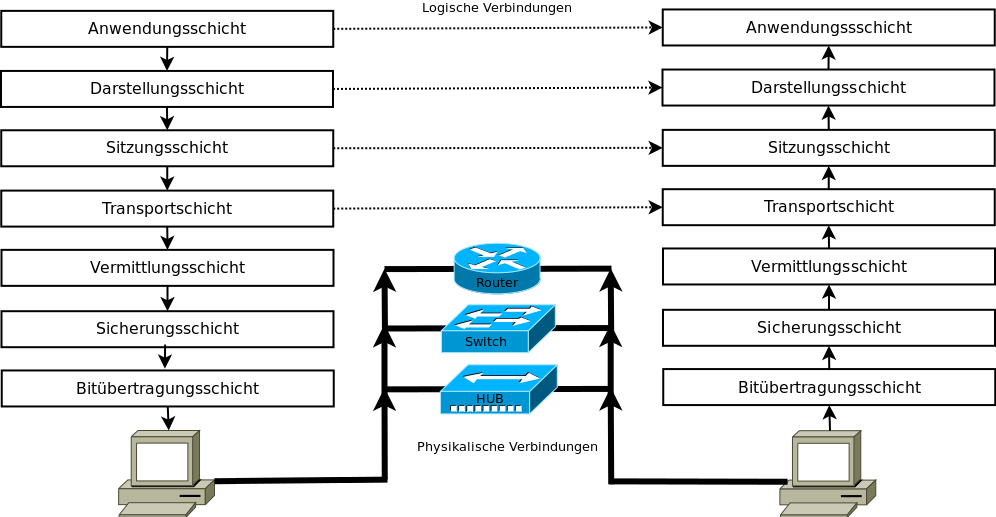
\includegraphics[scale=0.35]{images/OSI} 
\caption{Abbildung des OSI-Referenzmodells \cite{Wiki.2011}.}
\label{fig:OSI}
\end{center}
\end{figure}	

\end{onehalfspace}


\section{Angriffe auf Netzwerkroutern}
\label{Angriffe}

\begin{onehalfspace}

Router sind ein immer beliebteres Angriffsziel für Cyberkriminelle \cite{StephenHilt.2020}. Der Netzwerkrouter stellt oft die direkte Schnittstelle zwischen dem Internet und einem privaten Netzwerk dar. Die Übernahme von Routern bietet Angreifern daher viele Monetarisierungsmöglichkeiten. Router bieten ein geeignetes Einfallstor in ein privates Netz, da Angreifer über einen kompromittierten Router Zugriff auf weitere Geräte des privaten Netzes erhalten können. Der Router und die ggf. weiteren infizierten Geräte können nun z.B. für die Verbreitung von Ransomware eingesetzt werden, oder selbst Opfer eines Ransomware-Angriffs sein. Bei diesem Angriff wird der Zugriff auf die Daten des Geräts von einem Angreifer verhindert, bis das Opfer den geforderten Betrag bezahlt. Ein kompromittierter Router kann auch als Teil eines Bot-Netzes eingebunden und für die Zwecke des Angreifers missbraucht werden. Darüber hinaus kann das Gerät auch genutzt werden, um den Datenverkehr des Angreifers über die IP-Adresse des Routers zu leiten, sodass die Spuren des Angreifers verwischt werden und die IP des infizierten Routers augenscheinlich illegale Aktivitäten durchführt \cite{StephenHilt.2020}.



\subsection{Bruteforce Angriffe}
\label{bruteforce}
Bei einem Bruteforce Angriff versucht ein Angreifer nicht eine bestimmte Software- oder Hardwarelücke auszunutzen, sondern stattdessen durch eine erschöpfende Suche des Schlüsselraumes das korrekte Passwort zu finden. Es können natürlich auch Kombinationen von Nutzername und Passwort gesucht werden, um sich auf einem Gerät anmelden zu können. Für diese Suche werden oft Passwortlisten oder Listen mit häufigen Kombinationen von Nutzername und Passwort eingesetzt. Es ist jedoch auch möglich automatisch einen voreingestellten Passwortraum, z.B. acht Zeichen mit einer Kombination aus Buchstaben und Zahlen, zu bilden und alle möglichen Kombinationen zu testen \cite{OWASP.2020}. Indem der Angreifer die Antwort des angegriffenen Servers oder Systems evaluiert, kann er einen Erfolg feststellen. Aus dem Vorgehen wird ersichtlich, dass dieser Angriffsvektor unter Umständen sehr zeitintensiv ist, wenn ein sicheres Passwort gewählt wurde (vgl. Tabelle \ref{tab:speed}). Wie Hilt et al. (2020) zeigten, gewinnen Bruteforce Angriffe auf Router jedoch stetig an Beliebtheit. Aufgrund von einfachen oder bekannten Standardpasswörtern ist es Angreifern möglich, schnell durch einen Bruteforce-Angriff Zugriff auf einen Router zu erhalten und diesen für eigene Zwecke zu nutzen \cite[p.~5]{StephenHilt.2020}. \\


\begin{table}[ht]
\centering
\resizebox{\textwidth}{!}{%
\begin{tabular}{llllllll}
\hline
\textbf{Zeichenraum} & \textbf{4 Zeichen} & \textbf{5 Zeichen} & \textbf{6 Zeichen} & \textbf{7 Zeichen} & \textbf{8 Zeichen} & \textbf{9 Zeichen} & \textbf{10 Zeichen} \\ \hline
26 {[}a-z{]}           & \textless{}1 Sekunde & \textless{}1 Sekunde & \textless{}1 Sekunde & 8 Sekunden & 4 Minuten  & 2 Stunden & 2 Tage     \\
52 {[}A-Z; a-z{]}      & \textless{}1 Sekunde & \textless{}1 Sekunde & 20 Sekunden          & 17 Minuten & 15 Stunden & 33 Tage   & 5 Jahre    \\
62 {[}A-Z; a-z; 0-9{]} & \textless{}1 Sekunde & \textless{}1 Sekunde & 58 Sekunden          & 1 Stunde   & 3 Tage     & 158 Tage  & 27 Jahre   \\
96 (mit Sonderzeichen) & \textless{}1 Sekunde & 8 Sekunden           & 13 Minuten           & 21 Stunden & 84 Tage    & 22 Jahre  & 2108 Jahre \\ \hline
\end{tabular}%
}
\caption{Benötigte Rechenzeit zum Finden eines Passwortes durch einen Bruteforce Angriff für verschiedene Zeichenräume und Zeichenanzahl bei der Berechnung von 1 Milliarden Schlüsseln pro Sekunde.}
\label{tab:speed}
\end{table}


\subsection{Cross-Site-Request-Forgery}
\label{CSRF}
Neben dem Bruteforce Angriff auf den Webserver ist auch Cross-Site-Request-Forgery (CSRF) ein Angriffsvektor, welcher bei Routern zum Einsatz kommen kann \cite{Stuttard.2011}. Wenn keine adäquaten Schutzmaßnahmen vom Server getroffen werden, kann ein Angreifer über eine präparierte Website oder einen \mbox Phishing Link schädlichen Code auf Webseiten ausführen, auf denen der Nutzer bereits authentifiziert ist. Dieser Code versetzt den Angreifer in die Lage, Befehle auf der Webseite oder dem Webserver auszuführen, auf welchem der Nutzer angemeldet ist \cite{Kim.2015}. Es könnte zum Beispiel ein neuer Benutzeraccount durch den Angreifer angelegt werden oder Einstellungen und Sicherheitsparameter an den Angreifer gesendet werden (siehe Abbildung \ref{fig:Cross-Site-Request-Forgery Ablauf}). So könnte ein Angreifer eine gültige Session eines Nutzers übernehmen, wenn dieser beim Webserver seines Routers angemeldet ist. Von dort könnte er Zugangsdaten entwenden und verändern oder einen persistenten Einstiegspunkt in das Netzwerk ermöglichen. Ebenso könnte ein präpariertes Firmware-Abbild aufgespielt werden. Es ist auch ein zweistufiges Verfahren bekannt, bei dem der Nutzer zunächst durch den Angreifer an seinem Gerät angemeldet wird, da das Opfer meist nicht an seinem Gerät angemeldet ist. Danach verläuft der CSRF-Angriff wie beschrieben. Dieses zweistufige Vorgehen ist möglich, da viele Endnutzer das Passwort ihres Gerätes nicht ändern und die voreingestellten Passwörter oft nach einem bekannten Muster generiert werden \cite{Stuttard.2011}.\\
\indent Eine häufig verwendete Sicherheitsmaßnahme gegen CSRF Angriffe ist ein Anti-CSRF Cookie (auch Token genannt). Dieser wird im \glqq HTTP-request-header\grqq , im \glqq http-POST-body\grqq{} oder als verstecktes Feld in einem \glqq HTTP-FORM-Objekt\grqq{} deklariert und besteht aus zwei zufällig generierten Zeichenketten, sodass der Nutzer und der Server jeweils einen Cookie gespeichert haben. Der Cookie des Nutzers wird für jede http-Methode benötigt, welche nach dem Setzen des Cookies aufgerufen wird. Dazu wird neben dem normalen Session Cookie auch geprüft, ob der korrekte Anti-CSRF Cookie übermittelt wurde. Dies geschieht auf Seiten des Servers mittels des zweiten Teils des CSRF-Tokens \cite{Yaworski.2019}. Wenn der Angreifer diesen Wert nicht berechnen kann, so kann er keine erfolgreiche domänenübergreifende Anfrage stellen. Um ein höheres Sicherheitsniveau zu erreichen sollte der CSRF-Cookie an die Session des Nutzers gebunden sein \cite{Stuttard.2011}. \\

\begin{figure}[ht]
\begin{center}
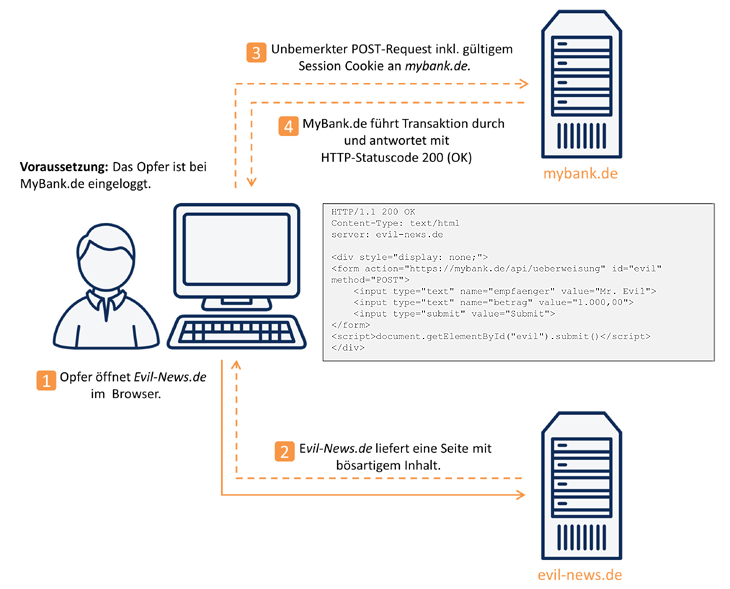
\includegraphics[scale=0.55]{images/CSRF} 
\caption{Ein möglicher Ablauf eines Cross-Site-Request-Forgery Angriffs. Der Nutzer ist bei MyBank.de angemeldet und öffnet Evil-News.de. Diese Seite liefert Schadcode an den Browser des Opfers aus. Der Code tätigt eine Überweisung mittels eines POST Requests und dem gültigen Cookie des Nutzers. Da es keine Abwehrmaßnahmen gibt tätigt der Bankserver die Überweisung an den Angreifer \cite{MartinMuller.2019}.}
\label{fig:Cross-Site-Request-Forgery Ablauf}
\end{center}
\end{figure}	


\subsection{DNS Rebinding Attacke}
\label{rebinding}
Bei dieser Art von Angriff wird die vom Browser durchgesetzte "`Same Origin Policy“ umgangen, um arbiträre Anfragen an das lokale Netzwerk des Opfers zu stellen. Abbildung \ref{fig:Same-Origin} zeigt, wie die Herkunft ("`Origin“) eines Web Dokumentes definiert ist.

\begin{figure}[ht]
\begin{center}
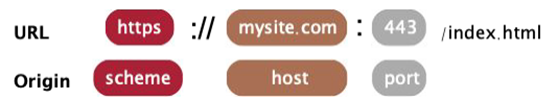
\includegraphics[scale=0.5]{images/Same_Origin_Policy} 
\caption{Origin (dt. Herkunft) eines Web-Dokumentes \cite{GeraldDoussot.2019}}
\label{fig:Same-Origin}
\end{center}
\end{figure}

\noindent Zwei Dokumente haben also die gleiche Herkunft ("`same origin“), wenn sie identische "`scheme“, "`host“ und "`port“ Komponenten haben. Die "`Same Origin Policy“ setzt durch, dass Skripte, oder auch Cascading Style Sheets (CSS), nur auf Daten von anderen Webseiten zugreifen können, wenn diese sich dieselbe Herkunft teilen. Wenn diese Richtlinie nicht implementiert wäre, dann wäre eine bösartige Webseite zum Beispiel in der Lage auf ein Bankkonto zuzugreifen, auf dem ein Opfer ebenfalls eingeloggt ist. Dort könnten Daten wie die Transaktionshistorie ausgelesen oder weitere Aktionen ausgeführt werden.	\\ \indent
 	 Bei einem DNS Rebinding Angriff ruft das Opfer zunächst eine kompromittierte, oder bösartige, Website auf. Für diesen Aufruf wird ein DNS-Server beauftragt mit der IP-Adresse des angefragten Web-Servers zu antworten. Der vom Angreifer kontrollierte DNS-Server antwortet mit einem DNS A Record, welcher auf die Angreifer-Webseite verweist und den Browser des Opfers anweist, die DNS-Daten nur für eine geringe Zeit im Cache zu behalten. Ein Skript, welches auf der Webseite des Angreifers platziert wurde, wartet nun darauf, dass die DNS-Daten aus dem Cache verfallen, sodass der Browser eine neue Anfrage stellen muss. Diesmal antwortet der DNS-Server allerdings nicht mit der eigenen IP-Adresse, sondern mit einer IP-Adresse im lokalen Netzwerk des Opfers. Nun kann das Skript Anfragen an diesen lokalen Dienst stellen, z.B. Daten exfiltrieren oder weitere Angriffe starten (siehe Abbildung \ref{fig:DNS Rebinding Angriff}). \\ 

\begin{figure}[ht]
\begin{center}
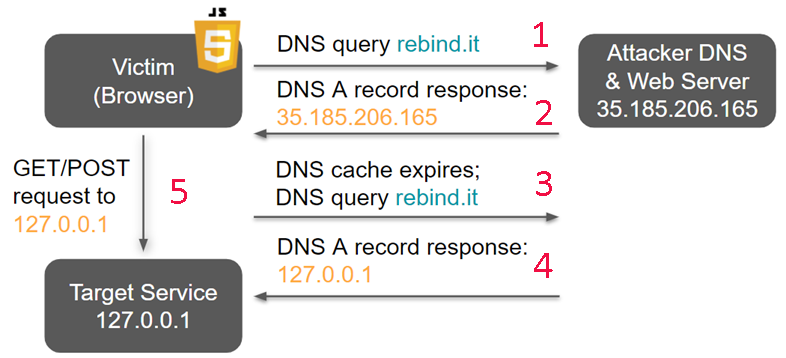
\includegraphics[scale=0.35]{images/DNS_Rebind_Attack.png} 
\caption{Ablauf eines DNS Rebinding Angriffs mittels des des Webtools der NCC Group (\protect\url{http://rebind.it:8080/manager.html} \cite{GeraldDoussot.2019}}
\label{fig:DNS Rebinding Angriff}
\end{center}
\end{figure}


\subsection{Denial of Service Angriff}
\label{dos}
Bei einem \glqq Denial of Service (DoS)\grqq{} Angriff generiert ein Angreifer unzählige Anfragen oder eine sehr große Menge Daten auf einem anderen System, um die Netzwerk- oder \mbox Rechenkapazitäten des Opfers auszuschöpfen. Während eines solchen Angriffes wird der Zugriff auf die Webseite, den Dienst oder den Rechner für legitime Nutzer verhindert \cite{radware.2015} \cite[p.~217]{Fischer.2011}. Es handelt sich also um einen Angriff auf das Schutzziel der Verfügbarkeit.

\begin{quote}
\grqq More simply, a DoS attack is when an attacker uses a single machine’s resources to exhaust those of another machine, in order to prevent it from functioning normally \cite{radware.2015}.\grqq
\end{quote}

\noindent Es handelt sich also bei DoS um ein System, welches ein anderes oder mehrere andere Systeme angreift. Diese Art von Angriff kann entweder durch eine Sicherheitslücke in einem gegebenen System ausgeführt werden, oder über eine Überlastung des Netzwerkes mit Anfragen. Daher teilt man DoS-Attacken meist in drei Kategorien ein \cite{StefanoAlbrecht.2005}:
\end{onehalfspace}

\begin{itemize}
 \item Bandbreitensättigung
 \item Ressourcensättigung
 \item Herbeiführung von System- und Anwendungsabstürzen
\end{itemize}

\begin{onehalfspace}

\noindent Bandbreitensättigung beschreibt das Vorgehen einen Webdienst oder Webserver mit einer großen Menge an Anfragen zu belasten, sodass legitime Nutzer den Dienst nicht, oder nur sehr langsam, nutzen können. Ressourcensättigung ist das Äquivalent für ein gesamtes Rechnersystem. Hier wird eine Sicherheitslücke oder ein Programmierfehler genutzt, um durch einen Prozess eine sehr hohe Auslastung des Systems zu erzeugen, sodass dieses nicht mehr reagiert. Die letzte Art beschreibt das Herbeiführen von Abstürzen. Auf diese Weise kann der Zugriff auf ein Webdienst oder System vollständig unterbrochen werden. Darüber hinaus ist es so möglich, gezielt Elemente eines Netzwerkes wie eine Firewall auszuschalten, sodass ein weiterführender Angriff möglich ist \cite{BundesamtfurSicherheitinderInformationstechnik.2020}.\\
\indent Die meisten Webserver können jedoch Überlastungsversuchen von einem einzelnen System widerstehen. Daher nutzen Angreifer meist mehrere Systeme, welche ein Ziel überlasten sollen. Dies bezeichnet man als \glqq Distributed Denial of Service\grqq{}(DDoS) Angriff \cite[p.~210]{Fischer.2011}. Für diesen Zweck werden in den meisten Fällen viele Systeme unter ein Kommando gestellt, sodass der Angriff koordiniert ablaufen kann. Dies wird als \glqq Botnetz\grqq{} bezeichnet. Den Teilnehmern eines solchen Botnetzes ist oft gar nicht bekannt, dass ihre Geräte durch speziell präparierte Malware infiziert und zu einem Botnetz hinzugefügt wurden \cite{StephenHilt.2020}. Der Einsatz von infizierten IoT-Geräten wird ebenfalls immer beliebter, da diese oft sehr schlecht abgesichert sind und die Nutzer zumeist das Standardpasswort nicht ändern \cite{BSI.2016}.\\
\indent Mögliche Motive für DoS und DDoS sind finanzielle Ziele, politische Motivation (\glqq Hacktivismus\grqq ), zielgerichtete Angriffe auf kritische IT-Infrastruktur oder vertrauliche Daten (\glqq Advanced Persistent Threats\grqq ) sowie Cyberkrieg \cite[p.~12]{radware.2015} \cite{BundesamtfurSicherheitinderInformationstechnik.2020}. DoS und DDoS Angriffe auf Router sind durch die Schnittstellenfunktion des Routers relativ einfach möglich. Die Abwehr solcher Attacken auf Router ist jedoch in den meisten Fällen durch Software und einige Firewall-Regeln automatisch möglich. So kann z.B. die erlaubte Datenrate dynamisch vom Router eingestellt werden, wenn bestimmte Muster in den Anfragen erkannt werden, welche auf einen (D)DoS Angriff hindeuten \cite{StefanoAlbrecht.2005}.



\end{onehalfspace}


\section{Was ist OpenWrt?}
\label{OpenWrt}
\begin{onehalfspace}
OpenWrt (Open Wireless RouTer) ist ein quelloffenes Netzwerk-Betriebssystem für Router, welches auf GNU/Linux basiert und durch eine GNU General Public License (GPL) lizensiert ist \cite{OpenWrtWebseite.}. Die Installation umfasst einen Bootloader, einen Linux-Kernel, ein eigenes Dateisystem und ausgewählte Anwendungen. Es kann auf Routern, Switches und Wireless Access Points eingesetzt werden, um die vorinstallierte Firmware vollständig zu ersetzen \cite{OpenWrtWebseite.16.10.2020}. Es bietet neben standardmäßiger Router-Funktionalität einen eigenen Paketmanager, über welchen ca. 3800 (Stand 01.11.20) weitere Pakete installiert werden können \cite{OpenWrtWebseite.2020}. Dies bietet viele weitere Einsatzmöglichkeiten und Funktionen, welche vom Hersteller nicht oder unzureichend unterstützt werden. Ebenfalls beinhaltet die Installation von OpenWrt den SSH-Dienst BusyBox und das Web-Interface LuCI, sodass dem Nutzer über den root-Benutzeraccount vollständiger Zugriff auf das Gerät gewährt wird. Nach derzeitigem Stand werden über 1700 Geräte von ca. 270 Herstellern von OpenWrt unterstützt \cite{OpenWrtWebseite.18.01.2020}. Diese Anzahl Geräte kann unter anderem deshalb unterstützt werden, da OpenWrt nur minimale Ressourcen auf dem Endgerät benötigt. Nach eigenen Angaben kann die derzeitige Version auf Geräten installiert werden, welche 4MB Flash Speicher und 32MB RAM besitzen. Ab der nächsten \glqq Major Release\grqq{} Version (20.XX) werden 8MB Flash und 64MB RAM vorausgesetzt \cite{OpenWrtWebseite.18.01.2020}. Diese Voraussetzungen sind jedoch bei den meisten Geräten der letzten Jahre gegeben. OpenWrt zeichnet sich ebenfalls dadurch aus, dass es sich nicht nur um eine statische Firmware handelt, sondern ebenfalls um ein komplettes Framework zur Entwicklung und Erstellung von angepassten Firmware Versionen. OpenWrt zeichnet sich auch dadurch aus, dass Geräte solange unterstützt werden, wie sie die minimalen Systemanforderungen erfüllen. Dies steht im Gegensatz zu den meisten proprietären Betriebssystemen, welche nur einige Jahre Funktions- und Sicherheitsupdates erhalten und nach ihrem sog. "`End of Life“ (EOL) nicht mehr sicher betrieben werden können und ausgetauscht werden müssen. Auch wenn in der Entwicklungsgeschichte von OpenWrt viel für die Benutzerfreundlichkeit des Betriebssystems getan wurde, ist es nicht unbedingt für Laien geeignet. Trotz des Managements über die Weboberfläche erweist sich die Einrichtung ohne Grundkenntnisse als anspruchsvoll.\\
  \indent Die Entwicklung von OpenWrt begann 2004, nachdem der amerikanische Hersteller Linksys zuvor einen Router auf den Markt brachte, dessen Firmware zu Teilen ebenfalls unter der GPL Lizenz stand und somit öffentlich verfügbar sein musste. Die erste Veröffentlichung von OpenWrt erfolgte im Januar 2006 mit Version 0.9 (White Russian). Seitdem wurde das Projekt stetig weiterentwickelt (siehe Abbildung \ref{fig:OpenWrt Commits pro Monat}). 2016 spaltete sich eine Gruppe Mitwirkender aufgrund interner Diskrepanzen ab und gründete das LEDE Projekt. Jedoch wurde LEDE bereits 2018 wieder in OpenWrt integriert, sodass beide Projekte nun wieder zusammen unter einem Namen entwickelt werden. Die derzeit aktuelle Version ist 19.07.5, welche am 09.12.2020 veröffentlicht wurde (vergleiche Anhang \ref{tab:OpenWrt_History}) \cite{OpenWrtWebseite.13.12.2020}.\newline

\begin{figure}[ht]
\begin{center}
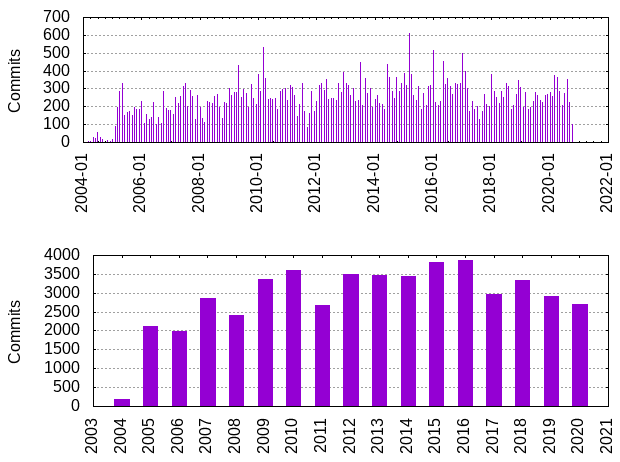
\includegraphics[scale=0.5]{images/commits_by_year_month.png} 
\caption{Die git Commits pro Monat (oben) und pro Jahr von 2004 bis 2020 (unten) des OpenWrt git Repositories. Seit 2005 werden jedes Jahr mindestens 2000 Commits gemacht. Die Grafik wurde mit dem Programm GitStats erstellt (http://gitstats.sourceforge.net).}
\label{fig:OpenWrt Commits pro Monat}
\end{center}
\end{figure}

\end{onehalfspace}

\section{Relevanz und Verwendung von OpenWrt}
\label{OpenWrt Relevanz}
\begin{onehalfspace}
Die Webseite des OpenWrt Projektes verzeichnete im Jahre 2020 bis einschließlich November 1.261.500 Besucher, sowie 52,4 Millionen Seitenaufrufe. Insgesamt wurden bis November 2020 bereits 16,44TB Daten abgerufen \cite{OpenWrtWebseite.29.11.2020}. Die zum Zeitpunkt des Seitenaufrufes aktuelle Version von OpenWrt (19.07.4) wurde dabei allein im November 1981 Mal heruntergeladen. Ebenfalls wurde Version 18.06.8 noch 935 Mal angefragt. Zusammen wurden ca. 10000 Firmware-Abbilder im November 2020 heruntergeladen \cite{OpenWrtWebseite.29.11.2020}. Wie die Daten zeigen ist OpenWrt keinesfalls ein kleines Projekt mit nur wenigen Interessierten, sondern eine nachgefragte Alternative für Heimrouter, Unternehmen und Entwickler. Es lässt sich nur schwer abschätzen wie die Verteilung zwischen dem privaten und wirtschaftlichen Einsatz der Firmware genau ist, jedoch ist eine mehrheitliche Nutzung im privaten Umfeld zu vermuten, da die Downloadzahlen eine Tendenz zu Geräten mit einer günstigeren MIPS-Architektur, anstelle von professionellen Geräten, zeigen (siehe Abbildung \ref{fig:OpenWrt Target}). OpenWrt ist dennoch nicht nur für Heimrouter relevant, sondern zeichnet sich auch in seinem Nutzen für Unternehmen und Entwickler aus. Es bietet Unternehmen die Möglichkeit ein Netz zu betreiben, welches sie vollständig mit quelloffener Software realisieren und steuern können. Ebenfalls bietet es Dienstleistungsunternehmen einen Weg, hochgradig maßgeschneiderte Netzstrukturen für ihre Kunden zu entwerfen, welche quelloffen und leicht anpassbar sind. So können neue oder geänderten Funktionen über ein Paket bereitgestellt und verteilt werden. \newline

\begin{figure}[htb]
\begin{center}
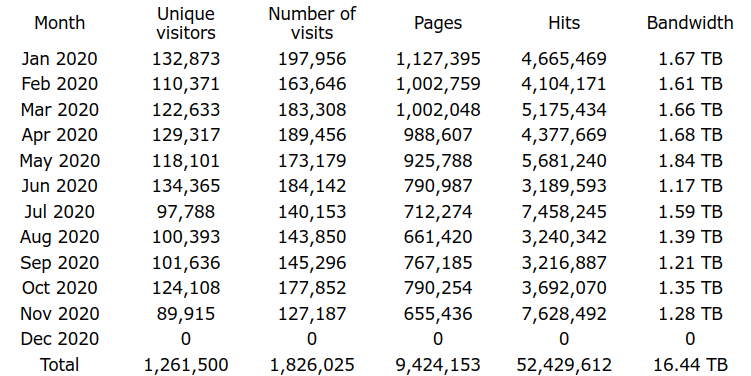
\includegraphics[scale=0.6]{images/openwrt_downloads.png} 
\caption{Übersicht über verschiedene Statistiken der OpenWrt Webseite für das Jahr 2020. (Erstellt: 30.11.2020)}
\label{fig:OpenWrt Webseiten Statistik im Jahr 2020 (ohne Dezember)}

\vspace{0.2cm}

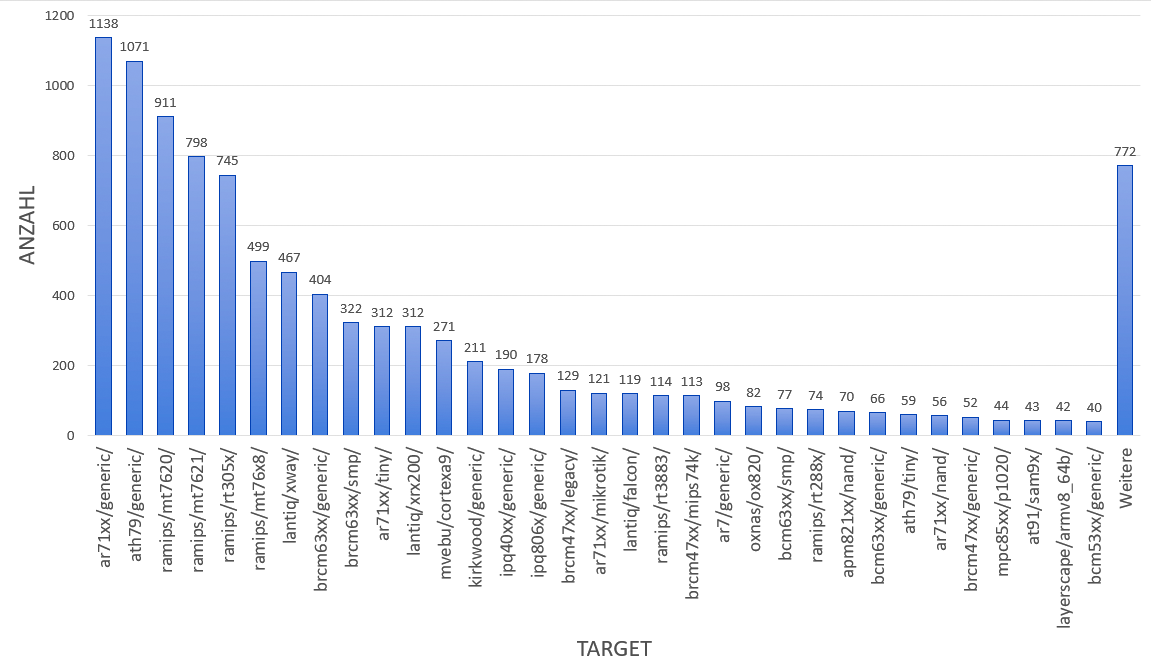
\includegraphics[scale=0.45]{images/openwrt_targets} 
\caption{Anzahl der heruntergeladenen Firmware pro Target im November 2020. Es zeichnet sich ein deutlicher Trend zu günstigeren MIPS-Geräten ab.}
\label{fig:OpenWrt Target}
\end{center}
\end{figure}


\end{onehalfspace}



\section{Möglichkeiten zur Evaluation von Router Firmware}
\label{Router Eval}



\subsection[TR 03148 - Sichere Breitband Router]{Beschreibung der Technischen Richtlinie 03148 - Sichere Breitband Router}
\label{TR}
\begin{onehalfspace}
Bei der Technischen Richtlinie "`Sichere Breitband Router“ (BSI TR-03148) des Bundesamtes für Sicherheit in der Informationstechnik handelt es sich um eine Sammlung von grundlegenden Sicherheitsanforderungen für Breitband Router \cite[p.~3]{BundesamtfurSicherheitinderInformationstechnik.2020b}. Der Schwerpunkt der Richtlinie liegt hierbei vor allem auf Heimroutern, sowie auf Geräten, welche im SOHO Umfeld eingesetzt werden. Das Dokument wird durch die Dokumente "`BSI TR-03148 Implementation Conformance Statement (ICS)“ sowie "`BSI-TR-03148-P ICS and Test Documentation” ergänzt. In diesen Dokumenten sind Testfälle und Dokumentation zur Durchführung einer Prüfung festgehalten. Die Test Spezifikation der Technische Richtlinie definiert 101 "`Test Requirements"{}, welche insgesamt 164 "`Test Procedures"{} beschreiben. Die \glqq Test Requirements\grqq{} sind dabei in logische Module unterteilt. Ein \glqq Test Requirement\grqq{} wird als fehlgeschlagen gewertet, wenn ein zugehöriges \glqq Test Procedure\grqq{} nicht bestanden wird. Nach Angaben des BSI richtet sich die Technische Richtlinie vor allem an Hersteller von Routern, sie kann jedoch auch für Endnutzer relevant sein, wenn diese einen neuen Router anschaffen möchten und sich daher über den Stand der Technik informieren wollen \cite{BundesamtfurSicherheitinderInformationstechnik.e}. Es werden Anforderungen für ein Mindestmaß an verpflichtenden und einigen optionalen IT-Sicherheitsmaßnahmen definiert, um ein grundlegendes Niveau für die Sicherheit dieser Geräte zu schaffen \cite[p.~11]{BundesamtfurSicherheitinderInformationstechnik.2020b}. Die angestrebte Zertifizierung von Geräten würde ebenso die Sicherheit der Geräte für den Verbraucher transparenter machen.	\newline \indent
 	Das Dokument entstand aus einer Zusammenarbeit des BSIs mit verschiedenen Herstellern von Routern, Telekommunikationsanbietern, Behörden, dem Innen- und Wirtschaftsministerium, sowie unter anderem mit Vertretern des OpenWrt Projektes und des Chaos Computer Clubs (CCC) \cite{UlrichHottelet.16.11.2018}. Diese trugen ihre Ideen und Vorstellungen zur Sicherheit von Routern zusammen und suchten Lösungen für Interessenkonflikte. Nach Veröffentlichung der Richtlinie im Jahre 2018 wurde diese allerdings unter anderem von Vertretern des OpenWrt Projektes sowie vom CCC kritisiert. Nach Meinung dieser Interessengruppe sind die definierten Maßnahmen in der Technischen Richtlinie nicht ausreichend, um tatsächliche Angriffe auf Router zu verhindern \cite{CCCundOpenWRTkritisierenRouterTRalsFarce.19.11.2018}.\\
\indent Der Aufbau der Technischen Richtlinie, des \glqq Conformance Statements\grqq{} und der Test Spezifikation ist für das Verständnis der Arbeit unabdingbar. Die Technische Richtlinie selbst beginnt mit einer Beschreibung für welche Geräte die TR genutzt werden soll. Darauf folgt eine Beschreibung des Rahmens, welcher durch die TR vorgegeben wird. So wird festgelegt, dass Router mit einem Betriebssystem betrachtet werden sollen, welche die Schnittstelle zum Internet darstellen und dem Nutzer das Management seines eigenen privaten Netzes ermöglichen. Weiterführend wird festgelegt, dass die Sicherheit von zusätzlichen angeschlossenen Geräten und nicht essenziellen zusätzlichen Funktionsmerkmalen nicht betrachtet wird. Anschließend werden drei Zustände definiert, in dem sich ein Gerät während des Testens befinden kann: \glqq factory settings\grqq , \glqq initialized (after initialization)\grqq{} und \glqq (end user) customized\grqq{} (vgl. Abschnitt \ref{Test Doku}). Bevor die einzelnen logischen Themenmodule der TR erläutert werden, wird zunächst das Bedrohungsmodell definiert (siehe Grafik \ref{fig:threat}). Hierzu werden zwei verschiedene Angreifer festgelegt. Angreifer A greift den Router über das Internet, also die \glqq Wide Area Network\grqq{} (WAN)  Schnittstelle des Routers an, während Angreifer B einen Angriff über das \glqq Local Area Network\grqq{} (LAN) und \glqq Wireless-Lan\grqq{} (WLAN) Interface versucht. An dieser Stelle wird auch ein erweiterter kombinierter Angriff betrachtet. Darauffolgend werden die Module der Technischen Richtlinie beschrieben, welche die Anforderungen in logische Einheiten bündeln. Es werden die folgenden Module beschrieben:
\end{onehalfspace}

\begin{table}[ht]
\centering
\begin{tabular}{lcl}
Module A & - & Private Network (privates Netzwerk)                             \\
Module B & - & Public Network (öffentliches Netzwerk)                          \\
Module C & - & Functionalities (Funktionen)                                    \\
Module D & - & Configuration and Information (Konfiguration und Informationen) \\
Module E & - & Firmware Updates                                                \\
Module F & - & Firewall                                                        \\
Module G & - & Domain Name System (DNS)                                        \\
Module H & - & Dynamic Host Configuration Protocol (DHCP)                      \\
Module I & - & Factory Reset (Zurücksetzen des Gerätes)                        \\
Module J & - & Internet Protocol version 6 (IPv6)                              \\
Module K & - & Remote Configuration (Fernwartung)                              \\
Module L & - & Voice over IP (VoIP)                                            \\
Module M & - & Virtual Private Network (VPN)                                  
\end{tabular}
\end{table}

\begin{onehalfspace}

\begin{figure}[ht]
\begin{center}
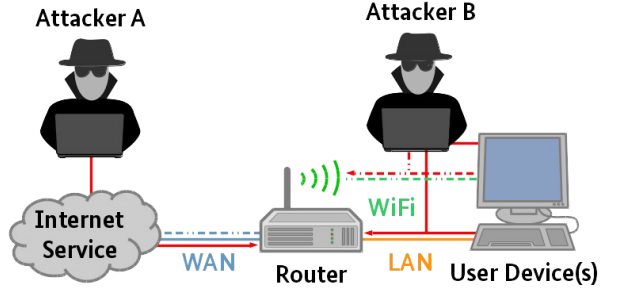
\includegraphics[scale=0.5]{images/threat.png} 
\caption{Das von der Technischen Richtlinie betrachtete Bedrohungsmodell \cite{BundesamtfurSicherheitinderInformationstechnik.e}}
\label{fig:threat}
\end{center}
\end{figure}


Bevor die eigentlichen Tests, welche in der TR beschrieben sind, durchgeführt werden können, muss zunächst ein sogenanntes "`Implementation Conformance Statement“ ausgefüllt werden. In diesem werden maßgebende Informationen über das zu testende Gerät festgehalten. Bei einer Durchführung der Technischen Richtlinie im Kontext einer Zertifizierung würde dieses \glqq Conformance Statement\grqq{} zunächst vom Hersteller bzw. Auftraggeber ausgefüllt und eingereicht. Die angegebenen Informationen unterstützen den Tester, sind aber auch selbst Teil der Testprozedur. Zu diesen Informationen gehören neben dem Namen und der betrachteten Software-Version auch eine Übersicht über die zur Verfügung stehende Dokumentation des Gerätes. Hierzu wird auch technische Dokumentation gezählt, welche normalerweise nicht für Endnutzer und Verbraucher zur Verfügung steht. Des Weiteren werden Informationen zu allen Modulen zusammengetragen, welche bei der Durchführung der \glqq Test Procedures\grqq{} von Relevanz sind. \\ \indent
Der Aufbau der Test Spezifikation orientiert sich ebenfalls an den einzelnen Modulen. Nach einer Einleitung wird zunächst das \glqq Device Under Testing\grqq{}(DUT) beschrieben sowie Ansprüche an die Fähigkeiten und die Ausstattung des Testers. Darauf steht erneut das komplette \glqq Conformance Statement\grqq{} zur Verfügung. Im Anschluss darauf werden die Testfälle, sowie die Kriterien zum Bestehen der Testfälle definiert. Die Ergebnisse können in der Test Dokumentation, welche als Tabellenkalkulationsdatei ausgefüllt wurde, dokumentiert werden. Die Testdokumentation definiert die folgenden Kategorien: Eine durchlaufende Nummerierung und eine Angabe, ob es ein „muss“ oder „soll“ Kriterium ist, eine Beschreibung des Testfalls und die Angabe des Testers, ob der Testfall anwendbar ist oder nicht. Ebenso steht „N/A“ (not applicable) als Option zur Verfügung. Darauf folgen Felder für die jeweiligen Ergebnisse der Tests einer jeden Testreihe, gefolgt von der Möglichkeit für Notizen, Referenzen, benutze Tools, Zugriffsmethoden und einer Referenz für weitere Daten wie Bilder (siehe Tabelle \ref{tab:TR}).


\begin{table}[ht]
\def\arraystretch{1.5}
\centering
\resizebox{\textwidth}{!}{%
\begin{tabular}{lll|l|l|l|lllllllll}
\cline{1-6}
\multicolumn{1}{|l|}{\textbf{TR}} &
  \multicolumn{1}{l|}{\textbf{\begin{tabular}[c]{@{}l@{}}MUST or\\ SHOULD\end{tabular}}} &
  \textbf{\begin{tabular}[c]{@{}l@{}}Description\\ of TR\end{tabular}} &
  \multicolumn{3}{l|}{\textbf{\begin{tabular}[c]{@{}l@{}}Applicability of Test   \\      Requirements\end{tabular}}} &
   &
   &
   &
   &
   &
   &
   &
   &
   \\ \hline
 &
   &
   &
  Yes &
  No &
  N/A &
  \multicolumn{1}{l|}{1. TP} &
  \multicolumn{1}{l|}{2. TP} &
  \multicolumn{1}{l|}{3. TP} &
  \multicolumn{1}{l|}{4. TP} &
  \multicolumn{1}{l|}{5. TP} &
  \multicolumn{1}{l|}{Notes} &
  \multicolumn{1}{l|}{\begin{tabular}[c]{@{}l@{}}Used \\ Tools\end{tabular}} &
  \multicolumn{1}{l|}{\begin{tabular}[c]{@{}l@{}}Used \\ Configuration\\ Access Method\end{tabular}} &
  \multicolumn{1}{l|}{\begin{tabular}[c]{@{}l@{}}Test data \\ reference\end{tabular}} \\ \hline
\multicolumn{15}{|l|}{\textbf{Module   A - Private Network}} \\ \hline
\multicolumn{1}{|l|}{TR.A.1} &
  \multicolumn{1}{l|}{MUST} &
  ... &
  X &
   &
   &
  \multicolumn{1}{l|}{\cellcolor[HTML]{32CB00}Pass} &
  \multicolumn{1}{l|}{\cellcolor[HTML]{FE0000}Fail} &
  \multicolumn{1}{l|}{\cellcolor[HTML]{F8FF00}Inc.} &
  \multicolumn{1}{l|}{\cellcolor[HTML]{C0C0C0}N/A} &
  \multicolumn{1}{l|}{} &
  \multicolumn{1}{l|}{} &
  \multicolumn{1}{l|}{nmap} &
  \multicolumn{1}{l|}{web-interface} &
  \multicolumn{1}{l|}{1.png} \\ \hline
\multicolumn{1}{|c|}{\begin{tabular}[c]{@{}c@{}}.\\ .\\ .\end{tabular}} &
  \multicolumn{1}{l|}{} &
   &
   &
   &
   &
  \multicolumn{1}{l|}{} &
  \multicolumn{1}{l|}{} &
  \multicolumn{1}{l|}{} &
  \multicolumn{1}{l|}{} &
  \multicolumn{1}{l|}{} &
  \multicolumn{1}{l|}{} &
  \multicolumn{1}{l|}{} &
  \multicolumn{1}{l|}{} &
  \multicolumn{1}{l|}{} \\ \hline
\multicolumn{15}{|l|}{\textbf{Module B - Public Network}} \\ \hline
\multicolumn{1}{|c|}{\begin{tabular}[c]{@{}c@{}}.\\ .\\ .\end{tabular}} &
  \multicolumn{1}{l|}{} &
   &
   &
   &
   &
  \multicolumn{1}{l|}{} &
  \multicolumn{1}{l|}{} &
  \multicolumn{1}{l|}{} &
  \multicolumn{1}{l|}{} &
  \multicolumn{1}{l|}{} &
  \multicolumn{1}{l|}{} &
  \multicolumn{1}{l|}{} &
  \multicolumn{1}{l|}{} &
  \multicolumn{1}{l|}{} \\ \hline
\multicolumn{15}{|l|}{\textbf{Module C - Functionalities}} \\ \hline
\multicolumn{1}{|c|}{\begin{tabular}[c]{@{}c@{}}.\\ .\\ .\end{tabular}} &
  \multicolumn{1}{l|}{} &
   &
   &
   &
   &
  \multicolumn{1}{l|}{} &
  \multicolumn{1}{l|}{} &
  \multicolumn{1}{l|}{} &
  \multicolumn{1}{l|}{} &
  \multicolumn{1}{l|}{} &
  \multicolumn{1}{l|}{} &
  \multicolumn{1}{l|}{} &
  \multicolumn{1}{l|}{} &
  \multicolumn{1}{l|}{} \\ \hline
\end{tabular}%
}
\caption{Aufbau der Test Dokumentation als Tabellenkalkulationsdatei.}
\label{tab:TR}
\end{table}


\end{onehalfspace}


\subsection{Statische Softwaretests}
\label{Softwaretests}
\begin{onehalfspace}
Bei einem statischen Softwaretest wird die Software nicht während der Laufzeit (vgl. dynamischer Softwaretest) getestet, sondern der eigentliche Quellcode oder der dekompilierte Bytecode analysiert. Statische Softwaretests gehören also zur Gruppe der sog. \glqq non-execution-based\grqq -Methoden. Dynamische Softwaretests bezeichnet man hingegen als \glqq execution-based\grqq , da die Software ausgeführt werden muss. Zu den statischen Softwaretests gehören unter anderem das Software-Review oder auch werkzeuggestütze automatische Verfahren. Wie die meisten Softwaretestverfahren gehören statische Softwaretests zu den falsifizierenden Verfahren und können somit lediglich die Anwesenheit von Fehlern bestimmen \cite{Spillner.2019, Myers.2012}. \\ \indent
Bei einem Software-Review wird der Quellcode, die Dokumentation oder jedes weitere Dokument eines Softwareentwicklungsprozesses von einem oder mehreren Prüfern inspiziert und ausgewertet. Dabei sollte nach einen festgelegten Plan vorgegangen werden. Darüber hinaus müssen auch psychologische Effekte in Betracht gezogen werden, sodass der Entwickler des geprüften Dokumentes sich nicht persönlich kritisiert sieht \cite{Spillner.2019}. \\ \indent
Werkzeuggestützte statische Softwaretests kommen in vielen Formen vor. So führen die meisten integrierten Entwicklungsumgebungen (IDE) und Compiler bereits eine statische Analyse durch. Sie zeigen z.B. Abweichungen von voreingestellten Code-Stilen an, sodass ein Entwickler darin unterstützt wird, einheitlichen und strukturierten Code zu schreiben. Ebenso werden sog. \glqq Code Smells\grqq{} in einigen IDEs angezeigt. Es handelt sich hierbei um ein Code-Konstrukt oder Code-Abschnitt, welcher es nahelegt, diesen zu refaktorisieren. Dazu gehören zum Beispiel Duplikate im Quellcode oder zu lange und komplexe Methoden. Viele moderne IDEs zeigen noch viele Metriken zur Verbesserung des Quellcodes an \cite{Spillner.2019, Mili.2015}. Es existieren jedoch auch Programme, mit denen gezielt eine statische Analyse durchgeführt werden kann. Ein Beispiel hierfür ist das Programm \glqq Lint\grqq . Es ist eines der ersten Programme für statische Softwaretests und prüfte kritische Stellen, wie nicht initialisierte Variablen, da dies von frühen Compilern nicht unterstützt wurde \cite{Johnson1978LintAC}. Ein weiteres bekanntes Beispiel ist das \glqq Rough Auditing Tool for Security\grqq{}(RATS) Programm. Es unterstützt mehrere Programmiersprachen und prüft viele verschiedene Fehler \cite{SecureSoftwareInc..2013}. Jedoch müssen die Ergebnisse dieser Programme aufgrund einer erhöhten Falsch-Positiven-Rate von einem Menschen kontrolliert werden.
\end{onehalfspace}



\subsubsection{Firmware Analysis and Comparison Tool}
\label{FACT}
\begin{onehalfspace}
Das \glqq Firmware Analysis and Comparison Tool\grqq{} (FACT) ist ein quelloffenes Programm zur statischen Analyse von Firmware, welches vom Fraunhofer-Institut für Kommunikation, Informationsverarbeitung und Ergonomie entwickelt wurde. Es ist in der Lage arbiträre Firmware (Router, Webcams, UEFI, etc.) zu entpacken und mehrere Analysen durchzuführen. Nachdem mehrere Firmware-Abbilder extrahiert und analysiert wurden, kann FACT ebenfalls genutzt werden, um diese miteinander zu vergleichen. Eine Benutzeroberfläche wird dabei durch ein Web-Interface bereitgestellt, während die eigentliche Funktionalität über Plug-Ins organisiert ist, sodass eigens entwickelte Komponenten einfach hinzugefügt werden können. FACT automatisiert somit den normalerweise aufwendigen Prozess der Firmware-Analyse \cite{FraunhoferFKIE.2020}. In der Standardinstallation stellt FACT die folgenden Plug-Ins für die Analyse zur Verfügung:
\end{onehalfspace}

\begin{itemize}
\setlength\itemsep{0.03em}
\item Identifikation der Software
\begin{itemize}
\item Betriebssystem erkennen
\item Welche Programme sind installiert?
\item Welche Programmversionen kommen zum Einsatz?
\item Welche Routinen werden beim Systemstart gestartet?
\item Können bekannte Schwachstellen gefunden werden?
\end{itemize}
\item Benutzerkonten finden. Vor allem hartkodierte Passwörter
\item Kryptographisches Material identifizieren
\begin{itemize}
\item Private Schlüssel
\item Zertifikate
\end{itemize}
\item CPU-Architektur bestimmen (Für Emulation und Disassembler)
\item QEMU Unterstützung evaluieren (Für Debugging und Fuzzing)
\item Bekannte Fehler in der Implementierung
\item Exploit Mitigationen auswerten
\item zusätzliche Plug-Ins
\end{itemize}
 


\subsubsection{Härtungsmaßnahmen}
\label{Hardening}
\begin{onehalfspace}

FACT ist in der Lage einige bekannte Härtungsmaßnahmen (auch als Exploit Mitigationen bezeichnet) für elf-Binärdateien in einem Firmware-Abbild zu analysieren. So kann angezeigt werden welche Binärdateien mit diesen Maßnahmen erzeugt wurden und welche nicht. Diese Härtungsmaßnahmen sind vor allem Wege zur Mitigation von Speicherkorruption, entweder durch einen Angreifer oder durch Systemfehler. FACT kann folgende Mitigationen auswerten:

\begin{itemize}
\item \textbf{Stack Canary}: Es handelt sich hierbei um eine zufällig gewählte Byte-Sequenz, welche vor die "`return“-Adresse auf den Stack geschrieben wird, um Overflows zu erkennen. Diese zufällige Sequenz wird aus einer statisch adressierbaren Speicherregion außerhalb des Stacks geholt \cite{RubenGonzalez.29.04.2019}. Wenn es zu einem Buffer-Overflow kommt, würde diese Sequenz überschrieben und diese kann somit nicht vor dem Zurückkehren (return) verifiziert werden, sodass der Overflow erfolgreich erkannt wird \cite{xorl.2010}. Wenn die Werte nicht übereinstimmen, dann wird eine Kernel-Panik ausgelöst und der Prozess terminiert. 

\item \textbf{FORTIFY\_SOURCE} ist eine zusätzliche Option der GCC Compiler Collection. Wenn diese Option beim Kompiliervorgang von Dateien ausgewählt wird, werden verschiedene Funktionen zur Manipulation von Zeichenketten und Speicher (memcpy, memset, strcpy, strcat, sprintf, gets, ...) während der Ausführung auf Pufferüberläufe (buffer overflow) geprüft. Dies schützt meistens nicht vor gezieltem Ausnutzen dieser Funktionen aber vor der Korruption des Heaps und Stacks durch Systemfehler \cite{SiddharthSharma.2014}.  

\item \textbf{Non-Executable Bit (NX)}: Dieses besondere Bit markiert Bereiche des Speichers als reine Datenspeicherbereiche. Dadurch wird sichergestellt, dass in diesen Bereichen, in denen kein Code ausgeführt werden sollte, auch kein Code ausgeführt werden kann. Diese Separierung findet sich sonst nur in Harvard-Architekturen \cite[p.~11]{PeterWeidenbachJohannesvomDorp.2020}.

\item \textbf{Position-Independent Executable (PIE)} (positionsunabhängiges ausführbares Programm) bezeichnet eine Technik, bei welcher Programm-Code an einer zufälligen \mbox Speicheradresse geladen wird. Hierbei wird nicht mit absoluten, sondern relativen Speicheradressen gearbeitet. Dies erschwert zwar Angriffe, da ein Angreifer zunächst die absolute Speicheradresse finden muss, jedoch verlangsamt diese Technik unter Umständen auch die Ausführung des Codes \cite{Payer.2012}. 

\item \textbf{RELocation Read-Only (RELRO)} schützt den “Global Offset Table” (GOT) gegen Manipulationen während der Laufzeit. Der Global Offset Table beinhaltet die \mbox Speicheradressen von gemeinsam genutzten Softwarebibliotheken oder globalen \mbox Variablen, sodass diese von einem Programm genutzt werden können. Wenn die \mbox RELRO Option beim Kompiliervorgang ausgewählt wurde, dann wird nach dem Start des Programms ein reiner Lesezugriff auf den GOT festgelegt \cite[p.~12]{PeterWeidenbachJohannesvomDorp.2020}. 

\end{itemize}
\end{onehalfspace}


\subsubsection{Common Vulnerabilities and Exposures}
\label{CVE}
\begin{onehalfspace}
Das \glqq Common Vulnerabilities and Exposures\grqq{}(CVE) System wurde 1999 geschaffen, um ein weltweit einheitliches System zur Beschreibung von Firmware oder Software Schwachstellen zu etablieren \cite{MITRE.2020}. Sogenannte \glqq CVE Numbering Authorities\grqq{}(CNAs) vergeben pro Sicherheitslücke eine spezifische Identifikationsnummer. Nachdem eine Beschreibung und Referenzen formuliert wurden, wird der Eintrag in die CVE-Datenbank aufgenommen und kann weltweit eingesehen werden. Durch das festgelegte Format von CVE-Einträgen ist auch die automatische Verarbeitung von Einträgen möglich. Dies kann für die automatische Notifikation eines Betroffenen genutzt werden, wenn eine sicherheitsrelevante Schwachstelle gemeldet wird. Das CVE Projekt wird von dem US-Amerikanischen Unternehmen \glqq MITRE\grqq{} unterhalten \cite{Luigi.2020}.\\ \indent
Da CVE-Einträge keinen Aufschluss über die schwere der Sicherheitslücke geben, wurde 2005 vom \glqq Forum of Incident Response and Security Teams\grqq{}(FIRST) ein \mbox Bewertungssystem für CVE-Einträge entwickelt. Dieses als \glqq Common Vulnerability \mbox Scoring System\grqq{}(CVSS) bezeichnete System ist heute der Industriestandard \cite{Luigi.2020}. Das CVSS-Bewertungssystem ermöglicht es, die Erarbeitung von Lösungen für Sicherheitslücken zu priorisieren. Jeder CVE-Eintrag erhält durch eine Reihe von Metriken, welche den Anspruch und die Auswirkung einer gegebenen Sicherheitslücke in Betracht ziehen, eine CVSS Bewertung zwischen null und zehn. Eine Bewertung von zehn ist dabei die schwerwiegendste Stufe \cite{CVSS2.2007}. 2007 wurde die zweite Version, CVSS2 (auch CVSS v2), veröffentlicht und 2015 wurde CVSS3 (CVSS v3) herausgegeben \cite{CVSS2.2007, CVSS3.2015}. Die neuste Version beinhaltet überarbeitete Metriken sowie ein neues Einstufungssystem mit zwei neuen Stufen (vgl. Tabelle \ref{tab:CVSS dif}). Die Bewertungen sind nicht mit einander vergleichbar \cite{CVSS3.2015}. Da vor allem ältere Sicherheitslücken keine CVSS3 Bewertung haben, wird im weiteren Verlauf dieser Arbeit das CVSS2 System verwendet.


\begin{table}[ht]
\centering
\begin{tabular}{lcc}
Rating   & \multicolumn{1}{l}{CVSS2 Score} & \multicolumn{1}{l}{CVSS3 Score} \\ \hline
None     & -                               & 0.0                             \\
Low      & 0.0 - 3.9                       & 0.1 - 3.9                       \\
Medium   & 4.0 - 6.9                       & 4.0 - 6.9                       \\
High     & 7.0 - 10.0                      & 7.0 - 8.9                       \\
Critical & -                               & 9.0 - 10.0                     
\end{tabular}
\caption{Unterschiede in der Bewertungsskala von CVSS2 und CVSS3 \cite{CVSS2.2007, CVSS3.2015}}
\label{tab:CVSS dif}
\end{table}
 
\end{onehalfspace}


%###############################################################################

\chapter{Methodik}
\label{methods}

\section{Übersicht und Begründung der verwendeten Methodik}
\label{overview methods}
\begin{onehalfspace}
Die Methodik der Arbeit ist in großen Teilen durch die Technische Richtlinie vorgegeben. Die Testfälle wurden aufgrund ihrer Gruppierung in thematische Module in chronologischer Reihenfolge erarbeitet (siehe Abschnitt \ref{TR}). Einzig solche Testfälle, welche spezifizierten, dass sie erst zum Ende der Testphase durchgeführt werden sollten, wurden nach hinten gestellt. Da es in erster Linie um die Technische Richtlinie 03148 gehen sollte, wurden weitere Tests, wie ein statischer Test mit dem "`Firmware Analysis and Comparison Tool“ (siehe Abschnitt \ref{FACT}), erst nach Vollendung der Technischen Richtlinie begonnen \cite{FraunhoferFKIE.2020}. 	\newline\indent
	Die Testfälle der Technischen Richtlinie wurden, soweit möglich, mit den Programmen durchgeführt, welche in der TR selbst spezifiziert wurden. Die Ergebnisse einer Literaturrecherche zeigten, dass die aufgeführte Software für die Überprüfung der Testanforderungen geeignet ist und die Ergebnisse dieser Programme seit vielen Jahren weitestgehend als korrekt akzeptiert sind. Hierzu zählt vor allem das Programm nmap, welches aufgrund von verschiedenen Testrechnern in den Versionen 7.80, 7.90 und 7.91 verwendet wurde \cite{Lyon.2008}. Die Änderungshistorie von nmap gibt allerdings keinen Anlass zur Annahme, dass dies die Ergebnisse invalidiert \cite{GordonFyodorLyon.2020}. Ebenso wurde airmon-ng / airodump-ng in der Version 1.6 zum Prüfen verwendet. Dieses Softwarepaket ist ebenfalls seit vielen Jahren angesehen und findet in wissenschaftlichen Arbeiten Verwendung \cite{AcostaLopez.2018, Waliullah.2015}. Zur Aufzeichnung von Netzwerkpaketen wurde Wireshark 3.4.2 verwendet, welches neben der Kommandozeilenanwendung tcpdump häufig Verwendung findet \cite{Goyal.16.09.201717.09.2017, Sanders.2017}. Im Rahmen der Tests wurde des Weiteren auf einige zweckspezifische Skripte in den Programmiersprachen Python und Bash zurückgegriffen. Bei der Entwicklung wurde Wert auf einfache Ausführbarkeit, sowie eine geringe Zahl an externen Abhängigkeiten, gelegt, um eine wiederholbare Ausführbarkeit auch in der Zukunft zu gewährleisten. Wireshark und nmap wurden, neben den bereits genannten Gründen, aufgrund der wiederholten expliziten Nennung in der Technischen Richtlinie gewählt. Die verwendeten Programme des Aircrack-ng Softwarepaketes wurden genutzt, da diese auch in den bereits durchgeführten Prüfungen von Geräten durch die TR zum Einsatz kamen. Eine Alternative zu nmap bietet das Programm \glqq MASSCAN\grqq{} oder \glqq Angry IP Scanner\grqq{} \cite{MASSCAN.2020, ANGRYIP.2020}. Jedoch ermöglichen beide Programme nicht den Funktionsumfang von nmap. Vergleichbare Funktionalität zu den Programmen aus dem aircrack-ng Paket hat das \glqq netsniff-ng toolkit\grqq{} \cite{sniff.2020}. Neben tcpdump stellt auch \glqq Ethercap\grqq{} eine geeignete Alternative zu Wireshark dar. So können Netzwerkmitschnitte ebenfalls im \glqq pcap\grqq{} Format gespeichert werden, welches auch Wireshark nutzt \cite{etter.2020}.    \\ \indent
Als Router wurde ein TP-Link Archer C7 (AC1750) Dualband-Gigabit-WLAN-Router (v5) verwendet. Dieses Modell wurde aufgrund der Beliebtheit im OpenWrt-Umfeld, der Verfügbarkeit, der aktuellen Ausstattung und dem Preis-Leistungs-Verhältnis gewählt. Die Statistiken der OpenWrt-Webseite haben gezeigt, dass die zu dem Gerät gehörige Version die am dritthäufigsten heruntergeladene OpenWrt-Firmware im November des Jahres 2020 ist (vgl. Tabelle \ref{tab:downloads}). Bei dem Xiaomi Mi R3P und dem D-Team Newifi D2 Router, welche öfter abgefragt wurden, handelt es sich zwar um günstigere Geräte, allerdings haben diese nur eine eingeschränkte Verfügbarkeit in Deutschland. Die vom gewählten TP-Link unterstützten Funktionen sind darüber hinaus vergleichbar mit vielen Endgeräten, welche im privaten und SOHO Umfeld eingesetzt werden.

\begin{table}[ht]
\centering
\def\arraystretch{1.3}
\resizebox{\textwidth}{!}{%
\begin{tabular}{llll}
 & \textbf{Firmware image}                                                                                         & \textbf{Hits} & \textbf{Bandwidth} \\ \cline{2-4} 
 & /releases/19.07.4/targets/ramips/mt7621/openwrt-19.07.4-ramips-mt7621-xiaomi\_mir3p-initramfs-kernel.bin        & 2598          & 528.26 MB          \\
 & /releases/19.07.4/targets/ramips/mt7621/openwrt-19.07.4-ramips-mt7621-d-team\_newifi-d2-squashfs-sysupgrade.bin & 1289          & 3.90 GB            \\
$\hookrightarrow$ & /releases/19.07.4/targets/ath79/generic/openwrt-19.07.4-ath79-generic-tplink\_archer-c7-v5-squashfs-factory.bin & 1255 & 4.91 GB \\
 & /releases/19.07.4/targets/ath79/generic/openwrt-19.07.4-ath79-generic-tplink\_archer-c6-v2-squashfs-factory.bin & 1129          & 4.27 GB           
\end{tabular}%
}

\caption{Auszug aus den Downloadzahlen pro Firmware vom 30.11.2020.}
\label{tab:downloads}
\end{table}


\end{onehalfspace}

\section{Aufbau und Beschreibung der Testumgebung}
\label{umgebung}
\begin{onehalfspace}
Der genutzte Testaufbau soll einen reibungslosen Ablauf der Testfälle erlauben sowie einfach reproduzierbar sein. Der Internetanschluss wurde durch den Internet Service Provider (ISP) bn:t Blatzheim Networks Telecom GmbH zur Verfügung gestellt. Der Glasfaseranschluss des ISP terminiert in einer FRITZ!Box 5530 Fiber, welche das Subnetz 192.168.178.0/24 bereitstellt. Der WAN Port des mit OpenWrt 19.7.04 bespielten TP-Link Archer C7 v.5 Dualband-Gigabit-WLAN-Router, wurde mit dieser FRITZ!Box verbunden, sodass der OpenWrt-Router das Subnetz 192.168.1.0/24 zur Verfügung stellen konnte. Die Erstinstallation von OpenWrt auf dem TP-Link Router erfolgte über die zur Verfügung stehende Anleitung \cite{OpenWrtWebseite.2019}. Zunächst wurde das Firmware-Abbild heruntergeladen, daraufhin wurden die Hash-Werte mit den veröffentlichten und signierten Hash-Werten abgeglichen. Nachdem sichergestellt wurde, dass diese übereinstimmten, konnte die Datei über das Web-Interface des TP-Link Routers aufgespielt werden. Die OpenWrt Installationsdatei wurde hierzu über die Firmware-Update Funktion hochgeladen und automatisch vom Gerät installiert. Das Gerät startet daraufhin persistent mit OpenWrt anstelle des Betriebssystems von TP-Link. \mbox Alternativ besteht die Möglichkeit das Firmware-Abbild von OpenWrt über die "`Trivial File Transfer Protocol“ (TFTP) Funktionalität des Routers aufzuspielen. \\
\indent Ein Testcomputer wurde über das LAN Interface angeschlossen, ein weiterer Laptop per WLAN und LAN verbunden (siehe Abbildung \ref{fig:Testumgebung TR}). 
Der Testcomputer wurde wahlweise mit Windows 10 Version 20H2 (Build 19042.685) oder Ubuntu 20.04 LTS betrieben. Auf dem Laptop kam Kali Linux 2020.2 zum Einsatz. Dieser Aufbau gibt dem Tester eine flexible Arbeitsumgebung, in welcher die Tests ungestört durchgeführt werden können. Durch die Abtrennung des Netzes in das 192.168.1.0/24 Subnetz durch den OpenWrt Router sind Geräte des allgemeinen Heimnetzes von Portscans und Netzwerkpaketmitschnitten ausgeschlossen. Dadurch können Tests performanter durchgeführt werden, während andere Teilnehmer des Netzes ungestört weiterarbeiten können. Ebenso bietet der beschriebene Aufbau einfach die Möglichkeit weitere Geräte, welche für Tests benötigt werden, hinzuzufügen. Die verwendeten Linux-Distributionen, Ubuntu 20.4 LTS und Kali Linux, bieten die Möglichkeit die notwendigen Programme reibungslos zu betreiben. 

\begin{figure}[ht]
\begin{center}
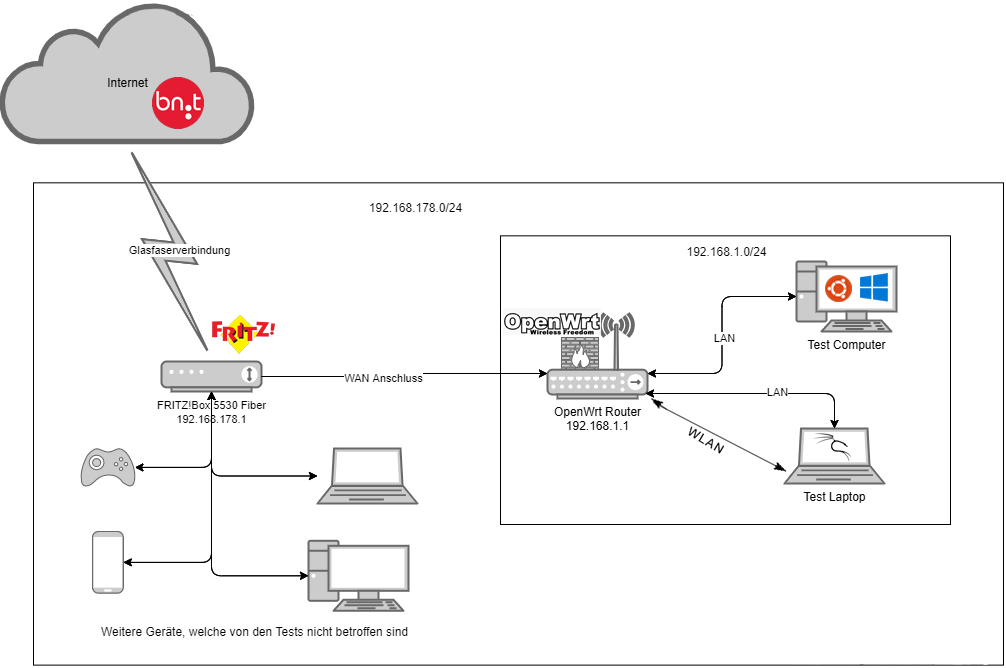
\includegraphics[scale=0.45]{images/testumgebung.png} 
\caption{Aufbau der eingesetzten Testumgebung. Es handelt sich hierbei um einen sog. \glqq double NAT\grqq{} Aufbau, d.h. der OpenWrt-Router hat keinen nativen Internetanschluss sondern bezieht die Internetverbindung über einen vorgelagerten Router. Die Tests wurden im Subnetz 192.168.1.0/24 durchgeführt.}
\label{fig:Testumgebung TR}
\end{center}
\end{figure}

\indent Dieser sogenannte "`double NAT“ (Network Address Translation) Aufbau (vergleiche Abbildung \ref{fig:Double NAT Erklärung}) stellt praktisch keinen Nachteil dar \cite{OpenWrtWebseite.07.12.2020}. Obwohl der direkte Anschluss des OpenWrt-fähigen Routers präferiert eingesetzt werden sollte, können alle Tests ohne Integritätsverlust durchgeführt werden. Die Tests bezüglich des WAN Anschlusses können über die IP-Adresse des OpenWrt Routers durchgeführt werden, welche durch die FRITZ!Box vergeben wurde. Weiterhin wurde der "`Domain Name System Resolver“ (DNS Resolver) der FRITZ!Box auf die IP-Adresse des OpenWrt Routers geändert, um die Tests bzgl. des DNS-Protokolls und der Implementierung nicht zu verfälschen. Alle verfügbaren Firewall- und Filter-Einstellungen der FRITZ!Box wurden ebenfalls während der Tests deaktiviert. 


\begin{figure}[ht]
\begin{center}
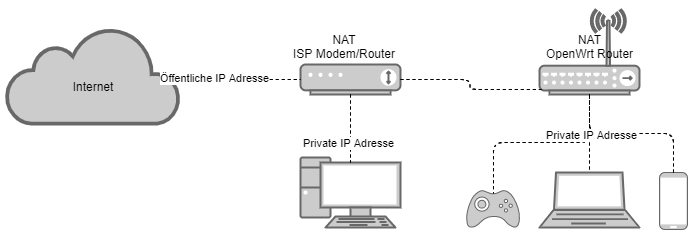
\includegraphics[scale=0.4]{images/Double_NAT} 
\caption{Beispiel einer allgemeinen \glqq double NAT\grqq{} Umgebung. Die Darstellung basiert auf: https://kb.netgear.com/30186/What-is-Double-NAT (abgerufen: 13.12.2020) }
\label{fig:Double NAT Erklärung}
\end{center}
\end{figure}

\end{onehalfspace}

\section{Durchführung der Testfälle}
\label{Testfälle}
\subsection{Conformance Statement}
\label{ICS}
\begin{onehalfspace}
Im Falle dieser Arbeit wurde das \glqq Conformance Statement\grqq{} (vgl. Abschnitt \ref{TR}) als Teil der Richtlinie betrachtet und mit den in der Online-Dokumentation von OpenWrt beschriebenen Informationen ausgefüllt. Darüber hinaus konnte der Quellcode Aufschluss über in der Dokumentation ungeklärte Fragestellungen geben. Die Informationen zu Modul A zeigen, dass OpenWrt eine vergleichsweise geringe Anzahl an Diensten im Ausgangs- sowie initialisierten Zustand anbietet. Lediglich der Web-Server uHTTPd auf Port 80, der SSH Server auf Port 22 und der von dnsmasq zur Verfügung gestellte DNS-Dienst auf Port 53 sind aktiv. Funktionen wie das Session Initiation Protocol (SIP) für Voice-over-IP-Telefonie (vgl. Abschnitt \ref{Router}) oder Protokolle zur externen, automatischen Konfiguration des Geräts, welche oft bei handelsüblichen Routern verwendet werden, fehlen vollends. Ebenso gibt die Dokumentation an, dass das veraltete und als unsicher geltende Wi-Fi Protected Setup (WPS) Verfahren ohne die Installation von zusätzlicher Software nicht verwendet werden kann \cite{StefanViehbock.2011}. Dies ist auf vielen aktuellen Geräten in den Standardeinstellungen aktiviert. Aus dieser eingeschränkten Menge an Diensten wird ersichtlich, dass das Gerät nur über die Netz-Schnittstelle oder per SSH eingerichtet und bedient werden kann. Jedoch steht dem Nutzer standardmäßig der sogenannte "`root“ Benutzer zur Verfügung, sodass uneingeschränkter Zugriff auf alle Funktionen und Einstellungen des Gerätes gewährleistet ist. Eine weitere \mbox Besonderheit zeigt sich in auch in der Vorkonfiguration des WLAN-Netzes von OpenWrt. Dies ist zunächst deaktiviert und wird standardmäßig ohne Passwort initialisiert. Begründen kann man dies damit, dass OpenWrt nicht mit gerätespezifischer Dokumentation ausgeliefert werden kann wie sonst üblich. Ein Schriftstück mit einzigartigem Passwort für das Gerät, sowie das voreingestellte WLAN, kann nicht erstellt werden. So muss jedes Passwort, welches für ein OpenWrt Gerät verwendet wird, vom Benutzer selbst erstellt werden. Dies kann sowohl positive als auch negative Implikationen für die Sicherheit des Gerätes haben. Zum einen verhindert dieses Vorgehen, dass ein Hersteller ein unsicheres Passwort festlegt, welches ein unerfahrener Nutzer nicht ändert. Ebenso könnte der Hersteller ein bestimmtes Muster oder Master-Passwort verwenden. Wenn dieses veröffentlicht wird, so sind alle Geräte auf denen das Passwort nicht geändert wurde in Gefahr. Zum anderen könnte der Nutzer ein unsicheres Passwort vergeben, wenn er damit konfrontiert wird. Wenn vom System keine festen Ansprüche an dieses Passwort gesetzt werden, so würde ein schwaches Passwort die Sicherheit des Gerätes ebenso kompromittieren (siehe Abschnitt \ref{bruteforce}). \newline\indent	
Schon im zweiten Abschnitt des \glqq Conformance Statement\grqq{}, welcher sich auf das öffentliche Netz bezieht, wird erkenntlich, dass auch auf Seiten des Internets nur eine minimale Anzahl an Diensten verwendet wird. Die Dokumentation von OpenWrt spezifiziert keinen Dienst, welcher auf dem WAN-Interface angeboten wird. Ein vergleichbarer Trend kann auch bei den angebotenen Funktionen des Geräts beobachtet werden. Lediglich sehr grundlegende Funktionen wie DHCP, SSH, secure copy (SCP), IPv6 Unterstützung und eine Firewall werden angeboten. Die eigens für OpenWrt entwickelte, quelloffene Packet-Management Software "`opkg“, über welche zusätzliche Funktionalität installiert werden kann, bildet jedoch eine Ausnahme. Der geringe Umfang an Funktionen lässt sich in zweierlei Hinsicht begründen. Durch den Packet Manager opkg kann gewünschte Funktionalität leicht vom Benutzer selbst installiert und eingerichtet werden, ohne schon im Vorhinein Speicherplatz für Funktionen zu nutzen, welche unter Umständen nicht verwendet werden. Darüber hinaus kann OpenWrt so auch auf Geräten mit limitiertem persistenten Speicher oder Arbeitsspeicher installiert werden. So kann zum Beispiel das Web-Interface von der Installation ausgeschlossen sein, wenn ein Gerät nicht über genügend Speicher verfügt. Dadurch ist eine minimale Installation auf Geräten mit 4MB Flashspeicher und 32MB RAM möglich (vgl. Abschnit \ref{OpenWrt}). \newline\indent	
	Ein Defizit von OpenWrt lässt sich jedoch bereits im \glqq Conformance Statement\grqq{} finden. Es besteht keine Möglichkeit sicherheitsrelevante Updates automatisch einzuspielen. Über den Paket Manager bereitgestellte Funktionen könnten zwar mittels sog. CronJobs \mbox aktualisiert werden, dies würde jedoch nur periodisch nach Einstellung des Nutzers geschehen. Dies bietet keine Sicherheit, wenn die Periode zu groß gewählt wurde. Sicherheitslücken im Linux Kernel können jedoch nur über vollständige Firmware-Upgrades behoben werden und erfordern das aktive Eingreifen des Nutzers. Dies setzt das Engagement und fachliche Verständnis des Nutzers voraus, über den aktuellen Stand informiert zu bleiben und eine Aktualisierung zeitnah durchzuführen. Jedoch gibt die Dokumentation an, dass die Überprüfung des Firmware-Upgrades von OpenWrt auf Integrität und Authentizität nicht automatisiert ist. Für einige Abbilder stehen digitale Signaturen zur Verfügung, welche vom integrierten Tool fwtool beim Aufspielen des Updates geprüft werden. Falls dieser Option allerdings nicht zur Verfügung steht, stehen dem Nutzer zur Unterstützung beim Upgrade-Prozess dann die eingebetteten Metadaten bereit, welche ausschließlich sicherstellen, dass es sich überhaupt um ein unterstütztes Gerät handelt. Gleichermaßen sind die berechneten Hash-Werte verfügbar, welche durch den Benutzer mit den signierten Werten des Download-Servers abgeglichen werden können \cite{OpenWrtWebseite.2020b}.	\newline\indent
 	 Die folgenden Module des \glqq Conformance Statements\grqq{} zeigen gleichwohl eine weitere Besonderheit von OpenWrt. Die für Firewall, DNS und DHCP verwendeten Implementierungen sind vollständig quelloffen und  werden schon seit vielen Jahren entwickelt. Die Firewall wird durch ein für OpenWrt gestaltetes Programm firewall3 bereitgestellt. Es handelt sich hier um eine einfache Möglichkeit netfilter/iptable Regeln zu gestalten. Iptables ist Bestandteil des Kernels und wird schon seit Version 2.4 mitgeliefert \cite{PaulRussell.}. Der DHCP und DNS-Dienst werden von dnsmasq ermöglicht. Dies ist ebenfalls ein weit verbreitetes Programm, welches bereits 2001 veröffentlicht wurde und seitdem kontinuierlich weiterentwickelt wurde \cite{SimonKelley.2001}. Da OpenWrt keine Fernwartungs-, VoIP- oder VPN-Funktionalität bereitstellt, ohne die entsprechenden Pakete über den Paketmanager zu installieren, werden diese im weiteren Verlauf nicht betrachtet und dieses Ergebnis im \glqq Conformance Statement\grqq{} vermerkt.


\end{onehalfspace}

\subsection{Test Documentation}
\label{Test Doku}
\begin{onehalfspace}
Die Testdokumentation wurde in Form der bereitgestellten Tabellenkalkulationsdatei ausgefüllt (vgl. Abschnitt \ref{TR} und Tabelle \ref{tab:TR}). Alternativ können die Ergebnisse auch in einer Textdatei festgehalten werden. Die Anforderungen mit Kriterien zum Bestehen des Testes finden sich in der veröffentlichten \glqq Test Specification\grqq{}. Die in der Richtlinie spezifizierten Zustände (vgl. Absatz \ref{TR} des DUT wurden vor Beginn der Test nach Rücksprache mit dem BSI wie folgt festgelegt: Das Gerät ist im Auslieferungszustand (factory state), wenn es initial in Betrieb genommen wurde und nach jedem vollständigen Zurücksetzen. Der erste Start nach einem solchen Zurücksetzen des Geräts versetzt dieses in den Auslieferungszustand. Der initialisierte Zustand (initialized state) ist erreicht, wenn das Gerät im Auslieferungszustand gestartet und ein Passwort für das Root-Konto vergeben wurde. Dies ist vom Nutzer selbst vorzunehmen und nicht verpflichtend. Für alle Testfälle, die den initialisierten Zustand oder den kundenspezifischen (customized state) Zustand voraussetzen, wurde diese Aktion durchgeführt. Das Gerät befindet sich im kundenspezifischen Zustand, wenn zusätzliche Einstellungen vom Nutzer aktiviert oder angepasst wurden (vgl. Abbildung \ref{fig:state machine}). Die spezifizierten Kriterien für den Übergang zwischen den verschiedenen Zuständen sind \mbox spezifisch für das in dieser Arbeit betrachtete Gerät und müssen für jedes weitere Gerät selbst definiert werden. 	

\begin{figure}[ht] 
\centering 
\begin{tikzpicture}
\node[elliptic state, initial] (1) {factory state};
\node[elliptic state, right of=1 ] (2) {initialized state};
\node[elliptic state, below right of=1] (3) {customized state};

\draw[every node/.style={sloped,anchor=south,auto=false}] 
(1) edge[loop above] node{reset} (1)
(1) edge[bend left, above] node{set root password} (2)
(2) edge[bend left, below] node{reset}(1)
(2) edge[above, align=center] node[below]{activate additional \\ functionality}(3)
(3) edge[above] node{reset} (1);

\end{tikzpicture}
\caption{Darstellung der Zustände des Geräts sowie Übergangskriterien.}
\label{fig:state machine}
\end{figure}


	
\end{onehalfspace}

\subsubsection{Modul A – Private Network}
\begin{onehalfspace}
Wie in TP.A.1 nachgewiesen, unterstützt die betrachtete Version von OpenWrt zwei Arten, das Gerät in Betrieb zu nehmen. Zum einen stellt das Gerät einen SSH Zugang zur Verfügung, zum anderen den Web-Server, welches das Web-Interface "`LuCI“ bereitstellt. Zur Prüfung des verlangten vollständigen Internetzugangs im initialisierten Zustand (TR.A.1) wurde die DNS-Funktionalität des bei Windows 10 standardmäßig installierten Kommandozeilenprogramm nslookup verwendet. Um zu testen, ob eine FTP-Verbindung (File Transfer Protocol) über den OpenWrt Router aufgebaut werden kann wurde das Windows-Kommandozeilenprogramm "ftp" verwendet. Hierzu wurde der FTP-Downloadserver von DD-WRT genutzt (ftp.dd-wrt.com), da dieser ohne Benutzerkonto genutzt werden kann. HTTP, sowie HTTPS-Unterstützung können mittels des Programms "`curl“ nachgewiesen werden. Hierbei handelt es sich um ein quelloffenes Programm, welches neben HTTP und HTTPS viele verschiedene Protokolle unterstützt und zur Übertragung von Daten über diese Protokolle gedacht ist \cite{DanielStenberg.2020}. Das "`Simple Mail Transfer Protocol“ (SMTP) kann ebenfalls mit Hilfe von curl getestet werden. Die geforderte IPv4 und IPv6 Konnektivität kann mit den Kommandozeilenapplikationen ping bzw. ping6 geprüft werden. Zur Sicherstellung der SSH-Verbindung kann zum Beispiel der kostenlose öffentliche Server von "`SDF Public Access UNIX System, Inc“ genutzt werden (ssh.sdf.org). Ein eigens bereitgestellter SSH-Server kommt ebenfalls in Frage. Die Unterstützung für das Telnet Protokoll muss unter Windows zunächst aktiviert werden, es ist jedoch auf vielen Linux Distributionen sofort verfügbar. Ein Test kann über die URL "`towel.blinkenlights.nl“ durchgeführt werden. Die verwendeten Programme stehen unter den meisten aktuellen Betriebssystemen standardmäßig zur Verfügung und die spezifizierten Server sind weltweit kostenlos zu erreichen. Ebenfalls kann angenommen werden, dass die angegebenen URLs längerfristig zu erreichen sind, da sie schon seit vielen Jahren ihre Dienste anbieten.	
\newline \indent Ein wichtiger Aspekt der Technischen Richtlinie wird ebenfalls durch TR.A.2 bis TR.A.5 spezifiziert. Diese "`Test Requirements"{} behandeln die durch das Gerät zur Verfügung gestellten Dienste. Es wird vorausgesetzt, dass die angebotenen Dienste durch den Hersteller dokumentiert und auf eine wohldefinierte, minimale Menge beschränkt sind. Die Überprüfung kann mit Hilfe des Tools nmap (siehe Abschnitt \ref{overview methods}) durchgeführt werden. Nmap ist ein quelloffener Portscanner, welcher ursprünglich von Gordon Lyon entwickelt wurde \cite{Lyon.2008}. Es wird genutzt, um offene Ports und die darauf lauschenden Dienste zu identifizieren. Die TCP Ports des DUT wurden mit dem Kommando \\

\begin{lstlisting}[language=sh,caption={Verwendetes nmap-Kommando zum Scannen aller \textbf{TCP}-Ports des OpenWrt Routers.}]
$ nmap -sS -sC -sV -p- -Pn -oN <Dateiname.txt> 192.168.1.1
... oder ... 
$ nmap -sSCV -p- -Pn -oN <Dateiname.txt> 192.168.1.1
\end{lstlisting}

\noindent überprüft. Ebenfalls kann der Option "`-T4“ hinzugefügt werden, um ggf. die Geschwindigkeit durch eine engere Taktung der Anfragen zu erhöhen. UDP Dienste wurden wie folgt getestet: \\

\begin{lstlisting}[language=sh,caption={Verwendetes nmap-Kommando zum Scannen aller \textbf{UDP}-Ports des OpenWrt Routers.}]
$ nmap -n -sUV --version-intensity 0 -p- --max-retries 1 -v -oN <Dateiname.txt> 192.168.1.1
\end{lstlisting}

\noindent Die optionale Erweiterung "`-v“ erhöht die Verbosität und liefert bei den zeitintensiven UDP-Scans Informationen über den Fortschrittsgrad. Eine genaue Übersicht über die Funktion der gewählten Kommandos liefert Abbildung \ref{fig:nmap Dokumentation}. Die beiden verwendeten Kommandos bzw. leichte Abwandlungen von diesen wurden vor allem aufgrund ihrer detaillierten Ausgabe sowie Performanz gewählt. \pagebreak


\begin{figure}[h]
\begin{center}
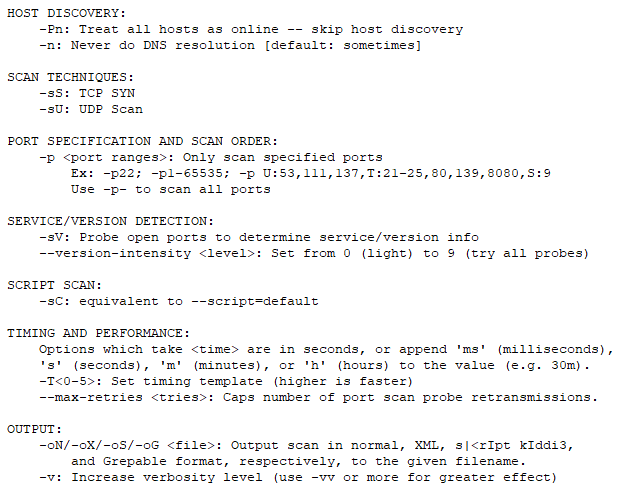
\includegraphics[scale=0.65]{images/nmap_Dokumentation} 
\caption{Auszug aus der Dokumentation des Programms nmap. Die hier dargestellten Optionen des Programmes beziehen sich auf die im Verlauf der Arbeit eingesetzten Optionen. Quelle: https://svn.nmap.org/nmap/docs/nmap.usage.txt (Abgerufen am 02.01.2020)}
\label{fig:nmap Dokumentation}
\end{center}
\end{figure}

Zur Prüfung der WLAN-Schnittstelle wurde auf die Programmsuite aircrack-ng zurückgegriffen. Es handelt sich hierbei um eine frei verfügbare Sammlung von Programmen zur Analyse der Sicherheit von Wi-Fi Netzwerken \cite{ThomasdOtreppedeBouvette.25.01.2020}. Zunächst wird das Programm airmon-ng eingesetzt, um die WLAN-Karte in den sogenannten Monitor-Modus zu versetzen:\\

\begin{lstlisting}[language=sh,caption={Kommando um die WLAN-Karte in den Monitormodus zu versetzen. Der Name der verwendeten Karte ist wlan0.}]
$ airmon-ng start wlan0
\end{lstlisting}


\noindent Daraufhin kann airodump-ng verwendet werden, um Informationen zu allen verfügbaren WLAN-Netzen bereitzustellen: \\

\begin{lstlisting}[language=sh,caption={Kommando um airodump-ng mit der soeben in den Monitormodus versetzen WLAN-Karte zu starten.}]
$ airodump-ng wlan0mon
\end{lstlisting}

\vfill \pagebreak

\noindent Vor allem die Spalte "`ENC“, welche für "`encryption“ steht, ist von Bedeutung. Sie zeigt an, dass das Gerät durch Wi-Fi Protected Access 2 (WPA2) geschützt ist. Dies unterstützt die Annahme, dass das Gerät WPA2 nach dem IEEE802.11i Standard bereitstellt. 

\begin{figure}[ht]
\begin{center}
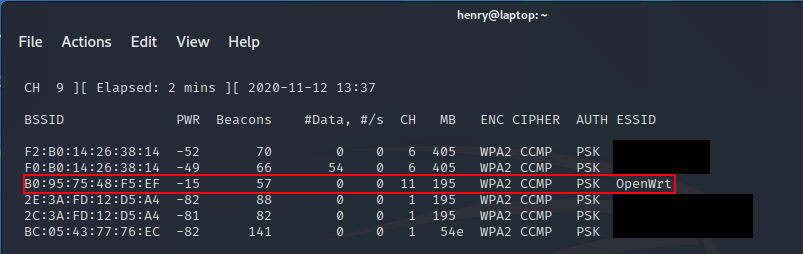
\includegraphics[scale=0.6]{images/airodump_output} 
\caption{Die Ausgabe des Programms airodump-ng. Man kann sehen, dass OpenWrt mit WPA2 CCMP verschlüsselt ist und ein Password (Spalte PSK) benötigt. }
\label{fig:Airodump-ng Ausgabe}
\end{center}
\end{figure}

\end{onehalfspace}


\subsubsection{Modul B - Public Network}
\begin{onehalfspace}
Die Teststrategie, welche für Modul B – Public Network eingesetzt wurde, ist nahe an der Vorgehensweise von Modul A – Private Network orientiert. Jedoch wird nun die IP des OpenWrt Geräts im Kontext des Subnetzes 192.168.178.0/24 verwendet (siehe Abbildung \ref{fig:Testumgebung TR}). So wird nicht die LAN-Schnittstelle des Gerätes angesprochen, sondern die WAN-Schnittstelle, also die öffentliche IP-Adresse des Gerätes ist.\\

\begin{lstlisting}[language=sh,caption={nmap Kommandos zum Scannen der WAN-Schnittstelle von OpenWrt. Das erste Kommando scannt TCP, das zweite UDP. Die angegebene IP-Adresse ist die des OpenWrt Routers.}]
$ # Fuer TCP:
$ nmap -sSCV -p- -Pn -oN <Dateiname.txt> 192.168.178.115
$ # Fuer UDP:
$ nmap -n -sUV --version-intensity 0 -p- --max-retries 1 -v -oN <Dateiname.txt> 192.168.178.115
\end{lstlisting}

\noindent Auch die VoIP Funktionalität kann effektiv mit nmap getestet werden. Zusätzlich zu einem vollständigen Scan des Geräts wurden auch die standardmäßig für VoIP verwendeten Ports 5060 und 5061 separat gescannt. \vfill \pagebreak

\begin{lstlisting}[language=sh,caption={Kommandos zum gezielten Scan der Ports 5060, 5061 mit nmap.}]
$ # TCP Port 5060, 5061 testen
$ nmap -sSCV -p 5060,5061 -Pn -oN <Dateiname.txt> 192.168.178.115
$ # UDP Port 5060, 5061 testen
$ nmap -n -sUV --version-intensity 0 -p 5060,5061 --max-retries 1 -v -oN <Dateiname.txt> 192.168.178.115
\end{lstlisting}

\noindent Jedoch sollte eine vollständige Prüfung aller Ports in jedem Falle durchgeführt werden, da diese Ports nicht zwingend genutzt werden müssen. 	

\end{onehalfspace}

\subsubsection{Modul C - Functionalities}
\begin{onehalfspace}
Das "`Test Requirement"{} TR.C.2 beschreibt die Anforderung, dass dem Endnutzer keinerlei Funktionalität verheimlicht werden darf. Dies ist eine durchaus schwierig zu prüfende Anforderung, welche erst zum Ende des Tests durchgeführt werden sollte. Im Falle von OpenWrt und dem somit vollständig verfügbaren Quellcode, sowie dem vollumfänglichen root Zugriff auf das Gerät per SSH ist dies vereinfacht, jedoch aufgrund des Funktionsumfangs immer noch eine Herausforderung. Es muss sich hier auf die Eindrücke und Erfahrungen des Testers zum Ende der Testphase verlassen werden. Darüber hinaus verweist die Technische Richtlinie ebenfalls auf eine Recherche in Foren und Blogs.
\end{onehalfspace}

\subsubsection{Modul D – Configuration and Information}
\begin{onehalfspace}
Für die meisten modernen Heimrouter ist die Konfiguration durch ein Web-Interface die benutzerfreundlichste Methode, so auch für OpenWrt. Die Sicherung der Datenintegrität und Vertraulichkeit auf dem Transportweg wird heutzutage durch HTTPS erreicht. Diese Transportwegverschlüsselung verhindert, dass eine böswillige dritte Partei die übertragenen Daten auslesen oder verändern kann (siehe Abschnitt \ref{Angriffe}. Es ist also naheliegend, die Anforderung an eine durch HTTPS gesicherte Verbindung zum Webserver in der Technischen Richtlinie zu finden. Zur Überprüfung des "`Test Requirement"{} TR.D.3 bietet sich ein Skript wie testssl.sh an, welches von Dr. Wetter IT-Consulting frei zur Verfügung gestellt wird \cite{D.Wetter.2020}. Dieses Skript zeigt detaillierte Informationen zu allen vom Webserver unterstützten Protokollversionen sowie Verschlüsselungsmethoden an. Des Weiteren kann auch ein Paketaufzeichnungs- und Analyse-Software wie Wireshark eingesetzt werden, um die unverschlüsselten Pakete zu betrachten. Wenn HTTPS aktiv ist, sollten keine unverschlüsselten Daten in den Paketen gefunden werden können. Es ist ebenfalls möglich, Informationen zu HTTPS und dem dazugehörigen Zertifikat in den meisten modernen Browsern in der Nähe der URL-Leiste zu finden. \newline\indent	
	Nichtsdestoweniger müssen auch andere Angriffsvektoren auf Heimrouter betrachtet bzw. getestet werden. So muss das Einloggen auf dem Gerät gegen Bruteforce Angriffe (vgl. Abschnitt \ref{bruteforce}) geschützt sein. Eine Schutzmaßnahme kann ein Fehlerzähler sein, welcher die fehlgeschlagenen Versuche protokolliert und das Aufschalten auf das Gerät nach einer gewissen Anzahl an Versuchen unterbindet oder verlangsamt. Ebenso könnte die Eingabe auf Muster geprüft werden, um automatische Login-Versuche zu erkennen. Die Prüfung dieses "`Test Requirements"{} wurde durch ein Skript in der Programmiersprache Python umgesetzt. Durch den Aufruf 	\\

\begin{lstlisting}[language=sh,caption={OpenWrt Webserver mit Python Skript auf Resistenz gegen Bruteforce Angriffe testen. (Das Programm ist auf dem Datenträger verfügbar) }]
$ python3 OpenWrt_Bruteforce_Check.py web 
\end{lstlisting}

\noindent wird der Web-Server getestet. Alternativ kann durch \\

\begin{lstlisting}[language=sh,caption={OpenWrt SSH-Server mit Python Skript auf Resistenz gegen Bruteforce Angriffe testen.}]
$ python3 OpenWrt_Bruteforce_Check.py ssh
\end{lstlisting}

\noindent der SSH Server getestet werden. Vor der Nutzung können der korrekte Benutzername, sowie das korrekte Password, die Anzahl der Versuche, die IP des Geräts, sowie der SSH-Port festgelegt werden. Für den Test des SSH-Servers wurden 100 Versuche eingestellt, wobei die Zeit für die Antwort des Servers gemessen wird. Das Python Modul "`SSHLibrary“ wird genutzt, um die Verbindungen mit dem SSH-Server zu handhaben. Zunächst wird geprüft, ob der spezifizierte Server erreichbar ist. Daraufhin werden die spezifizierten Login Versuche durchgeführt und die Zeit bis zur Antwort des Servers gemessen. Die Antwort des Servers bei falschen Daten ist der Abbruch der Session durch eine SSHLibrary Exception. Nachdem die Daten gesammelt wurden, wird eine lineare Regression auf den Daten durchgeführt, um einen Trend in den Antwortzeiten kenntlich zu machen. Wenn ein linearer Anstieg zu erkennen ist, dann werden die Versuche verlangsamt, wenn die Regressionslinie jedoch zur X-Achse parallel ist, so werden die Versuche in konstanter Zeit durchgeführt. Neben der grafischen Darstellung der Antwortzeiten, sowie der Regressionslinie, werden dem Nutzer der Mittelwert, der Median, der Regressionskoeffizient und der Standardfehler angezeigt. Nachdem die Analyse durchgeführt wurde, werden die korrekten Login Daten verwendet, um eine neue Verbindung herzustellen. Wenn das OpenWrt SSH-Banner korrekt angezeigt wird, lässt der SSH-Server trotz der vorherigen fehlgeschlagenen Versuche noch weitere zu, ohne erkennbare Entschleunigung. Der Test des Webservers wurde durch die POST Anfrage \vfill \pagebreak

\begin{lstlisting}[language=html]
http://192.168.1.1/cgibin/luci/admin/status?luci_username={USERNAME}
                                                          &luci_password={PASSWORD}
\end{lstlisting}


\noindent realisiert. Wenn ein falscher Benutzername, oder ein falsches Passwort verwendet wird, so antwortet der Webserver mit dem Statuscode 403. Nach der ersten Überprüfung der Verbindung wurden erneut 100 Versuche eingestellt. Dieser Wert wurde gewählt, um eine möglichst große Stichprobengröße zu erzielen und den unter Umständen implementierten Grenzwert für Login-Versuche zu überschreiten. Der weitere Ablauf der Analyse verläuft wie bereits beschrieben. Nach der Auswertung der Daten werden die korrekten Login-Daten an den Server geschickt. Ein einfacher regulärer Ausdruck überprüft, ob ein erfolgreicher Login möglich war, und es wird dem Benutzer anschließend angeboten, eine eingeloggte Session im \mbox Browser zu öffnen.	\\ \indent
	Zur Überprüfung der Anforderung TR.D.12 wird zunächst festgestellt, ob es einen Anti-CSRF Cookie (vgl. Abschnitt \ref{CSRF}) gibt. Zunächst kann der Speicher des Webbrowsers angezeigt werden, um zu prüfen, ob überhaupt ein Cookie eingesetzt wird. Daraufhin wird die Web-Proxy Funktionalität von Burp Suite genutzt, um den Ablauf des Logins und der Erstellung einer gültigen Session zu beobachten. Dabei handelt es sich um ein Programm, welches die Anfragen des Nutzers und des Servers entgegen nimmt und stellvertretend an den jeweils anderen vermittelt. Die Besonderheit bei Burp Suite ist dabei, dass die Anfragen zunächst abgefangen werden und der Inhalt für den Nutzer dargestellt wird. Auf diese Weise lässt sich die gesamte Kommunikation zwischen einem Client und einem Server beobachten (vgl. Abbildung \ref{fig:Proxy}). Alternativ zu Burp Suite kann auch der \glqq Zed Attack Proxy\grqq{} (ZAP) des \glqq Open Web Application Security Project\grqq{} (OWASP) eingesetzt werden \cite{ZAP.2020}. Alle nachfolgenden http-Methoden sollten nach Initialisierung des Cookies diesen als Sicherheitsmerkmal mit versenden. Der Quellcode von OpenWrt gibt darüber hinaus weiteren Aufschluss über die Implementierung der Anti-CSRF Tokens. Die Datei "`dispatcher.lua“ des LuCI Interfaces, welche die Erstellung und Validierung der \mbox Benutzer-Sitzungen handhabt, zeigt in diesem Falle eindeutig, dass es sich um Anti-CSRF Cookies handelt und dass diese durch den als sicher anerkannten Zufallszahlengenerator \mbox /dev/urandom generiert werden \cite{OpenWrtLuci.2020, PatrickLacharme.2012}. Abschließend wurde ein einfaches Python Skript verwendet, welches 100 gültige Sitzungen am Web Server des OpenWrt Routers anmeldet und mittels eines Regulären-Ausdruckes den Wert des Cookies ausließt. Dazu wird das Request Modul von Python verwendet, sowie die POST-Anfrage, welche bereits für das Bruteforce-Skript verwendet wurde. Abschließend wird geprüft, ob die 100 verschiedenen Sitzungen einzigartige Session-IDs und Anti-CSRF Token besitzen.	


\begin{figure}[h]
\begin{center}
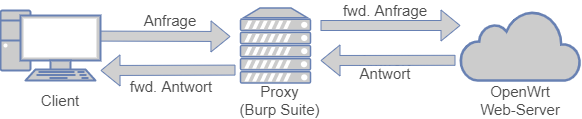
\includegraphics[scale=0.5]{images/proxy} 
\caption{Vereinfachte Darstellung eines MITM-Proxies wie Burp Suite.}
\label{fig:Proxy}
\end{center}
\end{figure}	

\end{onehalfspace}


\subsubsection{Modul E – Firmware Updates}
\begin{onehalfspace}
Modul E der Technischen Richtlinie prüft die Firmware Update Funktion des Geräts. Hier ist vor allem der Mechanismus der Firmware-Validierung von Interesse. Nach Angaben der Entwickler werden einige Firmware Dateien signiert. OpenWrt liefert standardmäßig ein Kommandozeilenprogramm, mit dem Signaturen und Metadaten aus den Firmwareabbildern extrahiert werden können. Der Aufruf \\	 

\begin{lstlisting}[language=sh,caption={Nutzung des in OpenWrt integrierten Programmes "`fwtool“ zur Extraktion von Signaturen aus OpenWrt Firmware-Abbildern}]
$ fwtool -s - <Dateiname.bin> 
\end{lstlisting}

\noindent zeigt die Signatur an, wenn diese vorhanden ist. Ebenso muss ermessen werden, wie lange der Hersteller benötigt, um Sicherheitslücken zu beheben. Die sogenannten "`Git Hashes“, genaue Identifizierungsmerkmale eines git commits, sind hier förderlich, da sie einen genauen Zeitstempel tragen. Des Weiteren ist der entsprechende git commit, welcher eine Sicherheitslücke behebt, in den Sicherheitsnotizen auf der OpenWrt Website spezifiziert, sodass das Erstellen einer Zeitleiste mit Sicherheitsvorfällen und deren Beheben einfach realisierbar ist. 	 
\end{onehalfspace}



\subsubsection{Modul G – Domain Name System (DNS)}
\begin{onehalfspace}
Zur weiteren Einschränkung der Angriffsoberfläche wird in Modul G die Implementierung des DNS-Dienstes des DUT geprüft. Ein möglicher Angriff auf DNS-Dienste ist eine sogenannte DNS Rebinding Attacke (vgl. Abschnitt \ref{rebinding}). Die Überprüfung der Anforderung TR.G.2 basiert auf der Untersuchung der verwendeten Methoden zur Mitigation von DNS Rebinding Attacken und einem funktionalen Test dieser Umsetzung. Da OpenWrt DNS-Dienste mittels dnsmasq anbietet, muss geprüft werden, ob die Option "`--stop-dns-rebind“ aktiviert ist. Dies ist sowohl über die Kommandozeile als auch über das LuCI Web-Frontend möglich. Ein funktionaler Test dieser Sicherheitsmaßnahme kann mittels des Singularity of Origin Web-Toolkits der NCC Group getestet werden \cite{GeraldDoussot.2019}. Als Target Host wird dabei die IP-Adresse des OpenWrt Routers spezifiziert. Des Weiteren wurde das Intervall auf zwei reduziert und die Option "`Flood DNS Cache“ aktiviert. Diese Option konnte genutzt werden, da der Test mit einem Chromium basierten Browser durchgeführt wurde. Das Web-Tool spezifiziert, dass diese Option erfolgreich im Chrome-Browser getestet wurde (vgl. Abbildung \ref{fig:Singularity Web Interface}). Es bietet sich ebenfalls an verschiedene "`Attack Payloads“ und Strategien zu testen. \\

\begin{figure}[ht]
\begin{center}
\includegraphics[scale=0.3]{images/Singularity_web} 
\caption{Das Singularity of Origin Web-Interface. Die Webseite wird von der NCC Group bereitgestellt, um verschiedene Arten von DNS Rebinding Angriffen zu testen. In diesem Kontext wurde es genutzt, um zu prüfen, ob OpenWrt diese Angriffe erfolgreich abwehrt bzw. erkennt. \protect\url{http://rebind.it:8080/manager.html}}
\label{fig:Singularity Web Interface}
\end{center}
\end{figure}



\indent Eine ebenso relevante Sicherheitsfunktion von DNS-Diensten ist die sogenannte "`Source Port Randomization“ und "`Transaction ID Randomization“, also die zufällige Wahl eines Quell-Ports, sowie einer Transaktions-ID für eine DNS-Anfrage. Diese Werte, welche vom DNS-Client generiert werden, dienen als Synchronisationsmethode zwischen dem DNS-Server und Client. Wenn der Quell-Port und die Transaktionsidentifikationsnummer von einem Angreifer berechnet oder geraten werden können, dann kann ein Angreifer diese nutzen, um dem Opfer manipulierte DNS-Antworten zu senden. Der DNS-Client würde diese aber als korrekt akzeptieren und eine potenziell schädliche Verbindung zu einem dritten Server aufbauen \cite{Microsoft.2008}. Für einen funktionalen Test werden zunächst mithilfe des Python Skriptes send\_dns\_requests.py eine große Anzahl verschiedene DNS-Anfragen generiert. Dazu wird eine Liste mit 1000 häufig besuchten Webseiten genutzt \cite{BenSooter.15.03.2016}. Dies bietet sich an, da so sichergestellt wird, dass diese Webseiten verfügbar sind und in einer geringen Zeit antworten. Ebenso erfüllt diese Anzahl an Anfragen die minimale Stichprobengröße ($n$) für $\rho = 0.5$ (Stichprobenfehler $e = 0.03$ / Signifikanzniveau $\alpha = 0.05$) \cite[p.~13]{Gabler2016}. Während die DNS-Anfragen gestellt werden wird ein Mitschnitt aller Netzwerkpakete durch das Programm Wireshark gemacht. Die so erstellte Datei wird in einem weiteren Schritt analysiert. Dazu liest das Python-Skript "`analyze\_pcap.py“ diese ein und selektiert im ersten Schritt alle DNS-Pakete, welche vom OpenWrt Router gesendet wurden. Daraufhin werden der DNS-Quell-Port sowie die Transaktions-ID aus diesen Paketen ausgelesen. Im letzten Schritt werden die Anzahl der DNS Anfragen, die Anzahl der einzigartigen Ports und Transaktions-IDs, die jeweiligen minimalen und maximalen Werte, die Standardabweichung und die häufigsten Werte angezeigt. Des Weiteren wird ein Kolmogorow-Smirnow-Test durchgeführt, um zu prüfen, ob die Verteilung der Daten mit einer Gleichverteilung übereinstimmt \cite{Frank1951}. Schlussendlich werden noch jeweils zwei Grafiken generiert, welche die Daten in einem Säulendiagramm und einen Streudiagramm darstellen. Auf diese Art kann visuell prüfen, ob Muster in den Darstellungen zu erkennen sind. \\

\vspace{1cm}

\lstinputlisting[language={},caption={Ergebnisse der DNS Port und DNS Transaktions-Identifikationsnummern Analyse. Der Kolmogorow-Smirnow Test zeigt, dass die Daten annähernd gleichverteilt sind.}]{images/DNS_port_and_id_distribution_analytics.txt}

\vfill \pagebreak

\begin{figure}[ht]
\begin{center}
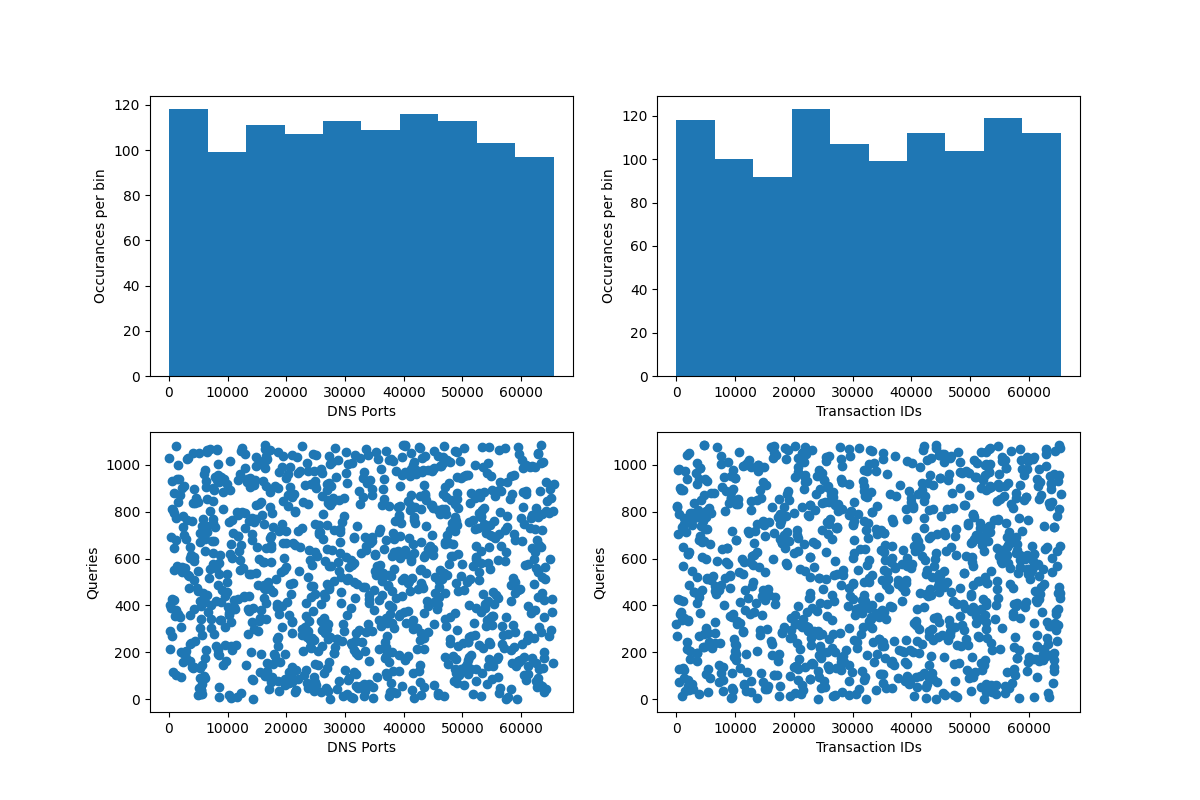
\includegraphics[scale=0.5]{images/DNS_port_and_id_distribution_graph.png} 
\caption{Darstellung der Ergebnisse als Säulendiagramm und als Streudiagramm. Die X-Achse beschreibt die Source-Ports bzw. die Transaktions-ID. Aus der Y-Achse der Säulendiagramme sind ist die Häufigkeit pro Sammelbehälter dargestellt. Die Y-Achse der Streudiagramme zeigt die Anzahl der Anfragen. Man kann sehen, dass die volle Spannbreite von 0 bis 65535 ausgenutzt wird. Da kein Muster in den Streudiagrammen erkennbar ist und die Säulendiagramme eine Gleichverteilung andeuten, kann angenommen werden, dass zufällige Source-Ports und Transaktions-IDs gewählt wurden. }
\label{fig:DNS Randomization}
\end{center}
\end{figure}

\end{onehalfspace}



\subsubsection{Modul I – Factory Reset}
\begin{onehalfspace}
Das Testen der Zurücksetzfunktion des OpenWrt Routers fällt aufgrund des uneingeschränkten Systemzugriffs einfach. Es können verschiedene Methoden eingesetzt werden. Zunächst sollte eine Leitlinie (Baseline) erstellt werden. Dazu dient ein Konfigurationsbackup, welches direkt nach dem ersten Einschalten des Geräts erstellt wurde. Dieses wird anschließend mittels des Kommandozeilenprogramms "`diff“ mit einem Backup verglichen, welches nach der Nutzung des Routers und einem anschließenden Zurücksetzen des Geräts erstellt wurde. Alternativ kann das ebenfalls auf OpenWrt zur Verfügung stehende Kommandozeilenprogramm \glqq md5sum\grqq{} verwendet werden, um MD5 Hash-Werte aller lesbarer Dateien auf dem System zu generieren und diese zu exportieren. Diese sollten nach dem Zurücksetzen des Geräts wieder übereinstimmen. Die Erstellung von CRC-Prüfsummen mit dem \glqq cksum\grqq{} Befehl kann unter Umständen schneller sein, als MD5 Hash-Werte. Es bietet sich also an diese Prüfsummen auf leistungsschwachen Geräten zu verwenden. Da die MD5 Hash-Werte und CRC Summen lediglich genutzt werden sollen, um zu prüfen, ob Einstellungen zurückgesetzt wurden, sind an dieser Stelle keine kryptografisch sicheren Hash-Werte wie SHA256 nötig. Die Wahrscheinlichkeit für zufällige Kollisionen bei MD5 ist sehr gering \cite{Rivest.1992}. Darüber hinaus werden diese Prüfsummen bzw. Hash-Werte ausschließlich in einem lokalen System generiert und verwendet. 
\end{onehalfspace}

\subsection{Nicht anwendbare Test Prozeduren}
\begin{onehalfspace}
Ebenso wie die Natur des OpenWrt Projektes ein einfaches Testen vieler "`Test \mbox Requirements"{} ermöglicht, so werden einige Aspekte der Firmware anders gehandhabt als bei handelsüblichen Heimroutern. So sucht man vergeblich nach einem initial verfügbaren WLAN-Netz, nachdem der Router gestartet und eingerichtet wurde. Ebenso sind viele Funktionen, die ein Nutzer vielleicht von anderen Geräten gewöhnt ist, nur als zusätzliches Software-Paket verfügbar, oder durch aufwendige Konfiguration. Beispiele sind Wi-Fi Protected Setup, ein Community WLAN, Fernwartung, automatische Firmware-Updates oder Meldungen zu neuen Firmware-Updates, Voice over IP und Virtual Private Network Funktionen. 
\end{onehalfspace}

\section[Statische Code-Analyse mit FACT]{Statische Code-Analyse einiger quelloffenen Router Firmware Alternativen mittels FACT}
\label{statische CodeA}
\begin{onehalfspace}
Neben der Methodik der Technischen Richtlinie des BSI gibt es noch viele weitere Arten, um Aspekte einer Software zu evaluieren. Die Sicherheit einer betrachteten Software, in diesem Fall OpenWrt, lässt sich unter anderem durch sogenannte statische Tests abschätzen (siehe Abschnitt \ref{Softwaretests}). Es wird sich für die Durchführung einer statischen Code-Analyse von Router-Firmware an der Methodik des "`Home Router Security Reports 2020“ des Fraunhofer-Institut für Kommunikation, Informationsverarbeitung und Ergonomie (FKIE) orientiert \cite{PeterWeidenbachJohannesvomDorp.2020}. In dieser Veröffentlichung des FKIE wurden 127 verschiedene, aktuelle Firmware-Abbilder von sieben Herstellern automatisch durch das ebenfalls vom FKIE entwickelte \glqq Firmware Analysis and Comparison Tool\grqq{} (vgl. Abschnitt \ref{FACT}) analysiert und ausgewertet.
\end{onehalfspace}


\subsection{Installation und Testumgebung}
\begin{onehalfspace}
FACT, welches vom FKIE kostenfrei zur Verfügung gestellt wird, wurde lokal auf einem Desktop Computer installiert. Es handelt sich hierbei um ein System mit 6 physischen und 6 virtuellen Prozessorkernen, welche jeweils auf einer Taktfrequenz von 4.2GHz betrieben werden, sowie 16GB RAM. Ebenfalls stehen dem System 256GB persistenter Speicher zur Verfügung. Da die Installation auf Ubuntu 16.04, 18.04, 20.04 (stable) empfohlen wird, wurde Ubuntu 20.04 als aktuellster Vertreter des Ubuntu-Betriebssystems ausgewählt \cite{FraunhoferFKIE.2020b}. Die zum Zeitpunkt der Arbeit aktuelle Version von FACT, FACT\_core v3.1.1, wurde mittels der bereitgestellten Anleitung installiert (siehe \ref{installation}) \cite{FraunhoferFKIE.2020}. \\


\begin{lstlisting}[language=sh,label={installation}, caption={Installationsschritte für das \glqq Firmware Analysis and Comparison Tool\grqq{} des FKIE. Diese Schritte Updaten die installierten Pakete, downloadet das Git Repository und führt alle nötigen Schritte zur Installation aus. Zuletzt wird das Programm gestartet.}]
$ sudo apt update && sudo apt upgrade && sudo apt install git
$ git clone https://github.com/fkie-cad/FACT_core.git ~/FACT_core
$ ~/FACT_core/src/install/pre_install.sh && sudo mkdir /media/data && sudo chown -R USER /media/data
$ sudo reboot
$ ~/FACT_core/src/install.py
$ ~/FACT_core/start_all_installed_fact_components

\end{lstlisting}

\noindent Da das System den minimalen Software Anforderungen von FACT entspricht ist die Installation und Nutzung des Programms prinzipiell möglich, jedoch empfiehlt sich ein System mit mehr RAM, da dies die Performanz der Analyse erhöht. Ebenfalls kam es bei dem eingesetzten System vermehrt dazu, dass kein RAM mehr zur Verfügung stand und der Rechner während der Analyse aufgrund der Auslastung nicht anderweitig genutzt werden konnte. Der Einsatz eines separaten Test Computers oder eines Virtuellen Privaten Servers (VPS) ist zu empfehlen. \\

\begin{figure}[ht]
\begin{center}
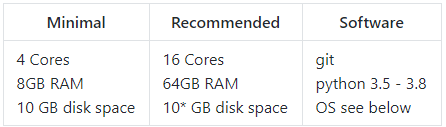
\includegraphics[scale=0.7]{images/FACT_system_requirements} 
\caption{Minimale und empfohlene Systemvorraumsetzungen für FACT. Die Grafik stellt auch die benötigte Software dar. \cite{PeterWeidenbachJohannesvomDorp.2020} }
\label{fig:FACT System Requirements}
\end{center}
\end{figure}


\end{onehalfspace}


\subsection{Erstellung des Firmware-Corpus}
\begin{onehalfspace}
Der zu testende Firmware-Corpus besteht aus sieben verschiedenen, quelloffenen Router-Firmwares. Neben dem für die Technische Richtlinie verwendeten Abbild von OpenWrt Version 19.7.04, wurden noch sechs weitere Alternativen gewählt, von denen fünf spezifisch für das gewählte TP-Link Model Archer C7 v5 kompiliert sind. Zu der betrachteten \mbox Firmware gehören DD-WRT, Gargoyle Router Management, Gluon, LibreCMC, AdvancedTomato, sowie Version 19.7.05 von OpenWrt. Einzig AdvancedTomato bietet keine Version für den getesteten Router an, weshalb auf eine Version für einen NETGEAR WNDR3700v3 Dual-Gigabit-WLAN-Router zurückgegriffen wurde, da dieser Router ebenfalls eine MIPS Architektur nutzt und im Leistungsumfang vergleichbar ist. 	\\ 
\indent Die aufgelistete Firmware wurde gewählt, da sie in Funktion und Umfang OpenWrt ähnlich sind und die Projekte, denen sie entstammt, ebenfalls mehrere Heimrouter mit einer Codebasis unterstützen. Es wurden keine Firmware-Alternativen gewählt, die auf Desktop Computern oder Servern installiert werden, da diese aufgrund der zur Verfügung stehenden Rechenkapazitäten im Leistungsumfang nicht vergleichbar sind. Das analysierte Korpus wurde am 21.12.2020 erstellt. Es wurde für jede analysierte Firmware die aktuellste Version für den TP-Link AC1750-Dualband-Gigabit-WLAN-Router genutzt, mit Ausnahme des Abbildes von OpenWrt Version 19.07.4 und der Tomato Firmware. Version 19.07.4 wurde getestet, da es sich um die mittels der Technischen Richtlinie geprüfte Version handelt. \\ 

\begin{table}[ht]
\begin{center}
\def\arraystretch{1.4}
%\resizebox{\textwidth}{!}{%
\begin{tabular}{lll}

\textbf{Projekt} & \textbf{Geeignetes Produkt} & \textbf{Firmware Version} \\ 
\hline 
AdvancedTomato & NETGEAR WNDR3700v3 & 3.4-138 \\ 

DD-WRT & TP-Link Archer C7 v5 & 12-18-2020-r45036 \\ 

Freifunk Gluon & TP-Link Archer C7 v5 & V2-v2020.2.1 \\ 

Gargoyle Router Management & TP-Link Archer C7 v5 & 1.12.0 (stable) \\ 

LibreCMC & TP-Link Archer C7 v2 & v1.5.3:2020-10-02 \\ 

OpenWrt & TP-Link Archer C7 v5 & 19.07.4 \\ 

OpenWrt & TP-Link Archer C7 v5 & 19.07.5 \\ 

\end{tabular}%
\end{center}
%}
\caption{Übersicht über die für die Analyse ausgewählte Firmware. Dargestellt ist jeweils der Name des Projektes, das Produkt für das die Firmware geeignet ist und die ausgewählt Version der Firmware (vollständige Tabelle: Anhang \ref{tab:Untersuchte Firmware})}
\label{tab:Untersuchte Firmware}
\end{table}

\end{onehalfspace}


\subsection{Durchgeführte Tests und Metriken}
\begin{onehalfspace}
Um einen Vergleich mit den Ergebnissen des \glqq Home Router Security Reports 2020\grqq{} des FKIE zu ermöglichen, wurden die gleichen Aspekte auch bei der quelloffenen Firmware analysiert. Es wurden die folgenden sicherheitsrelevanten Aspekte betrachtet:

\begin{itemize}
\item Wann wurde das letzte Update für das Gerät veröffentlicht?
\item Welches Betriebssystem wird verwendet und wie viele kritische Schwachstellen sind für dieses bekannt?
\item Welche vorbeugenden Maßnahmen gegen Exploits werden eingesetzt und wie häufig sind diese aktiviert.
\item Ist privates kryptografisches Schlüsselmaterial enthalten?
\item Können hartkodierte Login-Daten und bekannte Passwörter in dem Firmware-Abbild gefunden werden?
\end{itemize}

\noindent Die einzelnen Komponenten des "`Firmware Analysis and Comparison Tools“ werden mittels des Befehls \\

\begin{lstlisting}[language=sh,caption={Befehl zum starten alle Komponenten von FACT}]
$ ~/FACT_core/start_all_installed_fact_components
\end{lstlisting}

\noindent gestartet. Nachdem der lokale Server gestartet ist, werden die Firmware-Abbilder einzeln über die Upload-Funktion hochgeladen. Die folgenden Analyse-Methoden wurden gewählt:
\end{onehalfspace}

\begin{itemize}
\item CPU Architecture
\item Crypto Material
\item CVE Lookup
\item CWE Checker
\item Exploit Mitigations
\item Known Vulnerabilities
\item Software Components
\item Source Code Analysis
\item Users and Passwords
\end{itemize}
\begin{onehalfspace}
\noindent Die Ergebnisse der automatischen Analyse werden anschließend durch die REST API von FACT ausgelesen und als Grafiken dargestellt, sodass eine direkte Gegenüberstellung der Ergebnisse des FKIE mit den erhobenen Daten möglich ist. 

\end{onehalfspace}




%############################################################################################
% Ergebnisse




\chapter{Ergebnisse}
\section{Ergebnisse der Technischen Richtlinie}
\label{erg_tr}

\begin{onehalfspace}
Von 101 "`Test Requirements"{} konnte der TP-Link Router in 69 getestet werden. Bei den 32 nicht getesteten Fällen handelt es sich in den meisten Instanzen um Funktionalität, welche von dem Gerät ohne weitere Software-Pakete nicht unterstützt wird. So wurden die “Module K – Remote Configuration”, “Modul L – Voice over IP” und “Modul M – Virtual Private Network” vollkommen vom Testvorgang ausgeschlossen. Ebenso wurden "`Test Requirements"{} nicht geprüft, welche mit den bereits genannten Modulen Gemeinsamkeiten haben. Darüber hinaus fielen Testfälle bezüglich der standardmäßig gesetzten Passwörter und Login-Daten ebenso weg wie solche, die Community-Funktionen testen. Die 69 getesteten Anforderungen umfassten 109 Test Prozeduren, von denen wiederum 9 als ergebnislos gewertet wurden. Grafik \ref{fig:Erfolgsrate OpenWrt} zeigt, dass 72\% (78 Test Prozeduren) als bestanden gelten, während 22\% (24 Test Prozeduren) als durchgefallen gewertet wurden. Nachfolgend werden zunächst die bestandenen Testfälle betrachtet und anschließend Änderungsvorschläge für nicht bestandene Testfälle beschrieben (siehe Unterkapitel \ref{anderungen}). \\ 

\begin{figure}[ht]
\begin{center}
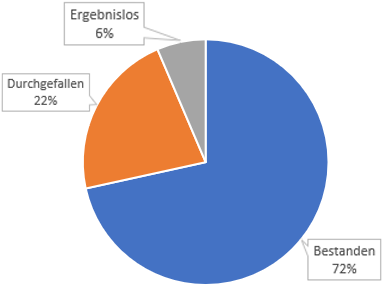
\includegraphics[scale=0.65]{images/tr_stat2} 
\caption{Darstellung der bestandenen, durchgefallenen und nicht anwendbaren Testfälle der Technischen Richtlinie bei der Untersuchung von OpenWrt. Es wurden insgesamt 69 \glqq Test Procedures\grqq{} durchgeführt. Die Testfälle werden in der Grafik ohne Gewichtung dargestellt.}
\label{fig:Erfolgsrate OpenWrt}
\end{center}
\end{figure}


\begin{footnotesize}
\begin{table}[t]
\centering

\begin{tabular}{lll}
\textbf{Kondition}                    & \textbf{Status} & \textbf{Anzahl} \\
\hline
MUST - Kriterium             & Passed & 49     \\
SHOULD  - Kriterium          & Passed & 13     \\
MUST - Kriterium             & Failed & 12     \\
SHOULD  - Kriterium          & Failed & 8      \\
MUST NOT - Kriterium         & Passed & 7      \\
MUST   - Kriterium           & Inc.   & 4      \\
MUST NOT - Kriterium         & Failed & 1      \\
MUST   NOT - Kriterium       & Inc.   & 1      \\
MAY - Kriterium              & Passed & 1      \\
MAY   - Kriterium            & Failed & 1      \\
MUST - Kriterium / MAY       & Passed & 1      \\
MUST   - Kriterium / MAY     & Inc.   & 1      \\
RECOMMENDED  -    Kriterium  & Failed & 1      \\
SHOULD  - Kriterium          & Inc.   & 0      \\
SHOULD NOT  -    Kriterium   & Passed & 0      \\
SHOULD   NOT  -    Kriterium & Failed & 0      \\
SHOULD NOT  -    Kriterium   & Inc.   & 0      \\
MAY   - Kriterium            & Inc.   & 0      \\
MUST - Kriterium / Should    & Passed & 0      \\
MUST   - Kriterium / Should  & Failed & 0      \\
MUST - Kriterium / Should    & Inc.   & 0      \\
MUST   - Kriterium / MAY     & Failed & 0      \\
RECOMMENDED  -    Kriterium  & Passed & 0     
\end{tabular}
\caption{Darstellung der Anzahl an Testfällen pro Kondition und Status. Die Tabelle wird wie folgt gelesen: 49 Testfälle, welche mit \glqq MUST\grqq{} gekennzeichnet sind, wurden bestanden.}
\end{table}
\end{footnotesize}

	Die Durchführung der Technischen Richtlinie an dem mit OpenWrt betriebenen Gerät zeigte, dass OpenWrt die eigenen Ansprüche an Speicherverbrauch und Funktionalität einhalten kann. Das Gerät liefert Kernfunktionen eines Routers und legt dabei besonderes Augenmerk auf die Reduzierung der angebotenen Dienste auf ein Minimum. Die wiederholten Port-Scans mit nmap zeigten, dass lediglich der Webserver, SSH und der DNS/DHCP Dienst über TCP und UDP betrieben werden (siehe Listing \ref{init}, \ref{initUDP}) \\

\lstinputlisting[language={},label={init}, caption={Ergebnisse des OpenWrt nmap Scans für alle \textbf{TCP}-Ports des \textbf{LAN}-Interfaces.}]{images/nmap_openwrt_initalised_tcp.txt}

\vspace{0.6cm}

\lstinputlisting[language={}, label={initUDP},caption={Ergebnisse des OpenWrt nmap Scans für alle \textbf{UDP}-Ports des \textbf{LAN}-Interfaces.}]{images/nmap_openwrt_initalised_udp.txt}

\noindent Des Weiteren wurden an keiner Stelle Defizite bezüglich der Testkriterien in der Dokumentation der Software gefunden. Alle in der Technischen Richtlinie geforderten Informationen der Dokumentation konnten ermittelt werden. Neben diesen Ergebnissen sind der vollständig quelloffene Code des Betriebssystems und der vollständige root Zugriff auf das Gerät deutliche Indikatoren dafür, dass dem Nutzer keine Funktionen vorenthalten werden (TR.C.2). Durch die Reduzierung auf die wesentlichen Funktionen eines Routers verringert OpenWrt deutlich die Angriffsoberfläche und spielt somit den Zielen der TR-03148 zu. Die Ergebnisse in "`Module B – Private Networks“ unterstützen diese Aussage. Der OpenWrt Router stellt keinen Dienst auf der WAN-Schnittstelle zur Verfügung. \\

\lstinputlisting[language={},caption={Ergebnisse des OpenWrt nmap Scans für alle \textbf{TCP}-Ports des \textbf{WAN}-Interfaces.}]{images/nmap_wan_all_ports_tcp.txt}

\vspace{0.5cm}

\lstinputlisting[language={},caption={Ergebnisse des OpenWrt nmap Scans für alle \textbf{UDP}-Ports des \textbf{WAN}-Interfaces.}]{images/nmap_wan_all_ports_udp.txt}

So wurde auch das VoIP-Protokoll (vgl. Abschnitt \ref{Router}) nicht in der Standardinstallation mitgeliefert, da dieses für die Funktionalität als Router nicht relevant ist. Ebenfalls konnten die Tests nachweisen, dass OpenWrt international angesehene Standards wie IEEE802.11i erfolgreich inkorporiert. 	\\ \indent
 	OpenWrt besteht auch einige weitere Testfälle aufgrund der umfänglichen Informationen und Logs, welche das System für den Nutzer bereitstellt. Das Gerät führt umfassende System- und Kernel-Log Dateien ebenso wie Informationen über verbundene Geräte, aktive und bereitstehende Dienste, Firewall-Funktionen und das System selbst. Die Log-Dateien können über das \glqq Logread\grqq -Programm abgerufen werden, stehen aber nicht als Datei zur Verfügung \cite{OpenWrtWebsiteLogread}. Auch werden relevante Informationen wie End-of-Support und Mitteilungen zu Sicherheitslücken klar strukturiert auf der Webseite der Entwickler veröffentlicht. Die Veröffentlichung von Updates, welche Sicherheitslücken beheben, erfolgt dabei stets in wenigen Tagen oder Wochen. Vor allem Module F bis I, welche sich mit Firewall, DNS, DHCP und dem Zurücksetzen des Gerätes beschäftigen, wurden von OpenWrt vollständig bestanden. Dies ist auf die ebenso quelloffenen Komponenten zurückzuführen, welche schon \vfill \pagebreak \noindent seit vielen Jahren weiterentwickelt werden und in einigen Bereichen weit verbreitet sind. So nutzt OpenWrt iptables als Firewall und dnsmasq für DNS und DHCP Funktionalität. \\ 


\begin{figure}[ht]
\begin{center}
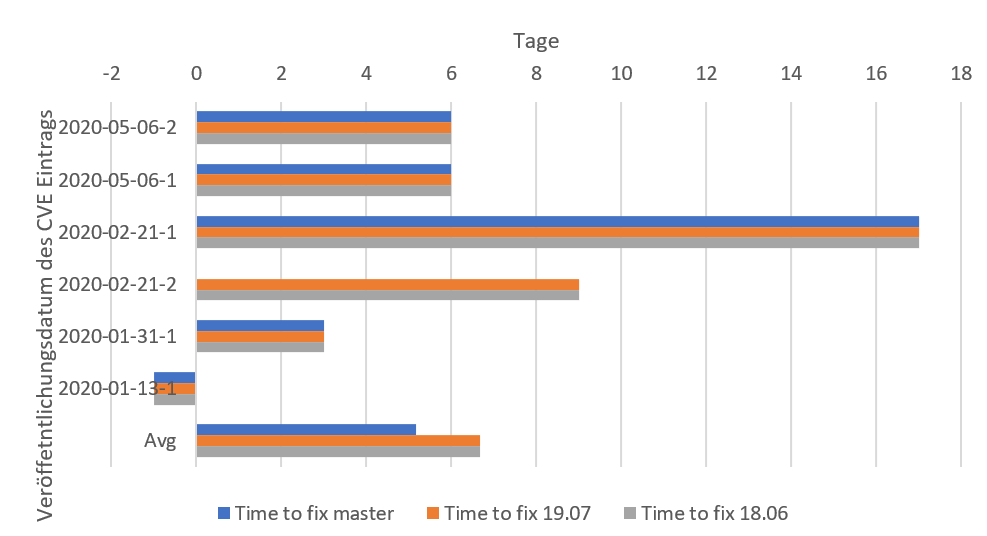
\includegraphics[scale=0.6]{images/days_to_fix_cve} 
\caption{Benötigte Zeit zur Implementierung und Veröffentlichung von Sicherheitsupdates für OpenWrt im Jahr 2020. Basiert auf dem Veröffentlichungsdatum des CVE-Eintrags und dem Datum des git commits, welcher im Sicherheitshinweis spezifiziert ist.}
\label{fig:Time to fix CVE}
\end{center}
\end{figure}	


 
\indent Einige Defizite bzw. gemischte Ergebnisse liefern die Testfälle des WLAN-Gästenetzes. Da OpenWrt keine klassische Funktionalität liefert, welche automatisch ein WLAN-Netz für Gäste bereitstellt, wurde hier auf die Anleitung in der Dokumentation zurückgegriffen, die ein ähnliches Ergebnis erzielen soll, jedoch dem Nutzer alle Freiheiten lässt, Änderungen zu machen. So ist es kein Garant, dass das Gäste-Netz Nutzer tatsächlich separiert oder, dass ein Nutzer nicht von dort aus auf die Konfiguration des Gerätes zugreifen kann. Die genaue Dokumentation der Ergebnisse kann auch im Ordner \glqq Results\grqq{} $\rightarrow$ TR.X $\rightarrow$ TP.X.Y abgerufen werden. 


\end{onehalfspace}

\section{Notwendige Änderungen zum Bestehen der Technischen Richtlinie}
\label{anderungen}
\begin{onehalfspace}
Wie bereits im vorherigen Kapitel festgehalten, benötigt OpenWrt nur einige Änderungen, um die Technische Richtlinie 03148 vollumfänglich zu bestehen. Es wird vor allem Wert auf die mit "`MUST“ gekennzeichneten Testfälle gelegt. Für Testfälle, die mit "`SHOULD“ gekennzeichnet sind wird nachfolgend eine Änderung vorgeschlagen, wenn es sich hierbei um eine simple Anpassung handelt. Darüber hinaus wurde die Funktionalität des Gäste-WLAN nicht weiter betrachtet, da dieses vom Nutzer vollständig konfiguriert werden muss. OpenWrt bietet keine Möglichkeit ein Gäste-Netzwerk mit einer einzigen Option zu aktivieren. Die vollständige Implementierung einer solchen Funktionalität müsste in Betracht gezogen werden.	\\ \indent
 	Es sind nur einige Änderungen von Nöten, um Modul A vollständig zu bestehen. Der 4. Test des Testfalls TR.A.9 (TP.A.9.4) schlägt fehl, da die Verschlüsselung von WLAN-Netzwerken standardmäßig ausgeschaltet ist. Im initialen Zustand ist die gesamte WLAN-Funktionalität von OpenWrt abgeschaltet. Sie muss zunächst vom Benutzer selbst in den Einstellungen, entweder über das Web-Interface oder SSH, eingeschaltet werden. In der Konfigurationsübersicht des jeweiligen WLAN-Netzes ist das Passwort jedoch erst in einem zweiten Reiter untergebracht. Dort ist standardmäßig "`No Encryption (open network)“ angewählt. Diese verzweigte Aufteilung kann dazu führen, dass unerfahrene Nutzer lediglich die ESSID anpassen und daraufhin den Speichern-Button betätigen. Auf diese Weise würde das Netzwerk ohne Passwort initialisiert. Das Verschieben des Passwortfeldes, sowie der Auswahl der Verschlüsselung in den ersten (initialen) Reiter der Übersicht, könnte diesem Problem entgegenwirken. Ebenso könnte die initiale Konfiguration der WLAN-Netzwerkes statt "`No Encryption“ stattdessen "`WPA2-PSK“ ausgewählt haben. So könnte der Nutzer die Konfiguration nicht speichern ohne ein Passwort einzufüllen. Wenn WPA2 ausgewählt ist, erscheint bei einem unzureichenden Passwort eine Fehlermeldung und die Konfiguration wird nicht gespeichert. Auf diese Weise kann dennoch gezielt ein Netzwerk ohne Passwort erstellt werden, wenn der Nutzer bewusst auf diese Option umgeschaltet hat. Eine noch stärkere Verschlüsselung bietet WPA3. Auf Geräten mit genügend Speicher könnten OpenWrt standardmäßig mit dem zusätzlichen Paket \glqq wpad-openssl\grqq{} ausgestattet werden. Auf diese Weise könnte statt WPA3 anstelle von WPA2 eingestellt werden (siehe Abbildung \ref{fig:Mockup}). Der Nutzer könnte ebenfalls von einem Mechanismus unterstützt werden, welcher die Stärke des WLAN-Passwortes darstellt. Ein ähnlicher Mechanismus wird bereits bei der Prüfung des Geräte-Passwortes eingesetzt und könnte auch im Umfeld des PSK dem Nutzer zusätzliche Hilfestellung bei der Wahl eines Passwortes geben. Dabei sollte der bestehende Mechanismus zur Evaluation des Passwortes allerdings angepasst werden, sodass die Vorgaben der Technischen Richtlinie eingehalten werden. \vfill \pagebreak

\begin{figure}[ht]
\begin{center}
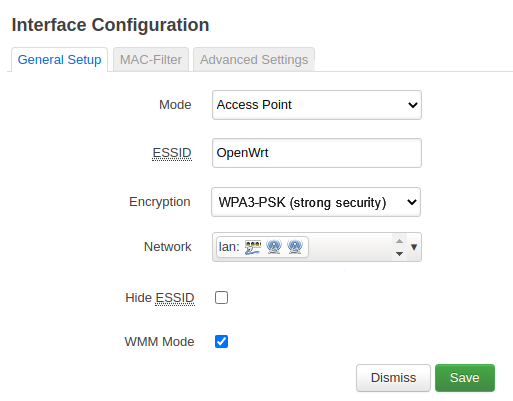
\includegraphics[scale=0.5]{images/mockup} 
\caption{Mockup der vorgeschlagenen Änderungen des WLAN-Konfigurationsmenüs von OpenWrt.}
\label{fig:Mockup}
\end{center}
\end{figure}	 	
 	
\indent Ein weiterer Test, welcher während der Durchführung der Technischen Richtlinie scheiterte, ist TR.D.2. Dieser beschreibt, dass der Zugang zur Konfiguration des Gerätes mindestens durch ein Passwort geschützt sein muss, wenn das Gerät sich im initialen oder kundenspezifischen Zustand befindet. Aufgrund der Natur vom OpenWrt als Alternatives Router-Betriebssystem, welches erst nach Erhalt des Gerätes vom Nutzer aufgespielt wird, ist ein Passwort im "`factory“-Zustand nicht sinnvoll. Da kein einzigartiges Passwort vergeben werden kann, bevor OpenWrt vom Nutzer eingesetzt wird, würde das Gerät keinen höheren Sicherheitsansprüchen genügen, wenn ein Benutzeraccount mit Passwort voreingestellt wäre. Aufgrund der anhaltenden Nutzung des root Benutzers auf OpenWrt Systemen ist es dem Benutzer allerdings vollkommen freigestellt, diesen Account ohne Passwort zu betreiben. Lediglich ein kleiner Informationstext im Web-Interface erinnert an das Setzen eines Passwortes. Ebenfalls kann über den SSH-Zugang ein bereits gesetztes Passwort gelöscht werden, sodass der Account dann wieder ohne Passwort eingesetzt werden kann. Dies stellt ein hohes Sicherheitsrisiko dar. Jedoch könnte dieses Problem umgangen werden, wenn der Nutzer entweder gezwungen würde, ein Passwort für den root Nutzer zu verwenden, um das Gerät zu initialisieren, oder wenn der Nutzer dazu gezwungen werden würde, einen neuen Nutzeraccount anzulegen und sowohl für den root-Benutzer als auch für den eigenen Nutzeraccount ein Passwort festzulegen. Daraufhin sollte der Nutzer seinen eigenen Account zur Konfiguration des Gerätes nutzen und lediglich auf den root-Benutzer zurückgreifen, wenn höhere Privilegien benötigt werden. Es könnte standardmäßig ein unprivilegierter Nutzeraccount installiert sein und zusätzlich auf ein Programm wie "`sudo“ gesetzt werden. Dadurch, dass das "`passwd“ Programm durch den root-Nutzer ausgeführt wird, werden alle Überprüfungen des Passwortes übersprungen, bzw. alle Fehlermeldungen ignoriert. Das "`passwd“ Dienstprogramm wird verwendet, um Benutzerpasswörter zu ändern oder zu entfernen. Dieses Vorgehen würde ebenfalls dafür sorgen, dass Kriterien wie TR.D.10 und TR.D.15 kein Problem mehr darstellen. So müsste ein Nutzer zunächst das alte Passwort eingeben, um ein Neues zu wählen. Ebenfalls könnte ein Nutzer gehindert werden, ein schwaches Passwort zu wählen. \\ \indent
Auch wenn es sich dabei nur um ein "`SHOULD“-Kriterium handelt, ist HTTPS mit Transport Layer Security eine sicherheitskritische Technologie (TR.D.3) \cite{TheInternetSociety.2000}. Ein Entwickler von OpenWrt schlug daher vor eine "`technically constrained subordinate Certificate Authority“ (CA) zu etablieren \cite{Edge.2020}. Diese sollte dann für Subdomänen von "`luci.openwrt.org“ Zertifikate ausstellen, welche die Geräte verwenden können (vgl. Abbildung \ref{fig:CA}). Für diesen Ansatz müsste jedoch eine sog. "`Root Certificate Authority“ bereit sein, diese "`OpenWrt CA“ anzuerkennen. Neben dieser aufwendigen Umsetzung besteht die Möglichkeit selbst-signierte Zertifikate zu verwenden, auch wenn ein Nutzer dann in den meisten Fällen eine Sicherheitswarnung des Browsers akzeptieren muss. Ebenfalls besteht die Möglichkeit den gesamten Verkehr mit SSH zu verschlüsseln. Der Einsatz von HTTPS ist außerdem zu empfehlen, da z.B. der Firefox Browser mit dem \glqq https-only-mode\grqq{} den Einsatz von HTTPS erzwingen kann, sodass HTTP-Webseiten nicht mehr aufgerufen werden können \cite{MozillaFoundation.2020}.\\

\begin{figure}[ht]
\begin{center}
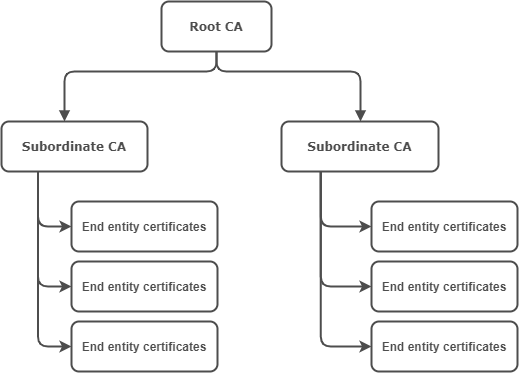
\includegraphics[scale=0.4]{images/CA} 
\caption{Vereinfachte Darstellung des Certificate Authority Aufbaus.}
\label{fig:CA}
\end{center}
\end{figure}	

\indent OpenWrt zeigt zusätzlich einige Schwächen bei der Implementierung von Sicherheitsmaßnahmen gegen Bruteforce Angriffe (vgl. Abschnitt \ref{bruteforce}) auf den Login-Bereich (vgl. Abbildung \ref{fig:bf_regression}) sowie gegen Session-Hijacking Attacken. Da OpenWrt durchaus die fehlgeschlagenen Login-Versuche registriert, wäre ein Zähler die einfachste Option Bruteforce Angriffe auf die Login-Bereiche zu verhindern. Es könnten z.B. eine begrenzte Anzahl an Versuchen zur Verfügung stehen. Nachdem diese abgelaufen sind, muss eine gewisse Zeit gewartet werden, bis ein neuer Versuch unternommen werden kann. Ebenso könnte ein \mbox Zeitlimit zwischen jedem Login-Versuch implementiert werden, sodass ein Angriff verlangsamt wird. Wenn das Passwort ausreichend komplex gewählt ist, so würde dies die Geschwindigkeit und Attraktivität von Bruteforce Angriffen deutlich mindern. Session-Hijacking Angriffe könnten verhindert werden, wenn zusätzlich zu den "`anti-cross-site-forgery-request“ (anti-CSFR)–Token (vgl. Abschnitt \ref{CSRF}) der "`Session-Timer“ verringert würde. Das kontinuierliche, automatische Updaten der auf der Seite dargestellten Informationen setzt diesen Timer jedoch alle fünf Sekunden zurück. Dieses Verhalten muss unterbunden werden. 300 Sekunden (5 Minuten) für eine Sitzung wären ein geeigneteres Intervall anstelle von den derzeit eingesetzt 3600 Sekunden (60 \mbox Minuten). 


\begin{figure}[ht]
\centering
\subfloat[Teilbild 1: Antwortzeiten des Webservers]{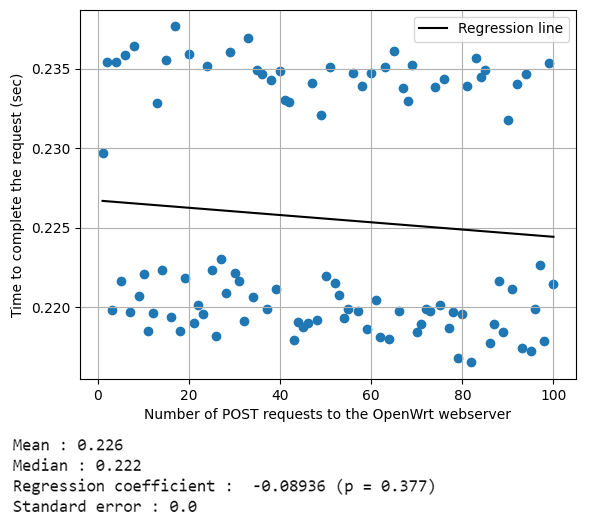
\includegraphics[width=0.48\hsize]{images/TP_D_11_2_login_attempts_luci}}
\hspace*{0.05\hsize}
\subfloat[Teilbild 2: Antwortzeiten des SSH-Servers]{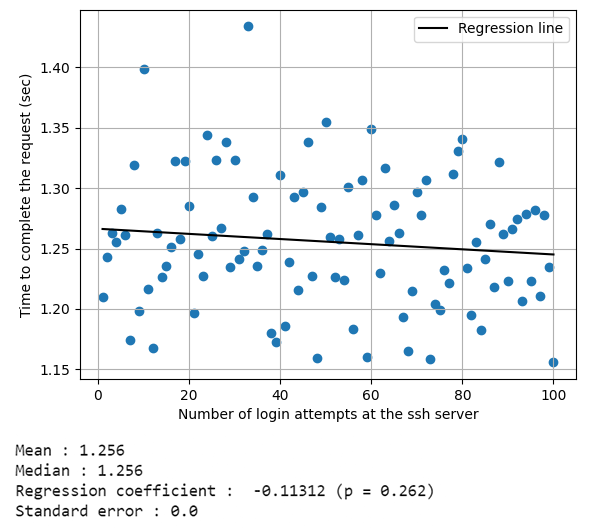
\includegraphics[width=0.48\hsize]{images/TP_D_11_2_ssh_login_attempts}}
\caption{Antwortzeiten des Web-Servers und des SSH-Servers bei wiederholten Login-Versuchen. Die Regressionslinie zeigt, dass die Antwortzeiten konstant bleiben bzw. sogar tendenziell geringer werden. Ebenso sind der Durchschnitt, der Median, der Regressionskoeffizient und der Standardfehler dargestellt.}
\label{fig:bf_regression}
\end{figure}


\indent	
Abschließend deckte die Durchführung der Technischen Richtlinie noch einen weiteren Schwachpunkt des OpenWrt Betriebssystems auf. Die Testfälle TR.E.5 bis TR.E.8 wurden alle nicht bestanden, da es keinen automatischen Authentifizierungsmechanismus gibt, welcher Firmware-Updates prüft. Dem Nutzer werden lediglich signierte SHA256 Hash-Werte des Firmware-Updates zur Verfügung gestellt, sodass die Authentizität und Integrität der Datei vom Nutzer geprüft werden muss. 
\begin{quote}
"` […] while release image files are usually signed by one or more developers with detached GPG signatures to allow users to verify the integrity of installation files.
[…]
Note that not every file is signed individually but that we’re signing the sha256sums or - for repositories - the Packages files to establish a chain of trust: The SHA256 checksum will verify the integrity of the actual file while the signature will verify the integrity of the file containing the checksums. \cite{OpenWrtWebseite.2020b}“
\end{quote}
\vfill \pagebreak

\noindent Dieser Ansatz bietet natürlich nur die geforderten Schutzziele, wenn ein Nutzer tatsächlich die Authentizität und Integrität der sha256sums Datei prüft und anschließend den darin enthalten Hash-Wert mit dem der heruntergeladenen Datei vergleicht. Ebenso wie der OPKG Paket Manager könnte auch der Firmware-Update-Mechanismus auf die usign Ed22519 \mbox Signaturen zurückgreifen oder eine GPG-Signatur der Entwickler tragen. Eine automatische Verifizierung der Signatur über das Internet, mit entsprechenden Sicherheitsmaßnahmen, wäre dann möglich. In den Fällen, in denen das Gerät keine Internetverbindung aufweist, könnte dann auf die SHA256 Hash-Werte zurückgefallen werden. Durch das beschriebene Vorgehen könnte das Gerät TR.E.5 bis TR.E.8 bestehen sowie den Nutzern mehr Sicherheit und Nutzerfreundlichkeit bieten. 	\\ \indent
	In einigen Fällen lässt sich keine sinnvolle Lösung finden, die für ein Projekt wie OpenWrt geeignet ist. So auch bei TR.D.24, welches fordert, dass dem Nutzer eine Nachricht auf dem Gerät angezeigt wird, wenn eine neue Firmware verfügbar ist. Für diese Anforderung müsste das Gerät mit dem Internet verbunden sein und zudem müssten von Seiten der OpenWrt Entwickler ein Update-Server zur Verfügung gestellt werden. Dies würde Kosten auf Seiten der freiwilligen Entwickler sowie eine größere Angriffsoberfläche auf Seiten der Nutzer verursachen. Eine Anmeldung beim E-Mail Newsletter der Entwickler wäre die simpelste Möglichkeit um über neue Versionen sowie Sicherheitslücken informiert zu bleiben. 

\end{onehalfspace}



\section[Ergebnisse und Gegenüberstellung]{Ergebnisse der statischen Code-Analyse sowie Gegenüberstellung mit ausgewählten Ergebnissen des Home Router Security Reports 2020}
\label{erg_statisch}
\begin{onehalfspace}
Im Rahmen dieser statischen Code-Analyse durch das \glqq Firmware Analysis and Comparison Tool \grqq{} des FKIE wurden sieben verschiedene quelloffene Router-Firmware Alternativen analysiert. Dabei waren fünf Fragen von besonderem Interesse. 

\begin{itemize}
\item Wann wurde das letzte Update für das Gerät veröffentlicht?
\item Welches Betriebssystem wird verwendet und wie viele kritische Schwachstellen sind für dieses bekannt?
\item Welche vorbeugenden Maßnahmen gegen Exploits werden eingesetzt und wie häufig sind diese aktiviert.
\item Ist privates kryptografisches Schlüsselmaterial enthalten?
\item Können hartkodierte Login-Daten und bekannte Passwörter in dem Firmware-Abbild gefunden werden?
\end{itemize}

\noindent FACT konnte während der Analyse erfolgreich 92,73\% der Daten aus den Firmware-Abbildern extrahieren. Bei der gesamten betrachteten Firmware wurde durch Analyse von Metadaten eine MIPS 32-Bit Architektur mit "`big-endian“ Byte-Reihenfolge festgestellt. Dies hat zwar keinen direkten Einfluss auf die Sicherheit eines Gerätes, jedoch ist diese Architektur nicht quelloffen und die Entwicklung ist in den letzten Jahren ins Stocken geraten \cite{Halfacree.2020}. Für die Analyse der "`Critial Vulnerabilities and Exposures“ (CVE) (vgl. Abschnitt \ref{CVE}) wurde aufgrund einiger Fehler in FACT nicht das Ergebnis der automatischen Analyse gewählt. Stattdessen wurden die Ergebnisse durch die Webseite www.cvedetails.com, welche wiederum auf die Daten der "`National Vulnerability Database\grqq{} der US-Regierung, zugreift, bereitgestellt. Da cvedetail.com ausschließlich CVSS v2 Bewertungen (siehe Abschnitt \ref{CVE}) bereitstellt, wurden einzig diese für die Analyse verwendet. Um Vergleichbarkeit mit den Ergebnissen des FKIE zu gewährleisten wurden lediglich CVE-Einträge mit einem Schweregrad von "`Hoch“ (vgl. Tabelle \ref{tab:CVSS dif}) gezählt.

\end{onehalfspace}

\subsection{Vergangene Tage seit der letzten Veröffentlichung eines Firmware-Updates}
\begin{onehalfspace}
In diesem Abschnitt soll evaluiert werden, wann für die betrachteten Firmware-Abbilder das letzte Mal eine neue Version seit dem 24.12.2020 veröffentlicht wurde. Alle Abbilder des Firmware-Corpus spezifizierten das Veröffentlichungsdatum im Dateinamen selbst oder auf der jeweiligen Webseite. Dieses Kriterium wurde untersucht, da es die Bereitschaft der Entwickler andeutet, ihr Projekt regelmäßig mit Funktions- und Sicherheitsupdates zu unterstützen. Eine neuere Version bedeutet also zumeist, dass weniger sicherheitsrelevante Lücken bekannt sind und das System sicherer ist. Da die Unterstützer der quelloffenen Projekte in vielen Instanzen auf weitere Software zurückgreifen und auch diese Updates erfährt, ist es wahrscheinlich, dass Firmware bekannte Lücken hat, wenn diese längere Zeit nicht erneuert wurde. \\ \indent
 	Grafik \ref{fig:Days since Update} zeigt, dass für fünf von sieben untersuchten Firmware-Abbildern in den letzten 365 Tagen eine neue Version veröffentlicht wurde. Aufgrund des Ausreißers in den erhobenen Daten wird im Folgenden der Median statt des Mittelwertes betrachtet.  Es ergibt sich, dass die Router-Betriebssysteme nach Median-Berechnung alle 83 Tage und im Schnitt alle 309 Tage eine neue Version erhalten. Ebenfalls muss erwähnt werden, dass bei der Veröffentlichung einer neuen Version meist alle von dem jeweiligen Projekt unterstützen Geräte diese neue Version zur Verfügung gestellt bekommen. So werden bei einer neuen Version von OpenWrt alle ca. 1700 Geräte von diesem neuen Update unterstützt und erfahren somit alle Sicherheitsupdates, die bereitgestellt werden. Dies steht im Gegensatz zu etablierten Herstellern von Routern, welche oft pro Gerät eine eigene Version entwickeln. Gargoyle Router Management wurden nicht in den letzten 365 Tagen erneuert und das Tomato Betriebssystem hat in den letzten 1480 Tagen kein Update erfahren. Der Zyklus von 83 Tagen ist höher als der Update-Zyklus von Desktop- oder Server-Betriebssystemen, jedoch noch im Rahmen der 90 Tage, welche normalerweise das Zeitfenster darstellen, in dem Entwickler Zeit haben auf Sicherheitslücken und Probleme zu reagieren (\glqq responsible disclosure\grqq ) \cite{Lazarov.2019}. Darüber hinaus muss besonders darauf hingewiesen werden, dass in manchen Fällen ein Paketmanager (vgl. Abschnitt \ref{OpenWrt}) zur Verfügung steht, über welchen Updates für Pakete während der Laufzeit installiert werden können. Somit sind Updates der Firmware nur notwendig, um Kernfunktionalität zu erweitern oder Fehler in dieser zu beheben, sowie um den Kernel zu aktualisieren. Nur eine von acht bisher veröffentlichten Sicherheitslücken im Jahr 2020 konnte ausschließlich durch ein Update auf eine neuere Version von OpenWrt behoben werden, wobei alle weiteren durch ein einfaches Update des betroffenen Paketes nachgebessert werden konnten \cite{OpenWrtSecurity}. In proprietärer Firmware ist ein Paketmanager für die Installation von zusätzlicher Software und für das Herunterladen von Updates in den meisten Fällen nicht vorhanden. Verglichen mit den Ergebnissen des \glqq Home Router Security Reports 2020\grqq{} zeigt sich, dass für die quelloffenen Betriebssysteme häufiger neue Versionen veröffentlicht werden. Wenn man die analysierten Abbilder als Gruppe betrachtet, dann schneidet diese vergleichsweise gut ab. Einzig Tomato fällt als Ausreißer heraus. Lediglich ASUS, AVM und Netgear, als Hersteller von handelsüblichen Routern, können mithalten.	 \\ \indent
 	Ebenso wie im \glqq Home Router Security Report 2020\grqq{} festgestellt, muss zusätzlich beachtet werden, dass alle betrachteten Produkte kleinere Updates auch über die Geräte selbst zu Verfügung stellen könnten, sodass die aktuellste Version nicht im Internet veröffentlicht wird. Darüber hinaus handelt es sich bei den hier festgestellten Daten ausschließlich um eine Momentaufnahme, die keine Aussagekraft darüber hat, ob regelmäßig Updates bereitgestellt werden, oder ob diese Sicherheitslücken überhaupt adressieren \cite{PeterWeidenbachJohannesvomDorp.2020}.


\begin{figure}[ht]
\begin{center}
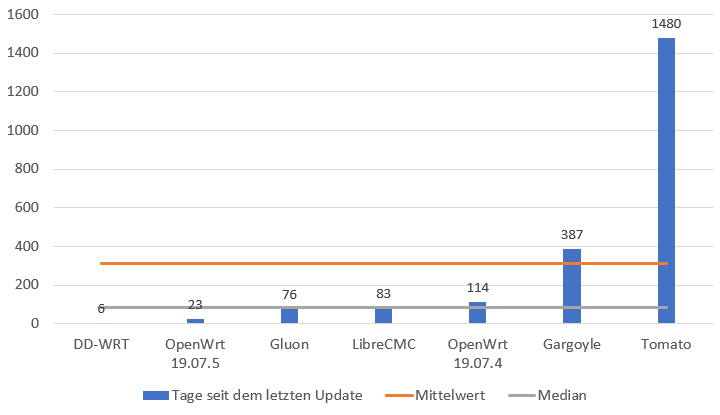
\includegraphics[scale=0.5]{images/days_since_update} 
\caption{Vergangene Tage seit der letzten Aktualisierung der betrachteten Firmware. Seit dem letzten Update von DD-WRT ist am geringsten Zeit vergangen. Für Tomato ist seit 1480 Tagen keine neue Version erschienen. (Stand: 30.12.2020)}
\label{fig:Days since Update}
\end{center}
\end{figure}	


\end{onehalfspace}



\subsection{Betriebssysteme}
\begin{onehalfspace}
Da es sich bei allen analysierten Firmware-Abbildern um quelloffene Projekte handelt, ist es nicht verwunderlich, dass der Linux-Kernel dominant vertreten ist. Der Linux-Kernel, welcher 1991 von Linus Tovalds entwickelt wurde und seither stetig weiterentwickelt wird stellt einen der am häufigsten genutzten Betriebssysteme für IoT Geräte dar \cite{Gaur.13.05.201515.05.2015}. Die geringe Größe des Kernels, der große Funktionsumfang und die umfangreiche Dokumentation und Verbreitung sind für eine community-getriebene Entwicklung auf speicher- und rechenleistungslimitierten Geräten wie z. B. Heim-Routern gut geeignet.  Grafik \ref{fig:Linux Kernel} zeigt, dass alle untersuchten Projekte einen Linux Kernel verwenden. Dieser Trend deckt sich ebenfalls mit den Ergebnissen des \glqq Home Router Security Reports\grqq{} des FKIE. In den untersuchten Produkten des Verbrauchermarktes wurde Linux in 91\% der Fälle verwendet \cite[p.~2]{PeterWeidenbachJohannesvomDorp.2020}.\\ 

\begin{figure}[ht]
\begin{center}
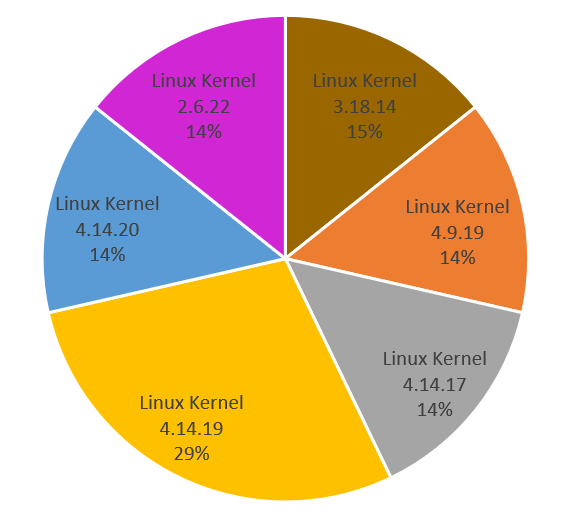
\includegraphics[scale=0.45]{images/linux_kernel} 
\caption{Verwendete Linux Kernel der betrachteten Firmware.}
\label{fig:Linux Kernel}
\end{center}
\end{figure}

Aufgrund der unzureichenden Ergebnisse der FACT-Analyse bezüglich der vorhandenen CVE-Einträge für die verwendeten Linux-Kernel wurden die Ergebnisse in diesem Fall direkt über \glqq www.cvedetails.com\grqq{} abgerufen. FACT erstellt zunächst eine "`Common Platform Enumeration“ (CPE) der Software Version und stellt mit dieser CPE eine Anfrage an die "`National Vulnerability Database“. Da die zurückgegebenen Ergebnisse allerdings auch Schwachstellen beinhalten, welche nur für bestimme Geräte mit der jeweiligen Linux-Kernel Version gelten, wurden die jeweiligen Schwachstellen des Kernels über die \mbox Website \glqq cvedetail.com\grqq{} abgefragt. Bei einer Stichprobe der von FACT gelieferten CVE-Einträge sind verschiedene Einträge aufgefallen, welche z.B. nur für bestimmte IoT-Geräte wie Smartwatches eingetragen sind. Cvedetail nutzt ebenfalls die "`National Vulnerability Database“, stellt jedoch noch zusätzliche Informationen und  Statistiken bereit. Auf diese Art wurde \mbox sichergestellt, dass die betrachteten Schwachstellen spezifisch für den Kernel sind und nicht für ein bestimmtes Gerät, welches diesen Kernel nutzt. Da nicht alle eingetragenen CVEs eine direkte Bedrohung darstellen, wurden die Ergebnisse weiter eingeschränkt. So wurden lediglich solche CVEs betrachtet, welche mit einen CVSS2 Wert von sieben oder höher eingestuft wurden. Wie Grafik \ref{fig:Firmware CVE Numbers} zeigt, stehen für alle betrachteten Geräte einige CVE Einträge des Linux Kernels zur Verfügung. Ebenfalls kann man sehen, dass der in DD-WRT verwendete Kernel mehr CVE-Einträge hat als der von Gargoyle Router Management, obwohl bei DD-WRT die geringste Zeit seitdem letzten Firmware Update vergangen ist. Tomato schneidet erneut am schlechtesten ab. Grafik \ref{fig:Linux Kernel Timeline} zeigt zusätzlich, dass für zwei der sechs verschiedenen Linux Kernel schon seit einigen Jahren keine Sicherheitsupdates entwickelt werden. Sowohl der von Tomato verwendete Kernel, 2.6.22, als auch Linux Kernel 3.8.14, welcher von DD-WRT verwendet wird, werden nicht mehr mit Updates unterstützt. Dies spiegelt sich auch in der hohen Anzahl CVE-Einträge wider (siehe Abbildung \ref{fig:Firmware CVE Numbers}).

\begin{figure}[ht]
\begin{center}
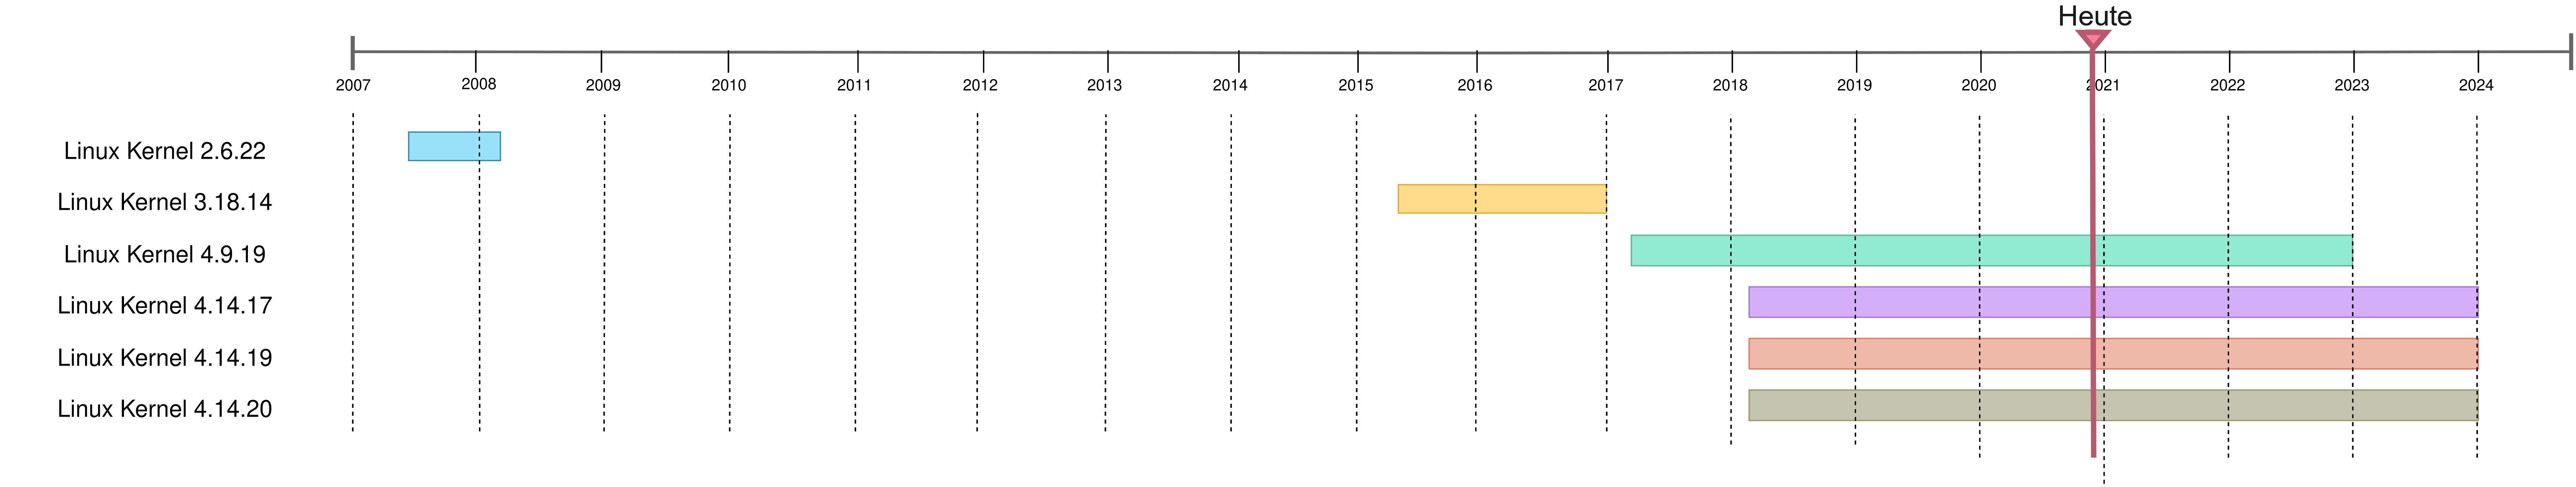
\includegraphics[scale=0.3]{images/Timeline-Linux-Kernel} 
\caption{Stellt jeweils den Zeitraum von Veröffentlichung bis zum Ende der Entwicklerunterstützung für alle gefundenen Linux Kernel dar. Der Kernel 4.14.19 wurde in zwei Firmware-Abbildern genutzt.}
\label{fig:Linux Kernel Timeline}
\end{center}
\end{figure}


\begin{figure}[ht]
\begin{center}
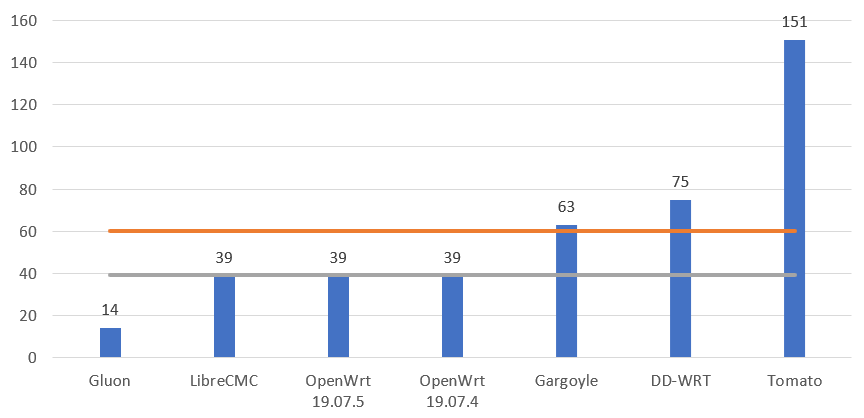
\includegraphics[scale=0.5]{images/number_of_cves} 
\caption{Anzahl der gefundenen CVE-Einträge pro Firmware mit einer CVSS-Einschätzung von sieben oder höher.}
\label{fig:Firmware CVE Numbers}
\end{center}
\end{figure}

Die Ergebnisse sind aufgrund der unterschiedlichen Beschaffung sowie der fehlenden CVSS3 Werte nicht wirklich mit denen des \glqq Home Router Security Reports 2020\grqq{} vergleichbar. Jedoch kann man sagen, dass die quelloffenen Router-Betriebssysteme mehrheitlich modernere Linux-Kernel Versionen nutzen. Lediglich zwei der betrachteten Firmware-Abbilder nutzen einen Kernel, der nicht mehr unterstützt wird. Der \glqq Security Report\grqq{} gibt an, dass ein Drittel der betrachteten Geräte einen Kernel vor Version 3 nutzen und lediglich ca. 22\% einen aktuellen Kernel der 4. Version \cite[p.~8]{PeterWeidenbachJohannesvomDorp.2020}. Im Gegensatz dazu nutzen ca. 70\% der betrachteten quelloffenen Software-Projekte einen Linux-Kernel der Version 4.9.19 oder höher (siehe Abbildung \ref{fig:Linux Kernel Timeline}). \\ \indent
Im Gegensatz zu den Ergebnissen des \glqq Security Reports\grqq{} können falsch positive Ergebnisse bei der Erkennung der Kernel Version beinahe ausgeschlossen werden, da diese ebenfalls von den Entwicklern auf der Webseite oder in den Veröffentlichungsdokumenten der jeweiligen Version veröffentlicht wird. Jedoch besteht die Möglichkeit, dass die Entwickler eigene Korrekturen für Sicherheitslücken des Kernels entwickeln und veröffentlichen. Dies ist bei dieser Art community-getriebener Entwicklung nicht unwahrscheinlich, da hier keine Entwickler bezahlt werden müssen, welche zusätzlich zu ihren anderen Aufgaben für das Beheben von Sicherheitslücken im Kernel eingesetzt werden. Ebenfalls ist es möglich, dass aufgrund der uneindeutigen CPE-Spezifikation einige CVE-Einträge nicht von \mbox \glqq cvedetails.com\grqq{} gelistet werden \cite[p.~7]{PeterWeidenbachJohannesvomDorp.2020}.	

\end{onehalfspace}


\subsection{Härtungsmaßnahmen}
\begin{onehalfspace}
FACT ist in der Lage die folgenden Exploit Mitigationsmaßnahmen (siehe Abschnitt \ref{Hardening}) zu identifizieren:

\begin{itemize}
\setlength\itemsep{0.01em}
\item Stack Canary
\item FORTIFY\_SOURCE
\item NX
\item PIE
\item RELRO
\end{itemize}


\noindent Sowohl RELRO als auch das NX-Bit werden vermehrt bei den quelloffenen Router-Betriebssystemen eingesetzt (siehe Abbildung \ref{fig:Firmware Hardening Net}). Außer Tomato nutzen alle der betrachteten Firmwares zu beinahe 100\% das NX-Bit. Mit Ausnahme von Tomato und DD-WRT nutzen im Schnitt ca. 50\% aller ausführbarer Dateien der Firmware-Abbilder RELRO. Tomato und DD-WRT setzen hingegen kaum auf RELRO. PIE wird andererseits im Schnitt zu ca. 40\% genutzt. Tomato scheint bevorzugt auf PIE zu setzen (siehe Abbildung \ref{fig:Firmware Hardening Bar}). Die Nutzung von Stack Canaries und FORTIFY\_SOURCE verhält sich pro Firmware nahezu identisch. Gargoyle Router Management, LibreCMC und OpenWrt nutzen es bei ca. 19\% aller Dateien, Gluon bei ca. 8\%, während DD-WRT und Tomato beinahe vollständig auf diese Techniken verzichten. 
Die Verbreitung von PIE ist vergleichbar mit den Ergebnissen der FKIE Veröffentlichung (siehe Abbildung \ref{fig:Firmware Hardening Net}) \cite[p.~15]{PeterWeidenbachJohannesvomDorp.2020}. Ebenso wie im \glqq Security Report\grqq{} berichtet, nutzen auch die quelloffenen Betriebssysteme annähernd alle vollumfänglich NX-Bits. Dies lässt sich leicht durch den vergleichsweise guten Schutz bei infinitesimalen Geschwindigkeitseinbußen erklären. Die Daten des FKIE zeigten, dass RELRO nur selten von allen Herstellern eingesetzt wird mit Ausnahme von AVM. Dem steht eine Nutzung von ca. 50\% bei den freien Firmware-Produkten gegenüber. Ebenso wie die betrachtete Firmware der Markthersteller, wird nur selten auf Stack Canaries und FORTIFY\_SOURCE gesetzt. Obwohl Stack Canaries keinen merkbaren Einfluss auf die Geschwindigkeit eines Systems hat, scheint diese Technik nur bei wenigen Dateien angewendet worden zu sein. Es könnte sich hierbei um systemkritische Dateien handeln. Dies gilt ebenso für die FORTIFY\_SOURCE Option (siehe Abbildung \ref{fig:Firmware Hardening Bar}). \\ 


\begin{figure}[ht]
\begin{center}
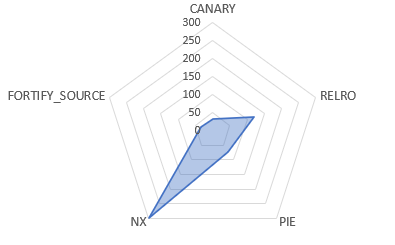
\includegraphics[scale=0.65]{images/hardening_open_source} 
\caption{Netzdiagramm (Kiviat-Diagramm, Radardiagramm) der verwendeten Härtungsmaßnahmen. Es werden alle Firmware-Abbilder gemeinsam dargestellt. NX, RELRO und PIE werden am häufigsten genutzt. Stack Canaries und FORTIFY\_SOURCE wird kaum eingesetzt.}
\label{fig:Firmware Hardening Net}
\end{center}
\end{figure}


\begin{figure}[ht]
\begin{center}
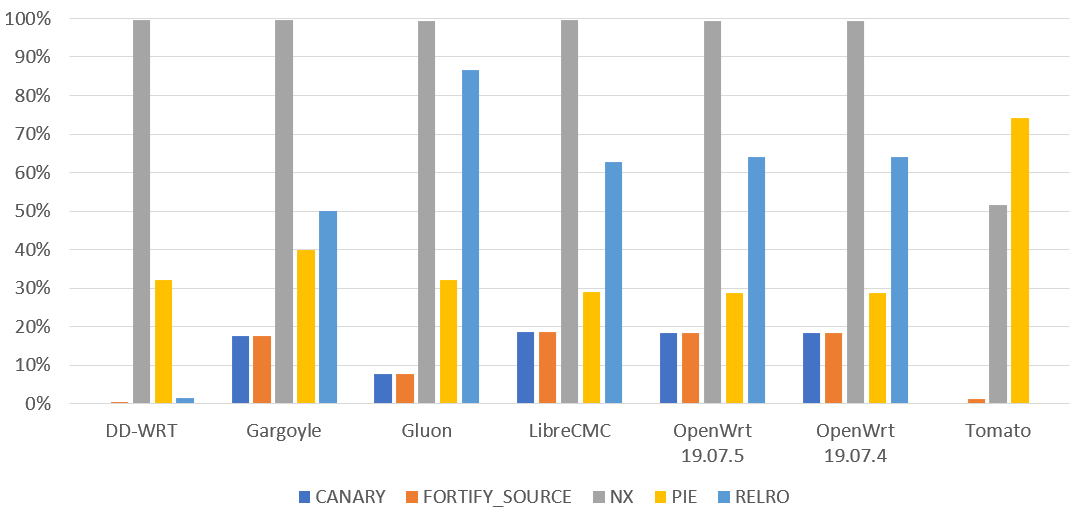
\includegraphics[scale=0.5]{images/hardening_open_source_all} 
\caption{Säulendiagramm der verwendeten Härtungsmaßnahmen nach Analyse der FACT Daten. Pro Firmware sind Stack Canaries, FORTIFY\_SOURCE, NX, PIE und RELRO dargestellt.}
\label{fig:Firmware Hardening Bar}
\end{center}
\end{figure}



\indent Zusammenfassend kann man sagen, dass vor allem auf NX und RELRO für den Großteil der Dateien gesetzt wird. PIE, Stack Canaries und FORTIFY\_SOURCE wird nur bei wenigen ausführbaren Dateien genutzt. 

\end{onehalfspace}


\subsection{Privates Schlüsselmaterial}
\begin{onehalfspace}
Wenn private kryptographische Schlüssel in den Firmware-Abbildern enthalten sind, so haben diese keine Sicherheitsfunktion mehr. Um die korrekte Funktionalität zu gewährleisten, in dem Fall, dass private Schlüssel enthalten sein müssen, so sollten die Vorgaben der OWASP eingehalten werden:
\end{onehalfspace}

\begin{quote}
“Do not hardcode secrets such as passwords, usernames, tokens, private keys or similar variants into firmware release images. This also includes the storage of sensitive data that is written to disk. If hardware security element (SE) or Trusted Execution Environment (TEE) is available, it is recommended to utilize such features for storing sensitive data. Otherwise, use of strong cryptography should be evaluated to protect the data. If possible, all sensitive data in clear-text should be ephemeral by nature and reside in a volatile memory only \cite{OWASPEmbeddedApplicationSecurityProject.2019}.”
\end{quote}

\begin{onehalfspace}
\noindent
 Die Einhaltung dieser Vorgaben ist jedoch deutlich erschwert, wenn die Firmware nicht spezifisch für ein Gerät geschrieben ist. Ebenso stehen den Entwicklern der quelloffenen Firmware nicht alle Entwicklerwerkzeuge der Hersteller zur Verfügung um z.B. auf ein "`Hardware Security Element“ zuzugreifen. Zugleich wird für den Zugriff in einigen Fällen ein physischer Zugang zu dem Gerät benötigt. 	\\ \indent
	Trotz dieser Probleme konnte FACT nur aus DD-WRT und Gargoyle Router \mbox Management private Schlüssel extrahieren. Bei beiden Betriebssystemen wurden jeweils ein Pkcs8PrivateKey sowie ein SSLPrivateKey gefunden. Da PKCS\#8 ein Container-Format für private kryptographische Schlüssel ist, kann man ohne weitere Nachforschung nicht bestimmen, welchen Nutzen diese Schlüssel für die Systeme haben. Die gefundenen SSL-Schlüssel dienen vermutlich dazu den vom Webbrowser an den Webserver gesendeten Session-Key zu entschlüsseln \cite{sslKeys.}. Es lässt sich also vermuten, dass DD-WRT und Gargoyle Transport Layer Security verwenden, jedoch kann ein Man-in-the-Middle Angriff einfach durchgeführt werden, wenn der private SSL Schlüssel bekannt ist \cite{Du.21.10.201123.10.2011}. Die genauen Details der Implementierung und Nutzung der gefundenen Schlüssel ist jedoch vollkommen unbekannt. Es könnte sich ebenso um ungenutztes oder veraltetes Material handeln. Darüber hinaus könnte der SSL Schlüssel auch nur für die initiale Konfiguration des Gerätes genutzt werden, um danach durch einen neuen ersetzt zu werden. 
	

\begin{figure}[ht]
\centering
\subfloat[Teilbild 1: Quelloffene Betriebssysteme]{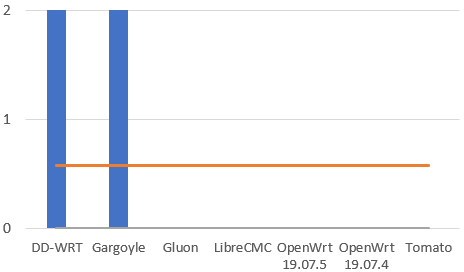
\includegraphics[width=0.45\hsize]{images/number_of_priv_keys}}
\hspace*{0.05\hsize}
\subfloat[Teilbild 2: Ergebnisse der FKIE Untersuchung]{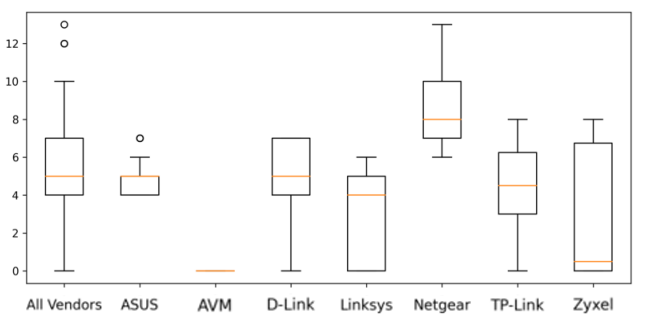
\includegraphics[width=0.5\hsize]{images/number_of_priv_keys_FKIE}}
\caption{\\Teilbild 1: Anzahl der privaten Schlüssel in den untersuchten quelloffenen Betriebssystemen. Lediglich in DD-WRT und Gargoyle wurden private Schlüssel gefunden. \\ Teilbild 2: Anzahl der privaten Schlüssel in der vom FKIE untersuchten Firmware. Außer bei AVM wurden bei allen Hersteller private Schlüssel gefunden \cite[p.~17]{PeterWeidenbachJohannesvomDorp.2020}.}
\label{fig:Firmware Private Keys}
\end{figure}


\end{onehalfspace}


\subsection{Angelegte Benutzeraccounts}
\begin{onehalfspace}
Diese Analyse dient dazu hartkodierte Accountinformationen in der untersuchten Firmware zu finden. FACT extrahiert dazu die Daten aus der "`/etc/shadow“ und "`/etc/passwd“ Datei. Diesen Dateien speichern Informationen zu allen Nutzeraccounts, welche auf dem System angelegt sind. Dazu gehören unter anderem der Nutzername, das Passwort, die Nutzerrechte und weitere Informationen der Nutzer. Das Passwort, welches in der "`/etc/shadow“ Datei gespeichert wird, liegt in Hash-Form vor. FACT nutzt eine Passwortliste mit häufig genutzten Passwörtern und das Programm \glqq john\grqq{}, um das Passwort im Klartext darzustellen. Problematisch sind bereits angelegte Nutzeraccounts vor allem, wenn diese nicht geändert oder abgeschaltet werden können. Ebenso bergen sie das Risiko, dass ein unerfahrener Nutzer diesen Account benutzt, ohne ein neues Password für den Account festzulegen. Auf diese Art kann ein Angreifer sehr einfach auf die Konfiguration des Gerätes zugreifen. \\ \indent	
	Die Analyse der quelloffenen Firmware zeigt, dass lediglich Gargoyle Router Management einen bereits angelegten Nutzeraccount mit schwachem Passwort ausweist. Im Test des FKIE wurden auf 50 Geräten (40\%) vom Hersteller angelegte Accounts gefunden \cite[p.~19]{PeterWeidenbachJohannesvomDorp.2020}. Da es sich bei dem Befund des Gargoyle Betriebssystems allerdings um den root Account handelt, ist es nicht unwahrscheinlich, dass der Nutzer nach einmaliger Eingabe des Passwortes "`password“ ein neues Passwort wählen muss. In diesem Falle bietet Gargoyle Router Management nicht mehr Sicherheit als OpenWrt, bei welchem der root Account ohne Passwort initialisiert ist. In dieser Instanz ist es umso wichtiger, dass der Nutzer auf das Risiko ausreichend hingewiesen wird, bzw. aufgefordert wird, dass Passwort zu ändern.
\end{onehalfspace}



\chapter{Diskussion}
\label{discussion}
\section{Limitationen}
\label{limits}
\begin{onehalfspace}
Eine mögliche Limitation bei der Durchführung der Technischen Richtlinie ist die Testumgebung. Besonders die double NAT Konfiguration (vgl. Abschnitt \ref{umgebung})  ist nicht optimal zur Durchführung der Technischen Richtlinie. Der beschriebene Aufbau kann dazu führen, dass einige Ergebnisse nicht zuverlässig angegeben werden können, vor allem wenn der Zugriff auf die Konfiguration des ersten Routers oder des Modems nicht gegeben ist. So könnten einige Pakete nicht zum eigentlichen OpenWrt Router zugstellt werden, wenn diese bereits von der vorgelagerten Firewall abgefangen wurden. Ebenfalls hätte ein zusätzlicher Testrechner und ggf. weitere Router den Testvorgang weiter beschleunigt, indem nmap-Scans über Nacht oder parallel ausgeführt hätten werden können. Ebenso hätte dies die Durchführung einiger zusätzlicher Tests erlaubt, welche nun als "`inconclusive“ markiert wurden, da nicht genug Systeme zur Verfügung standen, um die vorgegebene Testprozedur durchzuführen. Des Weiteren musste in diesem Falle das \glqq Conformance Statement\grqq{} der Technischen Richtlinie vom Tester selbst ausgefüllt werden, statt vom Hersteller oder Entwickler. Dies stellt eine sehr einseitige Betrachtung des Gerätes durch den Tester dar. Auch könnte hier eine gewisse Voreingenommenheit unterstellt werden, da der Tester ggf. gewisse Ergebnisse bereits erwartet. Anschließend muss an dieser Stelle ebenso betrachtet werden, dass die Möglichkeit besteht, bereits bei der Anfertigung des \glqq Conformance Statements\grqq{} etwas zu übersehen, wodurch Ergebnisse der TR verfälscht werden können. \\ \indent
 	Eine weitere Limitation zeigt sich im Zusammenspiel von OpenWrt und der Technischen Richtlinie selbst. OpenWrt ist zwar durchaus für Heim-Router und Router aus dem SOHO-Bereich gedacht, jedoch müssen die Nutzer schon für die Installation einige technische Grundkenntnisse vorweisen, sowie überhaupt von der Möglichkeit wissen. So wird OpenWrt durch die TR an einigen Stellen für die Umsetzung von Funktionen bestraft, welche für den durchschnittlichen Nutzer von OpenWrt vielleicht geeignet sind. Darüber hinaus darf die TR nur als ein Mittel von vielen gesehen werden, um die Sicherheit solcher komplexen Systeme zu untersuchen. Es ist vielmehr das Ziel der Technischen Richtlinie ein Grundmaß an Sicherheit auf Heim-Routern zu schaffen, statt in jeder Hinsicht sichere Router. Aus diesem Grunde geht die Richtlinie zu Teilen tiefer in Details hinein als anderswo, wo die Existenz einer Funktion wichtiger ist als die perfekte Implementierung. Auch wirkt die Technische Richtlinie nicht direkt automatisierten Angriffen wie Heartbleed, Sambacry  oder BCMUPnP entgegen \cite{Carvalho.2014, Carvalho.2014, Konoth.29.01.2019}. Die TR sorgt allerdings für eine verringerte Angriffsoberfläche und viele Maßnahmen, die den Nutzer dabei unterstützen sollen, sein Gerät sicherer zu betreiben. Schon sicherere Login- und WLAN-Passwörter können einige Angriffe verlangsamen und uninteressant machen. Die Technische Richtlinie sollte also lediglich als Teil des Weges zu sichereren Geräten verstanden werden. Weitere Techniken zum Testen von Software sollten dennoch weiter eingesetzt werden, um einen weiteren Blick auf die IT-Sicherheitslage zu bekommen. 	\\ \indent
	Zu den genannten Limitationen kommt zusätzlich eine zeitliche Komponente. Die Durchführung anhand von OpenWrt war im gesetzten zeitlichen Rahmen machbar, jedoch wäre es dennoch interessant gewesen, eine möglichst vollständige Durchführung der TR anzustreben. OpenWrt hätten durch den Paket-Manager sämtliche zusätzlichen Komponenten geboten, um jedes Modul der TR vollständig zu testen. Dies hätte als konzeptioneller Beweis weitere Einblicke in die Möglichkeiten und Limitationen der Technischen Richtlinie und auch OpenWrt gegeben. Ebenso interessant wie die Ergebnisse von OpenWrt bei der TR wäre ein Vergleich mit dem Resultat von anderen handelsüblichen Routern. Der Zertifizierungsprozess hat jedoch erst vor kurzem begonnen und die Daten der bisher durchgeführten Testdurchläufe stehen nicht für die Öffentlichkeit zur Verfügung. So wird es noch eine Weile dauern, bis Vergleichswerte verfügbar sind.	\\ \indent
	Neben den Limitationen bezüglich der Technischen Richtlinie, müssen auch einige Einschränkungen bei der Durchführung der statischen Code-Analyse aufgezeigt werden. Die betrachteten Firmware Abbilder hätten schneller und ausführlicher analysiert werden können, wenn mehr Zeit und mehr Rechenkapazitäten zur Verfügung gestanden hätten. Neben den gewählten Metriken liefert FACT noch weitere interessante Plug-ins. Ebenso kann nur eine eingeschränkte Vergleichbarkeit mit den Ergebnissen des \glqq Home Router Security Reports 2020\grqq{} dargestellt werden. Dies liegt unter Anderem an der geringen Anzahl an untersuchter Firmware. Im Gegensatz zu den Herstellern, welche im FKIE Report betrachtet wurden, wird bei der quelloffenen Firmware in den meisten Fällen eine Codebasis für alle unterstützen Geräte kompiliert, sodass es die Ergebnisse nicht beeinflusst hätte, wenn Firmware für verschiedene Prozessorinstruktionssätze vertreten gewesen wäre. Ebenfalls wurden in dieser Analyse bereits die bekanntesten quelloffenen Alternativen betrachtet, welche gefunden werden konnten. Ein weiterer Punkt, welcher die Vergleichbarkeit mit dem \glqq Home Router Security Report 2020\grqq{} betrifft, war die Analyse der veröffentlichten CVE-Einträge pro verwendetem Linux-Kernel. So lassen sich diese Werte zwar nicht direkt vergleichen, jedoch geben die Angaben des FKIE Reports und der in dieser Arbeit aufgeführten Analyse einen Einblick in die Lage der IT-Sicherheit der betrachteten Geräte.
\end{onehalfspace}


\section{Implikationen und zukünftige Forschung}
\label{implikationen}
\begin{onehalfspace}
Die Ergebnisse zeigen, dass die Technischen Richtlinie durchaus auch für quelloffenen Router-Betriebssysteme geeignet ist. Nur aufgrund der relativ guten Ergebnisse von \mbox OpenWrt kann man jedoch nicht sagen, dass es sich hier von einem IT-Sicherheitsstandpunkt aus um ein sicheres System handelt. Lediglich ein Mindestmaß an Sicherheit kann festgestellt werden und für das vollständige Bestehen der TR sind noch einige Änderungen notwendig. Ebenso wurden nur einige Tests mit FACT durchgeführt, sodass auch in dieser Hinsicht nicht von einem vollständig nachgewiesen sicheren System gesprochen werden darf. Es handelt sich hier nur um Indikatoren und Momentaufnahmen. FACT selbst erweist sich jedoch als geeignetes Programm, um mit wenig Aufwand und geringen technischen Fähigkeiten eine statische Code-Analyse an Firmware durchzuführen.  \\ \indent
	Zukünftig wäre ein Vergleich verschiedener Geräte anhand der Technischen Richtlinie von Interesse. Ebenso wäre die Durchführung an anderen quelloffenen Router-Betriebssystemen sowie eine Gegenüberstellung interessant. Wie bereits erwähnt wäre es zusätzlich eine Möglichkeit die TR vollständig anhand von OpenWrt durchzuführen und darüber hinaus mithilfe des \glqq Software Developer Kits\grqq{} (SDK) der OpenWrt-Entwickler eine Version bereitzustellen, welche alle Anforderungen der TR erfüllt. Weiterhin kann eine sinnvolle Erweiterung der Technischen Richtlinie um mehr Testfälle in Betracht gezogen werden. Auf diese Weise könnte mehr Funktionalität geprüft werden oder bereits geprüfte Funktionen eingehender getestet werden. Wenn die Verbreitung der TR fortgeschritten ist und mehrere Geräte eine Zertifizierung erhalten haben, so wäre eine Marktanalyse interessant. So könnte die Auswirkung der TR auf die Hersteller und auf die Wahrnehmung der Kunden betrachtet werden.
\end{onehalfspace}

\vfill \pagebreak 

%###############################################################################

%\chapter{Fazit}


%###############################################################################
% Literaturverzeichnis und ggfs. Index

\cleardoublepage
\addcontentsline{toc}{chapter}{Literaturverzeichnis}
\bibliography{literatur}

% soweit gewünscht: Tabellen- und Abbildungsverzeichnis
\cleardoublepage
%\listoftables              % Tabellenverzeichnis
%\listoffigures             % Abbildungsverzeichnis



%###############################################################################
% Danksagung




%###############################################################################
% Appendix (falls nötig)

\cleardoublepage
\addcontentsline{toc}{chapter}{Anhang}
\begin{appendix}           % Anhang

\chapter{Verwendete Firmware für FACT Analyse}

\begin{table}[ht]
\centering
\resizebox{\textwidth}{!}{%
\begin{tabular}{lllll}
\textbf{PROJEKT} &
  \textbf{ROUTER} &
  \textbf{VERSION} &
  \textbf{\begin{tabular}[c]{@{}l@{}}VERÖFFENTLICHUNGS-\\ DATUM\end{tabular}} &
  \textbf{LINK} \\ \hline
OPENWRT &
  ARCHER C7 v5 &
  19.07.4 &
  09.2020 &
  \begin{tabular}[c]{@{}l@{}}https://downloads.openwrt.org/releases/19.07.4/\\ targets/ath79/generic/openwrt-19.07.4-ath79-\\ generic-tplink\_archer-a7-v5-squashfs-factory.bin\end{tabular} \\
OPENWRT &
  ARCHER C7 v5 &
  19.07.5 &
  12.2020 &
  \begin{tabular}[c]{@{}l@{}}https://downloads.openwrt.org/releases/19.07.5/\\ targets/ath79/generic/openwrt-19.07.5-ath79-\\ generic-tplink\_archer-c7-v5-squashfs-factory.bin\end{tabular} \\
LIBRECMC &
  ARCHER C7 v2 &
  v1.5.3:2020-10-02 &
  02.10.2020 &
  \begin{tabular}[c]{@{}l@{}}https://librecmc.org/librecmc/downloads/\\ snapshots/v1.5.3/targets/ath79/generic/librecmc\\ -ath79-generic-tplink\_archer-c7-v2-squashfs-factory.bin\end{tabular} \\
GLUON &
  ARCHER C7 v5 &
  V2-v2020.2.1 &
  09.10.2020 &
  \begin{tabular}[c]{@{}l@{}}https://images.ffkbu.de/BonnV2/stable/Wireguard/factory/\\ gluon-ffkbu-V2-v2020.2.1-Wireguard-tp-link-archer-c7-v5.bin\end{tabular} \\
GARGOYLE &
  ARCHER C7 v5 &
  1.12.0 (stable) &
  03.12.2019 &
  \begin{tabular}[c]{@{}l@{}}https://www.gargoyle-router.com/downloads/images/ar71xx/\\ gargoyle\_1.12.0-ar71xx-generic-archer-c7-v5-squashfs-factory.bin\end{tabular} \\
TOMATO &
  NETGEAR WNDR3700v3 &
  3.4-138 &
  05.12.2016 &
  https://advancedtomato.com/downloads/router/wndr3700v3 \\
DDWRT &
  ARCHER C7 v5 &
  12-18-2020-r45036 &
  18.12.2020 &
  \begin{tabular}[c]{@{}l@{}}ftp://ftp.dd-wrt.com/betas/2020/12-18-2020-r45036/\\ tplink\_archer-c7-v5/\end{tabular}
\end{tabular}%
}
\end{table}



\chapter{OpenWrt Veröffentlichungshistorie}
\begin{table}[ht]
\centering
\def\arraystretch{1}
\begin{tabular}{llll}
\hline
\textbf{Version (Code Name)} & \textbf{Veröffentlichungsdatum} & \textbf{Linux Kernel} & \textbf{libc} \\ \hline
White Russian 0.9 & 2007 January & 2.4.30 & \multirow{13}{*}{uClibc} \\ \cline{1-3}
Kamikaze 7.06 & 2007 June & 2.6.19 &  \\ \cline{1-3}
Kamikaze 7.07 & 2007 July & \multirow{2}{*}{2.6.21} &  \\ \cline{1-2}
Kamikaze 7.09 & 2007 September &  &  \\ \cline{1-3}
Kamikaze 8.09 & 2008 September & 2.6.26 &  \\ \cline{1-3}
Kamikaze 8.09.1 & 2009 June & \multirow{2}{*}{2.6.26.8} &  \\ \cline{1-2}
Kamikaze 8.09.2 & 2010 January &  &  \\ \cline{1-3}
Backfire 10.03 & 2010 April & \multirow{2}{*}{2.6.32} &  \\ \cline{1-2}
Backfire 10.03.1 & 2011 December &  &  \\ \cline{1-3}
Attitude Adjustment 12.09 & 2013 April & 3.3 &  \\ \cline{1-3}
Barrier Breaker 14.07 & 2014 October & 3.10.49 &  \\ \cline{1-3}
Chaos Calmer 15.05 & 2015 September & 3.18.20 &  \\ \cline{1-3}
Chaos Calmer 15.05.1 & 2016 March & 3.18.23 &  \\ \hline
LEDE 17.01.0 & 2017 February & 4.4.50 & \multirow{21}{*}{musl} \\ \cline{1-3}
LEDE 17.01.1 & 2017 April & 4.4.61 &  \\ \cline{1-3}
LEDE 17.01.2 & 2017 June & 4.4.71 &  \\ \cline{1-3}
LEDE 17.01.3 & 2017 August & 4.4.89 &  \\ \cline{1-3}
LEDE 17.01.4 & 2017 October & 4.4.92 &  \\ \cline{1-3}
LEDE 17.01.5 & 2018 July & 4.4.140 &  \\ \cline{1-3}
LEDE 17.01.6 & 2018 September & 4.4.153 &  \\ \cline{1-3}
OpenWrt 18.06.0 & 2018 July & 4.9.111, 4.14.52 &  \\ \cline{1-3}
OpenWrt 18.06.1 & 2018 August & 4.9.120, 4.14.63 &  \\ \cline{1-3}
OpenWrt 18.06.2 & 2019 February & 4.9.152, 4.14.95 &  \\ \cline{1-3}
OpenWrt 18.06.3 & skipped & skipped &  \\ \cline{1-3}
OpenWrt 18.06.4 & 2019 July & 4.9.184, 4.14.131 &  \\ \cline{1-3}
OpenWrt 18.06.5 & 2019 November & 4.9.198, 4.14.151 &  \\ \cline{1-3}
OpenWrt 18.06.6 & 2020 January & 4.9.208, 4.14.162 &  \\ \cline{1-3}
OpenWrt 18.06.7 & 2020 January & 4.9.211, 4.14.167 &  \\ \cline{1-3}
OpenWrt 18.06.8 & 2020 March & 4.9.214, 4.14.171 &  \\ \cline{1-3}
OpenWrt 19.07.0 & 2020 January & 4.14.162 &  \\ \cline{1-3}
OpenWrt 19.07.1 & 2020 January & 4.14.167 &  \\ \cline{1-3}
OpenWrt 19.07.2 & 2020 March & 4.14.171 &  \\ \cline{1-3}
OpenWrt 19.07.3 & 2020 May & 4.14.180 &  \\ \cline{1-3}
OpenWrt 19.07.4 & 2020 September & 4.14.195 &  \\ \cline{1-3}
OpenWrt 19.07.5 & 2020 December & 4.14.209 & \\ \hline
\end{tabular}
\caption{Veröffentlichungshistorie von OpenWrt, sowie genutzer Linux Kernel und libc Version}
\label{tab:OpenWrt_History}
\end{table}

\end{appendix}

\end{large}
%###############################################################################

\end{document}

%###############################################################################
